%                                     
%                                                                             
%  MMO    MM   MMMMMM  MMMMMMM   MM    MMMMMMMM   MMD   MM  MMMMMMM MMMMMMM   
%  MMM   MMM   MM        MM     ?MMM              MMM$  MM  MM         MM     
%  MMMM 7MMM   MM        MM     MM8M    MMMMMMM   MMMMD MM  MM         MM     
%  MM MMMMMM   MMMMMM    MM    MM  MM             MM MMDMM  MMMMMM     MM     
%  MM  MM MM   MM        MM    MMMMMM             MM  MMMM  MM         MM     
%  MM     MM   MMMMMM    MM   MM    MM            MM   MMM  MMMMMMM    MM
%
%
%            - META-NET Language Whitepaper | Bulgarian paper -
% 
% ----------------------------------------------------------------------------

\documentclass[]{../../metanetpaper}

%!TEX TS-program = xelatex
\RequireXeTeX %Force XeTeX check

\usepackage{polyglossia}
\setotherlanguages{bulgarian,english}

\usepackage{ulem}\normalem

\title{Българският език в дигиталната епоха --- The Bulgarian
  Language\ \ \ \ in the\ \ \ \ \ Digital Age}

\subtitle{White Paper Series --- Серия „Бели книги“}

\author{
 Diana Blagoeva~  {\small Bulgarian Academy of Sciences}\\
 Svetla Koeva~ {\small Bulgarian Academy of Sciences}\\
 Vladko~Murdarov~  {\small Bulgarian~Academy~of~Sciences}
}
\editors{
  Georg Rehm, Hans Uszkoreit\\(FIXME, \textcolor{grey1}{editors})
}

\begin{document}

\maketitle

\null
\pagestyle{empty} 

\FundingLNotice{\selectlanguage{bulgarian} Авторите на този документ
  благодарят сърдечно на авторите на Бялата книга за немски за
  предоставената възможност да използват избрани езиково независими
  части.
  
  \bigskip
  Разработката на настоящата Бяла книга е финансирана по Седма рамкова
  програма и Програма ICT Policy Support Programme на Европейската
  комисия, договори T4ME (договор за финансиране 249119), CESAR
  (договор за финансиране 271022), METANET4U (договор за финансиране
  270893) и META-NORD (договор за финансиране 270899).}

\FundingRNotice{\selectlanguage{english} The authors of this document
  are grateful to the authors of the White Paper on German for
  permission to re-use selected language-independent materials from
  their document.
  
  \bigskip
  The development of this white paper has been funded by the Seventh
  Framework Programme and the ICT Policy Support Programme of the
  European Commission under the contracts T4ME (Grant Agreement
  249119), CESAR (Grant Agreement 271022), METANET4U (Grant Agreement
  270893) and META-NORD (Grant Agreement 270899).}

\makefundingnotice

\pagenumbering{Roman} 
\setcounter{page}{5}
\pagestyle{scrheadings}

\cleardoublepage

% --------------------------------------------------------------------------
\bsection*{Предговор --- Preface}

\begin{Parallel}[c]{78mm}{78mm}
\ParallelLText{\selectlanguage{bulgarian}
Бялата книга е част от
 серия документи, представящи развитието в областта на
 езиковите технологии и техния потенциал. Документите са предназначени за
преподаватели, журналисти, политици, различни езикови
 общности и т. н.
 
Достъпът до езикови технологии за езиците, които
 се говорят в Европа, е много различен. Затова и необходимите действия за подкрепа на изследванията и развитието
 на езиковите технологии също са различни. Те зависят от много фактори, например сложността на даден език и броя на
неговите носители.

META-NET, мрежа за високи постижения, изградена с
подкрепата на Европейската комисия, извършва анализ на съществуващите езикови ресурси и технологии.
 Анализът е съсредоточен върху 23-те официални европейски езика, наред с други по-важни национални и регионални езици. Резултатите показват значителни липси за всеки език.
 Задълбоченият експертен анализ и оценка на актуалната
 ситуация ще помогнат за увеличаване на ефекта от
изследванията и намаляване на риска от
 пропуски.

В META-NET участват 54 изследователски центъра от 33
 страни, работещи съвместно с търговски и правителствени организации, научни институции, софтуерни
 компании, фирми за информационни технологии и
 европейски университети. Заедно те разработват
 технологична визия и стратегическа научна програма, която показва как езиковите технологии могат да отговорят на научните предизвикателства до 2020 г.}

\ParallelRText{\selectlanguage{english}
This white paper is part of a series that promotes knowledge about language technology and its potential. It addresses journalists, politicians, language communities, educators and others. 
The availability and use of language technology in Europe varies between languages. Consequently, the actions that are required to further support research and development of language technologies also differ. The required actions depend on many factors, such as the complexity of a given language and the size of its community.

META-NET, a Network of Excellence funded by the European Commission, has conducted an  analysis of current language resources and technologies in this white paper series (p.~\pageref{whitepaperseries}). The analysis focused on the 23 official European languages as well as other important national and regional languages in Europe. The results of this analysis suggest that there are tremendous deficits in technology support and significant research gaps for each language. The given detailed expert analysis and assessment of the current situation will help maximise the impact of additional research.

As of November 2011, META-NET consists of 54 research centres from 33 European countries (p.~\pageref{metanetmembers}). META-NET is working with stakeholders from economy (software companies, technology providers and users), government agencies, research organisations, non-governmental organisations, language communities and European universities. Together with these communities, META-NET is creating a common technology vision and strategic research agenda for multilingual Europe 2020.} 
\ParallelPar
\end{Parallel}

\cleardoublepage

% --------------------------------------------------------------------------
\bsection*{Съдържание --- Table of Contents}

\tableofcontents

\addtocontents{toc}{\protect\thispagestyle{empty}\protect}
\addtocontents{toc}{{\Large\textsf{\centerline{ЕЗИЦИТЕ В ЕВРОПЕЙСКОТО ЕЗИКОВО ИНФОРМАЦИОННО ОБЩЕСТВО}}\par}}

\cleardoublepage

% --------------------------------------------------------------------------
\setcounter{page}{1}
\pagenumbering{arabic} 
\pagestyle{scrheadings}


% Start of original language part
% --------------------------------------------------------------------------
\ssection[Резюме]{Резюме}

\selectlanguage{german}

\begin{multicols}{2}
Много европейски езици могат да изчезнат в дигиталната епоха, защото не са представени в интернет и не разполагат с достатъчно електронни ресурси. Възможности за търговия с голям потенциал за развитие остават неизползвани поради езиковите бариери. Ако не бъдат предприети незабавни действия, много граждани на Европа ще се окажат в неравностойно социално и икономическо положение, тъй като говорят само родния си език. 
 
Езиковите технологии ще дадат възможност на европейските граждани да живеят равнопоставено в икономически развито  общество, основано на знания и информация. Езиковите технологии са пътят към бърза, евтина и леснодостъпна комуникация, прехвърляща езиковите граници. 

Услугите, базирани на езикови технологии,  в по-голямата си част са платени и се предлагат от американски компании. Безплатната услуга Google Translate е единичен случай. Успехът на Watson, компютърна система на IBM, която победи хора в играта  Jeopardy, свидетелства за огромния потенциал на езиковите технологии. Като европейци трябва да си зададем няколко много важни въпроса:

\begin{itemize}
\item Трябва ли нашата комуникация и научна инфраструктура да зависят от монополистични компании?
\item Можем ли да си позволим да разчитаме на услуги, свързани с обработката на езика, които във всеки момент могат да бъдат прекратени? 
\item Има ли партньори от други континенти, които биха участвали при решаването на проблемите с превода и други въпроси, свързани с европейското многоезичие?
\item Ще помогне ли европейско културно наследство за оформянето на общество, основано на знания,  предлагайки по-добри, по-сигурни, по-прецизни, по-новаторски и устойчиви висококачествени технологии?
\end{itemize}

Бялата книга за български доказва, че в България съществува общност, занимаваща се с изследване и развитие на езиковите технологии. Трябва да се отбележи обаче, че в областта на езиковите технологии в момента работят предимно малки и средни предприятия, които не са конкурентноспособни на световния пазар.

Въпреки че за български език са разработени някои езикови ресурси и технологии, те са значително по-малко на брой и с по-ниско качество в сравнение с тези за английски.

На основа на оценката, представена в този документ, става ясно, че трябва да бъдат предприети незабавни действия, за да се осигури напредък в развитието на езиковите технологии за български език.
\end{multicols}

\clearpage

% --------------------------------------------------------------------------
\ssection[Заплаха за езиците и предизвикателство пред езиковите технологии]{Заплаха за езиците и предизвикателство пред езиковите технологии}

\begin{multicols}{2}

Свидетели сме на дигитална революция, която съществено промени комуникациите и обществото. Съвременното развитие на информационните и  комуникационните технологии понякога се сравнява с въвеждането на печатарската преса от Гутенберг. Как тази аналогия ни позволява да погледнем в бъдещето на европейското информационно общество и нашите езици?

След откритието на Гутенберг истински преломи в комуникацията и обмена на знания са постижения от ранга на превода на библията на говорим език от Мартин Лутер. В следващите
 столетия се наблюдава сериозно развитие, за да се достигне до
обработка на естествения език и бърз обмен на информация:

\begin{itemize}
\item стандартизацията на правописа и граматиката осигурява по-бързо разпространение на нови идеи и научни открития;
\item появата на книжовните езици позволява на гражданите да общуват в рамките на определени  (често политически) общности;
\item езиковото обучение и преводът улесняват обмена на информация;
\item  създаването на редакторски и библиографски стандарти осигурява качество и лесен достъп до публикуваните материали;
\item появата на различни медии - вестници, радио, телевизия, книги и други - отговаря на нуждата от различни типове комуникация.
\end{itemize}

В последните 20 години с помощта на информационните технологии много от тези процеси се автоматизират и улесняват:

\begin{itemize}
\item Софтуерът за електронно публикуване замества пишещите и печатарските машини.
\item Microsoft PowerPoint (и други) заменя прожекционните апарати.
\item Документите се изпращат и получават по-бързо по имейл, отколкото по факс.
\item Skype (и други) позволява евтини телефонни разговори по интернет и виртуални срещи.
\item Форматите за аудио и видео улесняват обмена на мултимедийно съдържание.
\item Търсачките осигуряват достъп до уеб страници по ключови думи.
\item Онлайн услугите като \selectlanguage{english} Google Translate \selectlanguage{bulgarian} осигуряват бърз приблизителен превод.
\item Социалните медии като  \selectlanguage{english} Facebook,  Twitter  и  Google+ \selectlanguage{bulgarian}  улесняват общуването, сътрудничеството и обмена на информация.
\end{itemize}

Макар подобни приложения да са полезни, те не могат да предложат достатъчно ефективна подкрепа за устойчиво развитие на многоезиковото европейско общество, в което информация и стоки се придвижват свободно.

\subsection{Езиковите граници като пречка пред европейското информационно общество}
  
Не можем да предвидим с точност как ще изглежда
бъдещото информационно общество. Много вероятно е обаче революцията в комуникационните технологии да свързва по непознати досега начини хората, говорещи различни езици.
Възниква необходимостта да се учат нови езици и да се създават нови езикови приложения, за да се осигури взаимното разбиране и достъп до съдържание. В глобалното икономическо и информационно пространство обменът на информация на множество езици е по-бърз с помощта на новите медии. Високата популярност на социалните мрежи \selectlanguage{english} (Wikipedia, Facebook, Twitter, YouTube, Google+) \selectlanguage{bulgarian} е само върхът на айсберга.

Днес прехвърляме гигабайтове текст от една точка на света до друга за няколко секунди, преди да разберем, че е написан на език, който не познаваме. Според скорошно проучване, изготвено по поръчка на Европейската
 комисия, 57\% от потребителите на интернет в Европа
 купуват стоки и услуги на езици, които не са им родни
 (най-разпространен е английският, следван от
 френски, немски и испански). 55\% от потребителите на интернет четат съдържание на чужди езици, докато само 35\% използват чужд език, когато пишат имейли или публикуват съобщения и коментари онлайн \cite{EC1}. Преди няколко
 години английският е бил lingua franca в интернет. Сега обаче ситуацията е коренно променена след  рязкото нарастване  на броя на публикациите на други езици (разпространени например в Азия и Средния изток). Дигиталното разединение, произтичащо от езиковите бариери, 
 изненадващо не привлича достатъчно внимание в публичното
 пространство. И все пак именно то поставя неотложния
 въпрос: Кои европейски езици ще се развият в съвременното информационно общество, основано на знания, и кои са осъдени да изчезнат?

\subsection{Рискът за нашите езици}

Печатарската преса засилва обмена на информация в Европа, но същевременно води до отмирането на много европейски езици. Текстове на регионални и малцинствени езици се публикуват рядко, а  езици като корнуолски и далматински са ограничени до говоримата си форма. Възможно ли е интернет да има същото влияние?

Близо  80-те езика, които се говорят в Европа, са сред
 най-богатото и важно културно наследство на Стария континент и съществен  компонент от уникалния му социален модел  \cite{EC2}. Популярни езици като английски или испански ще продължат да съществуват в условията на развиващия се дигитален пазар, но много европейски езици може да се окажат
с ограничена употреба в интернет. Това би намалило глобалните позиции на Европа и е в противоречие със стратегическите цели за равно участие на всеки европейски
 гражданин, независимо от езика, на който говори. Според доклад на ЮНЕСКО за многоезичието  езиците са важен посредник за осигуряване на
фундаментални  човешки права, като правото
 на изразяване на политически убеждения, правото на образование и участие в обществото \cite{Unesco1}.

\subsection{Езиковите технологии предоставят възможности}

В миналото усилията за запазване на езиците са били насочени
 към езиковото обучение и превода. Според някои
 изчисления през 2008 г. европейският пазар за писмен и
 устен превод, локализация на софтуер и превод на
 уеб сайтове се е равнявал на 8,4 милиарда евро и се
 очаква да нараства с 10\% на година \cite{EC3}. Тези данни отразяват малък процент от днешните и бъдещите нужди при комуникацията на различни езици.
Пълноценното използване на европейските езици в бъдеще може да се осигури от подходящи езикови технологии, аналогично на технологиите за осигуряване  на енергия, транспорт и равен достъп за хората с увреждания.  

Езиковите технологии (насочени към всички видове писмен и говорим текст) помагат на хората да си сътрудничат, да работят заедно, да споделят знание и да участват в социалния и
 политическия живот независимо от езиковите бариери и компютърните си умения. Тези технологии са вградени в сложни компютърни системи, за да ни помогнат да:

\begin{itemize}
\item търсим информация в интернет;
\item проверяваме правописа и граматиката в текстообработваща програма;
\item разглеждаме предложенията в онлайн магазин;
\item слушаме гласови инструкции на навигационна система;
\item превеждаме уеб страници онлайн.
\end{itemize}

Езиковите технологии се използват в някои основни приложения, които участват в широка мрежа от продукти. Предназначението на Белите книги на META-NET е да се анализира дали основните езикови приложения са налице за всеки европейски език.

За да запази предните си позиции в световните иновации, Европа се нуждае от стабилни и финансово достъпни езикови технологии, приложими за всички европейски езици и интегрирани в ключови софтуерни системи.
В близко бъдеще работата на потребителя в интерактивна, мултимедийна и многоезикова  среда ще е  невъзможна
без посредничеството на езиковите технологии.

\subsection{Възможности за езиковите технологии}

В света на печатното слово технологичната революция започва с бързото възпроизвеждане на текстове с помощта на печатарска преса, задвижвана от механична сила. Трудната работа по проверката, редакцията, превода и обобщаването на съдържание обаче се е извършвала от хора. Откритието на Едисън позволява да се правят записи – но тази технология просто създава аналогови копия.

Днес езиковите технологии могат да автоматизират процесите на превод, създаване на съдържание и управление на информация и знания на всички европейски езици. Тези технологии могат да помогнат за развитието на интуитивни
 езиково базирани приложения за домашна електротехника, съоръжения, автомобили, компютри и роботи. Въпреки че прототипите
 за някои от тях все още са в начален стадий, подемът на изследванията и разработките през последните години разкрива множество реални възможности. Машинният превод например вече е достигнал сравнителна точност в някои специализирани области, а
 експерименталните приложения осигуряват възможности за управление на
 многоезикова информация и знание, както и за
 създаване на съдържание на много европейски езици.

Както при повечето технологии първите езикови приложения - гласов
 интерфейс и диалогови системи - са предназначени за тясно специализирани области и често са с ограничени възможности. 
 Съществуват значителни пазарни ниши в образователната и развлекателната индустрия за интегриране на  езикови технологии в образователно-развлекателни  игри и програми, сайтове, посветени на културното наследство, софтуер за библиотеки и издателства, симулационни и тренировъчни системи. 
Мобилните услуги, приложенията за компютърно подпомогнато езиково или електронно обучение, както и софтуерът за разпознаване
 на плагиатство и за самооценка, са само някои от областите, в които езиковите технологии могат да имат съществено приложение. Нарастващата популярност на социалните мрежи като Twitter и Facebook предполага използването на езиковите технологии за мониторинг, обобщение на дискусии, анализ на мнения, разпознаване на емоции, както и за идентифициране на нарушени авторски права.

Езиковите технологии предлагат огромни възможности за Европейския
 съюз. Те могат да помогнат при решаването на проблеми, свързани с многоезичието в Европа – при едновременното използване на различни езици във фирми, организации и образователни институции. Жителите на Европа трябва  да общуват без езикови граници, все още валидни за единния европейски пазар.  Езиковите технологии могат да преодолеят тази бариера, подкрепяйки едновременно с това равнопоставеността при използването на езиците. 
В по-далечното бъдеще европейските (много)езикови технологии могат да дадат пример за подпомагане на развитието на многоезикови общества по света.
 Езиковите технологии могат да се възприемат като „помощни“ технологии, които помагат за преодоляване на проблемите на лингвистичното многообразие и за подобряване на комуникацията между общности, говорещи различни езици.

Област на активни изследвания е използването на езиковите технологии при спасителни операции в райони, засегнати от природни бедствия, където
 точността на информацията може да е въпрос на живот и смърт. Бъдещите интелигентни роботи с възможности за комуникация на много езици ще имат потенциал да спасяват човешки живот.

\subsection{Предизвикателства пред езиковите технологии}

Макар че езиковите технологии отбелязаха значителен
 напредък през последните години,
 технологичният прогрес и създаването на иновациионни продукти значително изостават. Широко използваните технологии като програми за проверка на правопис и граматика, интегрирани в съвременните текстообработващи системи, 
обикновено са едноезикови и достъпни само за ограничен брой езици. 
Онлайн услугите за машинен превод, макар че са полезни за бързо генериране на приблизителен превод, са напълно неподходящи за точен и цялостен превод. Поради комплексността на човешките езици моделирането им в компютърни програми и тестването на моделите в реалния свят е продължителна и скъпа дейност, която изисква трайни финансови ангажименти.  
Европа трябва да поддържа водещата си роля при посрещане на технологичните предизвикателства на многоезиковото общество посредством нови ефективни методи за развитие. Това включва както напредък в информационните технологии, така и използване на съвременни техники при програмирането.

\subsection{Как хората и машините учат език?}

За да разберем как компютрите обработват езиковата информация и защо се затрудняват с тази задача, нека хвърлим поглед към начина, по който хората научават родния си език и чужди езици. След това
 накратко ще бъде представен начинът, по който работят системите, базирани на езикови технологии.

Човек усвоява езика по два различни механизма. Детето
 научава родния си език, като възприема общуването между
 носители на езика – родители, братя, сестри и други
 членове на семейството. От около двегодишна възраст децата започват да формулират първите си думи и кратки фрази. Това е възможно, тъй като хората имат генетичната способност да имитират и комбинират.

Усвояването на втори език на по-късна възраст обикновено изисква
 повече усилия, тъй като детето не живее сред
 носителите на езика. В училище чуждите езици най-често се изучават с помощта на абстрактни правила, парадигми и примерни текстове, илюстриращи  граматическата структура, речника и правописа на даден език. С възрастта  усвояването на чужд език става все по-трудно.

Двата основни типа системи, базирани на езикови технологии, „усвояват“ езика по подобен начин. Статистическите („базирани на данни“) подходи извличат
 лингвистични знания от големи корпуси от текстове. Докато  за тренирането на приложения за проверка на правописа са достатъчни текстове само на един език, то за тренирането на система за машинен превод са нужни паралелни текстове на два (или повече) езика. Алгоритмите за извличане на информация всъщност „научават“ моделите, по които думи, кратки
 фрази или цели изречения се превеждат от един на друг език. 

Статистическите методи понякога изискват милиони изречения, като качеството на резултатите се увеличава заедно с големината на анализирания
 текст. Това е една от причините, поради които компаниите, разработващи системи за търсене, се стремят да съберат колкото
 може повече езикови данни. Програмите за проверка на
 правописа и услуги като Googlе Search и Google Translate разчитат на статистически подходи. Основното предимство на статистиката е, че моделите се извличат много бързо чрез последователни тренировъчни цикли, макар че качеството на тези методи може да варира в значителна степен.

Вторият подход към езиковите технологии и особено към машинния превод се основава на лингвистични правила. Експерти - лингвисти, компютърни лингвисти и програмисти, формулират  граматически правила (правила за превод) и съставят
 речникови списъци (лексикони). Изграждането на системи, основани на правила, изисква много време и човешки труд. 
Някои от водещите системи за машинен превод, базирани на правила, се
 изграждат в продължение на повече от 20 години. Основното предимство
 на тези системи е, че експертите могат в по-голяма степен да контролират обработката на езиковата информация. 
Това осигурява възможността за бърза корекция на грешки в софтуера и
съобразяване с изискванията на потребителите, особено в случаите, когато системите, базирани на лингвистични правила, се използват в езиковото обучение.
Поради финансови ограничения подобни приложения се разработват само за
 по-разпространените езици.

Тъй като силните и слабите страни на статистическите системи и системите, базирани на лингвистични правила, обикновено се допълват взаимно, в момента изследванията са ориентирани към хибридни подходи, които комбинират  двата метода. Засега хибридните подходи се прилагат с по-слаб успех в практическите разработки в сравнение с научните изследвания. 

Както личи от тази глава, много от приложенията, които се използват в момента от информационното общество, разчитат в значителна степен на езиковите технологии. По отношение на многоезичието това важи с особена сила за европейското икономическо и информационно пространство. Макар че през последните години езиковите технологии отбелязват значителен напредък, все още има сериозен потенциал за повишаване на  качеството на техните приложения. Следващата част ще хвърли светлина върху мястото на българския език в европейското информаци
 онно общество и върху състоянието на езиковите технологии за български.  
\end{multicols}

\clearpage

% --------------------------------------------------------------------------
\ssection[Българският език в европейското информационно общество]{Българският език в европейското информационно общество}

\begin{multicols}{2}

\subsection{Общи данни}
Българският език е официалният език в Република България.

Говори се от близо 9 милиона души предимно в
 България, но също и в Гърция, Македония, Румъния,
 Сърбия, Турция (европейската
 част), Украйна, Австралия, Канада, САЩ, Германия и Испания. По-големи общности от говорещи български
 са регистрирани и в Хърватия, Чешката република,
 Унгария, Израел, Либия, Молдова, Руската федерация
 (европейската част), Словакия \cite{Ethno}. Агенцията за българите
 в чужбина \cite{ABA} към Министерския съвет отговаря за
 българските общности в съседните на България страни и имигрантските общности в различни държави по света.

Предварителните данни на Националния статистически
 институт \cite{NSI} след преброяването на населението на
 България показват, че към 1 февруари 2011 г.
 населението на страната е 7 351 633 души. Колко
 българи живеят в страни от Европейския съюз ще стане
 ясно през 2012 г., когато ще бъдат публикувани данните
 от преброяването и в тези държави.

Официалната азбука за писане на български език е кирилицата. Българският е първият славянски език, който разполага със собствена писмена система, датираща от 9-ти век на н. е. През 886 г. България приема глаголическата азбука, създадена от св.
 св. Кирил и Методий, която постепенно е заменена от кирилицата
 – азбука, създадена и наложена от Охридската и
 Преславската книжовна школа в началото на 10-ти век. На 1
 януари 2007 г., когато България е приета за пълноправен
 член на Европейския съюз, кирилицата става третата
 официална азбука на Европейския съюз след латинската
 и гръцката.

Българските диалекти са регионалните говорими варианти на българския език, разпространени
 както в границите на страната, така и извън тях. Българските диалекти са разделени на западни и
 източни от т. нар. „ятова граница“, която разграничава
 две по-големи диалектни области въз основа на
 различните звукови варианти на старобългарската
 гласна „ят“ (
\includegraphics[scale=0.32]{../_media/bulgarian/yat}), произнасяна в определени условия като
 ['a] или [e] на изток от границата (например в ед. ч.
 [{\it б'ал}], но в мн. ч. [{\it бели}]) или само като [e] на запад от
 ятовата граница (ед. ч. [{\it бел}] и мн. ч. [{\it бели}]).

\subsection{Особености на българския език}

Българският език принадлежи към групата на южнославянските езици и едновременно с това е част от
 т. нар. Балкански езиков съюз (Balkan Sprachbund), поради което има характеристики и на двете езикови групи. Като славянски език българският притежава богата флективна и деривационна система, а глаголите са
 разделени по двойки въз основа на техния аспект. Поради взаимното влияние между езиците в Балканския езиков съюз българският губи падежите при
 имената (с изключение на звателната форма) и
 инфинитива при глагола.

Освен общата лексика, някои от най-важните граматически характеристики на българския език, които го отличават като славянски език (част от тях споделени и с други балкански езици), са:

\begin{itemize}
\item Богата флективна система. Богатата флективна
система до известна степен затруднява работата в областта на
 езиковите технологии.
 При лематизация например могат да възникнат
 проблеми при разпознаване
 на
 частите на речта. Думата \textit{бели} например е омограф и
 може да означава: 

\begin{itemize}
\item форма за мн. ч. на съществителното \textit{беля};
\item форма за мн. ч. на прилагателното \textit{бял};
\item форма за 3 лице, ед. ч., сегашно време на глагола
 \textit{беля};
\item форма за 2 или 3 лице, ед. ч., минало свършено време
 на глагола \textit{беля};
\item форма за 2 лице, ед. ч., повелително наклонение на
 глагола \textit{беля}.
\end{itemize}

\item Богата деривационна система: умалителни и увеличителни съществителни: {\it стол – столче}; суфикси
 за женски род на съществителните за лица (професии): {\it учител – учителка}; и други.
\item Видови двойки при глаголите: {\it родя – раждам};
\item Свободно изпускане на подлога (име или местоимение), защото глаголното окончание носи информация за вършителя на действието: \textit{Аз чета книга. — Чета книга.}
\end{itemize}

В хода на историческото развитие на българския език и
 контактите му със съседните неславянски езици на Балканския полуостров в структурата му настъпват значителни промени в сравнение с останалите славянски
 езици. Сред типичните характеристики на езиците от
 Balkan Sprachbund са:

\begin{itemize}
\item Опростяване на именното склонение: наблюдават се
 само остатъци от винителен и дателен падеж при
 местоименията и звателен падеж при някои съществителни от мъжки и женски род – одушевени
 или лица.

\item Наличие на задпоставен определителен член при съществителните имена в български ({\it жена – жената}),
 албански, арумънски и румънски. Това явление възниква вероятно под влияние на старобългарския език,
 защото отсъства в новогръцки, където определителният член е предпоставен.

\item Загуба на инфинитива и замяната му с лични
глаголни форми и други. 
\end{itemize}


Българската писмена система е много по-лесна
 от
 английската
 например.
 За произношението на дадена дума се съди по изписването
 й. Въпреки това комбинацията от правописни и
 правоговорни принципи (асимилация при звучните и
 беззвучните съгласни, редукция на гласните и други)
 може да доведе до поява на омонимни форми, например:
\textit{кос — коз}. Така различни графични форми се произнасят
 по един и същи начин. Явлението предизвиква различни
 грешки, които програмите за корекция на правописа и
граматиката са в състояние да разпознаят и коригират.

Главните букви в писмения книжовен български език се използват доста по-рядко в сравнение с други езици. Най-общо с главни букви започват само личните имена и географските названия
 ({\it Стара Загора}); някои абревиатури; първата дума от
 заглавието на книга, филм, песен и други, както и първата дума в 
изречението. Названията на
 националности и езици не се изписват с главна буква,
 нито пък названията на дните от
 седмицата и месеците.

Българският език има редица специфични характеристики, които са част от богатството на езика, но могат
 да затруднят автоматичната обработка. Словоредът например е
 сравнително свободен – прилагателните винаги са
 предпоставени модификатори на съществителни, а
 наречията
 са предпоставени
 модификатори
 на
 прилагателни и други наречия, но подлогът и
 допълнението на глагола могат да сменят местата си
 сравнително свободно. В изречение с три конституента
 (подлог, сказуемо/глагол, допълнение) например са
 възможни всички шест словоредни комбинации, а
 изречение
 с четири
 конституента
 (подлог,
 сказуемо/глагол,
 пряко допълнение,
 непряко
 допълнение) може да се изрази в 24 словоредни
 комбинации и т. н. Например в изречението \textit{Дивата
 котка гони злото куче цяла сутрин} не става ясно, извън
 по-широк контекст, коя от именните групи е подлогът
 (\textit{дивата котка} или  \textit{злото куче}). За разлика от други езици
 със сравнително свободен
 словоред
 (например
 останалите славянски езици), българският не използва
 падежни окончания при имената, за да отбелязва
 синтактичните отношения между думите.

Друга особеност на българския, която затруднява синтактичния анализ, е свободното изпускане на подлога, което, в контекста на разместването на позициите на подлога и допълнението, прави задачата
 още по-сложна. Например следното
 изречение \textit{Извика Анна}, може да означава, че
 Анна е извикала някого, т.е.  \textit{Анна} е подлогът, или че
 Анна е била извикана от някого, т.е.  \textit{Анна} е
 допълнението. Липсва морфологичен маркер, който да
 разграничи подлога от допълнението, освен в случаите
 на графично представяне на определителния член при имената от мъжки род в позицията на подлог. Например
 в изречението \textit{Попита учителят}, учителят е попитал
 нещо, а в изречението \textit{Попита учителя} – учителят е бил
 запитан за нещо.
 
Сравнително свободният словоред, съчетан с липсата на
 морфологично разграничение на падежни форми при
 имената и вероятността подлогът да е изпуснат, затрудняват създаването на компютърни програми за обработка на българския език.

\subsection{Актуално}

От 1990 г. насам българският телевизионен и филмов пазар е доминиран от чужди (предимно американски) филми и сериали. Чуждоезиковите филми и сериали или са дублирани (ако
 се излъчват по националната телевизия или друга
 голяма телевизия с национално покритие), или са
 съпроводени със субтитри (предимно при излъчване по
 по-малките частни телевизии). Независимо как са
 преведени обаче, отразяването на чуждия начин на живот
 определено влияе върху българската култура и
 език. Поради
 доминирането
 на
 английска и американска музика от 60-те години на миналия век насам (което се засилва значително след
 90-те години на миналия век) българите
са в обкръжението на английския език.
 Английският придобива статут на „куул/хип“
 език в определени общности и сфери, който се запазва и до днес. 

През последните 20 години отчетливо се наблюдава интернационализиране на българската лексика, най-вече под влияние на английския език. Навлизат нови думи, значения, съчетания, които произхождат от английски (т. нар. англицизми), но немалка част от тях са заети и от други европейски и неевропейски езици.

В „Речник на новите думи в българския език“ (2010) \cite{NWDict}, който отразява новите думи, фразеологизми и
 терминологични съчетания, навлезли през последните 20 години,
 са включени около 4300 нови лексикални единици,
 близо една четвърт от които (около 1020) са заемки от
 английски. В редица терминологични области
 специализираната лексика се изгражда основно под
 влияние на английски – компютърни технологии и
 интернет ({\it файл, сайт}), финанси, икономика и бизнес
 ({\it дилър, брокер}), съвременна музика ({\it диджей, техно, клип}),
 спорт ({\it джогинг, бодибилдинг}). Навлизането на английски
 заемки се наблюдава и при общоупотребимата лексика, например {\it тостер, стикер, бодигард}, както и в младежкия
 жаргон.

В речника са отразени и над 700 нововъзникнали значения на познати думи, по-голямата част от които се появяват под влияние на английски, т. е. представляват
 семантични калки, например компютърните термини
\textit{мишка, папка, гласова поща} и т. н. Влиянието на
 английския език тук остава до голяма степен скрито, тъй
 като засяга обикновено семантичната страна, но не и
 формалния състав на думите. 

Немалко от новите
 английски заемки създават трудности. Някои са трудно
 произносими – {\it блокбъстър, мърчандайзинг}, други имат
 затруднена морфологична адаптация, например има
 колебания при формите за мн. ч. – {\it бодигарди} или
{\it бодигардове}, {\it чипсети} или {\it чипсетове}. Хората от по-възрастните поколения, които
 не владеят английски, срещат затруднения с разбирането на тези заемки.

Специфичен проблем при новата българска лексика, непознат в периода преди 90-те години на 20-ти век, е изписването с латинска графика на част от чуждите думи, особено на англицизмите. Става дума както за абревиатури (например CV, CD-ROM, PR), така и за широко използвани думи като \textit{internet} или за предпоставени съставни части като \textit{е-} за {\it electronic}. Използването на латинска графика се среща
 особено често в някои специални сфери – например компютърната терминология, при изписване имена на компании или търговски марки, а също и в общоупотребимия език – например в рекламата.
 Някои хора се тревожат, че използването на латински букви при писане на български (т. нар. \textit{шльокавица} [shl'okavitsa], което се използва предимно в неофициално общуване – текстови съобщения и други) \cite{shlyokavica} ще повлияе негативно на качеството на говоримия и писмения български език и може дори да измести кирилицата.

Примерите, дадени по-горе, показват значението на усилията за повишаване на информираността за процесите, при които има опасност големи социални
 групи
 да
 бъдат
 изключени
 от
 участие
 в
 информационното общество, особено ако не владеят
 английски.

\subsection{Езикова политика в България}


Българският език е официалният език в Република България и неговият статут като такъв е уреден от Конституцията. С
 решение на Министерския съвет Институтът за български език към Българската академия на науките е
 официалната институция, която следи развитието на
 езика и определя книжовната норма, като отразява промените в правописа и правоговора. Основната му дейност е свързана с изследвания в областта на българското езикознание – общата, теоретичната, приложната и компютърната лингвистика. Институтът издава „Речник на българския език“ и поддържа архивни
 материали за развоя на езика. Занимава се с изследване
 на българските диалекти на и извън територията на
 България, както и с публикуване на документи, свързани
 с езиковата политика в рамките на европейската
 интеграция. Сред останалите задачи на Института са
 създаването на езикови корпуси и бази данни и
 изграждането на лингвистична основа за изработване на
 различни компютърни приложения. В изпълнение на
 тези функции Институтът вече 60 години издава
 списание „Български език“ и
 осигурява справки и консултации чрез службата
 „Езикови справки“. Излъчват се и редовни рубрики към
 Българското националното радио (БНР), дълго време се е поддържало предаването „Език
 мой“ по Българската национална телевизия (БНТ).
 
Паралелно, в много от националните и провинциалните ежедневници се публикуват рубрики по езикови въпроси,
 например рубриката във вестник „Труд“, водена от
 професори от Софийския университет. От 2002 г. насам
 Софийският университет издава списание „Родна реч“,
 чиято задача е да отговаря на различни актуални
 въпроси и да служи за повишаване на езиковата култура на
 обществото.

Първият академичен правописен речник,
 който отразява нормативността по отношение на
 правописа и правоговора, излиза през 1983 г. През 2002
 г. излиза нов правописен речник, в който се добавят
 нови думи, а други се променят в съответствие с
 развитието на езика.
 Освен нормативните речници се издават и други
 правописни и правоговорни речници, които следват
 нормативната уредба. Поддържат се и редица поредици и периодични издания,
 свързани с проблемите на правописа и правоговора.

Повечето от тези дейности отразяват чисто академични
 интереси и не са достатъчно популярни, особено сред по-
младите поколения. Медиите използват по-разчупен
 език, с цел да привлекат и забавляват аудиторията си, но
 същевременно този език често се отклонява от
 нормативните предписания. Няма официални квоти за
 музиката на български език, която би трябвало да се
 излъчва по медиите (няма такава уредба дори за БНР и
 БНТ), за разлика от регулациите във Франция, Унгария, Словения например. Въпреки това в Закона за радио и телевизия е посочено, че БНР трябва да отделя за създаване и изпълнение на българска музика и радио театър не по-малко от 5\% от субсидията си от държавния
 бюджет, а БНТ – не по-малко от 10\% от своята субсидия
 за продуциране на български телевизионни филми.

Последната правописна реформа е проведена през 1945
 г. с цел осъвременяване на българския правопис. Тя
 премахва някои букви, остатъци от историческия правопис. Няколко пъти депутати от Народното събрание внасят проектопредложения за Закон за българския език с цел да бъдат ограничени чуждите влияния в него. Тези предложения са съпроводени от горещи и емоционални дебати. През 2007 г. е приет Закон за транслитерацията, чиято цел е да внесе унификация в разнообразната практика за предаване на
 думи (собствени имена) с латински букви.

Българският език се намира в незавидна ситуация в
 сравнение с езици като френския, които имат силна подкрепа от цялата френскоговоряща общност, от т. нар.
 Франкофонски съюз. Широкото навлизане на езиковите
 технологии може да помогне за напредък в тази посока,
 чрез предлагане на инструменти за езикови услуги при
 работата на медиите, в интернет и мобилните комуникации, например програми за проверка на правописа
 и на граматиката, за стилистична корекция,
за справка в синонимни
 речници, за правилното произношение на думите и т. н.

\subsection{Езикът в образованието}

След 19-ти век българският език и литература са важна част
 от обучението. Според законодателството в България
 обучението като част от актуалната държавно одобрена
 учебна програма, от предучилищно до университетско
 ниво, трябва да се провежда на български език.
 Специални клаузи уреждат обучението на децата, чийто
 майчин език не е българският. Изучаването на
 българския език е задължително в основното и
 гимназиалното образователно ниво.

В изследването PISA'2009 \cite{oecd} (за уменията за използване на
 научно знание, разпознаване на проблеми и привеждане
 на доказателства) България е на 46-то място от 65 страни.
 Според PISA'2006 България е 43-та от 55 страни, а според
 PISA'2000 – 33-та от 41 страни.
 
Според проучването PIRLS'2006 \cite{nces} (грамотност при четене, оценена като способност да се разбират и използват формите на писмения език, които са част от обществения живот) България заема 14-то място с 547 точки. Резултатите отново са по-ниски, отколкото в PIRLS'2001 – 4-то място с 550 точки.

Резултатите за България от проучванията PISA и PIRLS могат да послужат като индикатор (Международен референтен стандарт), който да определи до каква степен
 националната учебна програма на училищно ниво
 покрива
 изискванията
 на
 международните образователни стандарти. През 2009 г. българските ученици показват основна грамотност, но почти половината се затрудняват да тълкуват или анализират
 текст.

Недостатъците на обучението по български език, например в гимназията, могат да се обобщят по следните
 показатели: отделя се недостатъчно време в програмата
 за обучение по български – 36 часа (урока) годишно;
 преподаването и усвояването не следват принципите на
 комуникативния процес; в някои случаи се предлага неадекватно
 съдържание.

Според последните Държавни образователни изисквания обучението по български език се провежда в рамките на културно-образователната област „Български
 език и литература“. Този предмет е традиционен за
 българските училища и университетите обучават
 специалисти – преподаватели по български език и литература за
 основното и за средното училище. Един от начините за
 подобряване на ефективността на обучението по български
 език е разглеждането му като отделна, специфична и значима научна област. Макар по традиция да се
 класифицира
 като
 хуманитарна
 дисциплина,
 езикознанието се занимава с формулиране на правила,
 по които елементите на езика се съчетават, и в този
 смисъл е по-близо до точните дисциплини.

На университетско ниво се забелязва липса на курсове по
 български език (в повечето университети), които да помогнат на
 бъдещите експерти за успешната им професионална
 комуникация и практическата им грамотност.

Езиковите умения са сред най-важните изисквания в процеса на обучение, както при личната, така и при професионалната комуникация. Увеличаването на броя
 на часовете по български език в училище е една от
 възможните мерки за подобряване на езиковите умения, необходими за активно участие в
 обществото. Езиковите технологии също играят роля в
 този процес, например чрез създаване на т. нар. Системи
 за компютърно подпомогнато езиково обучение (CALL).
 Те позволяват на учащите се да обогатяват своя езиков
 опит на игрови принцип, например чрез свързване на
 лексикалните единици в електронен текст с разбираеми
 дефиниции или
 чрез аудио и видео файлове, които
 осигуряват допълнителна информация, например за произношението на думата. 

\subsection{Международен статут на българския език}

Използването и влиянието на българския език извън границите на България и неговите носители е ограничено. От дълги години Министерството на образованието, младежта и науката организира конкурси за изпращане на български университетски преподаватели като лектори по български език, литература и култура в множество чуждестранни университети, където се изучава български език. Националният фонд „Култура“ към Министерството на културата периодично организира конкурси за превод на българска художествена литература на чужди езици. Ра
 збира се, творбите на български автори — класици на българската литература, като Христо Ботев и Иван Вазов, отдавна са преведени на почти всички европейски езици. 
България се гордее със своите световноизвестни певци (Николай Гяуров,
 Гена Димитрова, Борис Христов, Валя Балканска), автори и артисти (Христо Явашев, Доньо Донев, Юлия Кръстева, Цветан Тодоров) и други. Поетът Пенчо Славейков (1866-1912) е централна фигура в българската литература и единственият българин, предложен за Нобелова награда. Извън тесните специализирани кръгове в чужбина, където е обект на изучаване или изследване, българският език е непознат и екзотичен. 

Както навсякъде в научния свят, така и от българските учени се изисква да публикуват в популярни и престижни (най-вече международни) списания, където повечето материали са на английски език. В света на бизнеса ситуацията е подобна. В много големи международни компании английският е lingua franca в писмената и в устната комуникация. В същото време 44\% от възрастните българи не говорят чужд език по данни от изследване, публикувано от Европейската статистическа служба Евростат \cite{epp} през 2009 г.

Българският език получава статут на официален административен език за Европейския съюз, редом до английския, немския и френския, тъй като Европейският съюз е изграден върху принципите на солидарност и равноправие между членовете си. След 1 януари 2007 г. българският език се използва при уреждане на отношенията на България с Европейския съюз в следните ситуации:
 
\begin{itemize}
\item Официалният бюлетин, който съдържа правата на гражданите и текстове от европейското право, се публикува на български език. 
\item Представителите на българските власти имат право да говорят на български език в Съвета на Европейския съюз. 
\item Българските граждани имат право да използват българския език в кореспонденцията си до европейските институции.
\end{itemize}

Именно членството на България в Европейския съюз и идеята за единство и многообразие в контекста на глобализацията и запазването на националната идентичност осигурява реална възможност за равноправно използване на българския език наред с големите европейски езици. 

От друга страна, езиковите технологии могат също да помогнат за разрешаването на някои проблеми, тъй като предлагат услуги като машинен превод или извличане на информация от текстове на чужд език. Това ще улесни преодоляването на социалното и икономическото неравенство и проблемното включване, с което се сблъскват гражданите, чийто роден език не е английски.


\subsection{Българският език в интернет}

Потребителите на интернет в България през 2009 г. са се увеличили с 31\% спрямо 2007 г. и вече са 46\% от цялото население. България е сред страните с най-засилено използване на интернет според проучване на gemiusAudience \cite{gemius}, публикувано в доклада \textit{Do you CEE?} \cite{inetcee}.
 
По данни на internetworldstats.com \cite{inetworldstat} в България има около 3,5 милиона потребители на интернет, а според статистиката, публикувана от Gemius, ръстът на аудиторията на следените от анализаторите сайтове е почти 10,7\% на годишна база. През 2010 г. потребителите са се увеличили с още 5\%. 

Като изключим най-разпространените и посещавани международни уеб сайтове, най-популярните сайтове в българското интернет пространство са предлагащите новини на български език (dir.bg, gbg.bg news.bg и други). Българската Уикипедия е важен източник на данни за изграждане на програми за обработка на естествения език със своите близо 117\,000 статии, макар и доста по-малко от най-големите портали на Уикипедия на английски, немски и френски език. В същото време по брой на статиите българската Уикипедия е на 34-а \cite{metadata} позиция сред 270 в света. 

Често се посочва, че английският език е доминиращ в света на компютрите и интернет и желаещите да ги ползват първо трябва да научат английски. Това схващане е валидно в ранните години от развитието на компютърните технологии, но английският вече не представлява толкова голяма пречка, колкото преди. Явлението интернет, което започва в среда за англоговорящи, бързо се превръща в многоезикова среда. Създава се софтуер, който може да разчита и визуализира различни графични системи. Много корпоративни уеб сайтове използват многоезикови пл
 атформи и предлагат езика, предпочитан от потребителя. Машинният превод на уеб съдържание може да се получи само с няколко натискания на мишката.

Увеличаващото се значение на интернет е важно за езиковите технологии в два основни аспекта. От една страна, огромното количество дигитално достъпни езикови данни предоставя големи възможности за анализ на употребата на естествения език, от особено значение е количеството на данните, което прави възможно получаването на достоверна статистическа информация. От друга страна, интернет предлага множество сфери на приложение на езиковите технологии. 

Въпросът за свободния достъп до информационните технологии е засегнат в Закона за равни възможности на хората с увреждания, който влиза в сила през 2002 г. От отговорните обществени агенции и институции се изисква да вземат необходимите мерки, за да гарантират, че хората с увреждания могат да използват уеб сайтове и интернет услуги без ограничения. Ориентираните към потребителя системи, базирани на езиковите технологии, са най-важното средство за изпълнение на това изискване, например синтезатор на реч за възпроизвеждане  на електронн�
 � съдържание за хората с нарушено зрение.

Потребителите на интернет и авторите на уеб съдържание може да се възползват от езиковите технологии и по не толкова очевидни начини, например при автоматичен превод на уеб страници от един език на друг. Въпреки високата стойност на услугите за превод са създадени сравнително малко ефективни приложения за машинен превод в сравнение с предполагаемата нужда от тях. Причината може да се търси в комплексната структура на българския език и количеството софтуер, който се използва в типичните приложения за езикови технологии. 

В следващата част на този документ накратко ще бъдат представени езиковите технологии и основните им сфери на приложение, както и оценка на актуалната ситуация в областта на езиковите технологии за български език. 
\end{multicols}

\clearpage

% --------------------------------------------------------------------------

\ssection[Приложение на езиковите технологии за български]{Приложение на езиковите технологии за български}

\begin{multicols}{2}

Езиковите технологии са информационни технологии, специално насочени към обработката на естествения език, затова често се наричат технологии за естествен език. Естественият език се използва в говорима и писмена форма. Макар че речта е най-старата и естествена форма за езикова комуникация, по-сложната информация и голяма част от човешкото познание се записват и разпространяват писмено. Езиковите технологии (за реч и писмен текст) анализират и генерират езика в тези две форми, като използват речници и правила за описание на граматикат�
 � и семантиката. Следователно езиковите технологии свързват езика с различни познавателни модели, независимо от формата (устна или писмена), чрез която са изразени.
На фигурата е представена схема на езиковите технологии. В процеса на комуникация езикът се смесва с други форми на общуване и информационни посредници — например жестове и мимики. Дигиталните текстове се съчетават с изображения и звуци. Филмите съдържат език в говорима и писмена форма. Следователно езиковите технологии (за реч и писмен текст) се припокриват и взаимодействат с други технологии за  обработване на мултимодална комуникация и мултимедийни документи. 

\begin{figure*}[htb]
  \colorrule{grey3}{\textwidth}{1.5pt}
  \center
  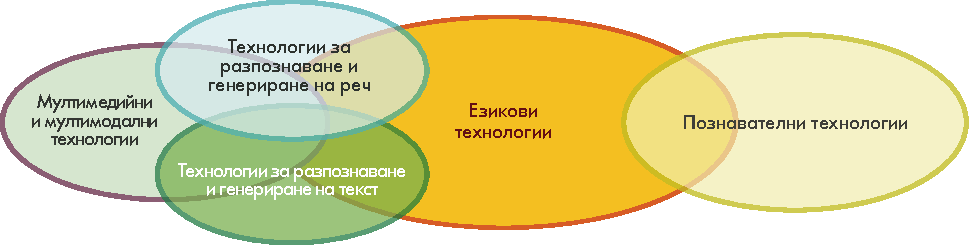
\includegraphics[width=\textwidth]{../_media/bulgarian/language_technologies}
  \caption{FIXME}
  \label{fig:ltincontext_de}
  \colorrule{grey3}{\textwidth}{1.5pt}
\end{figure*}

В тази глава  ще бъдат представени основните сфери на приложение на
езиковите технологии — проверка на правопис и граматика, търсене в
интернет, технологии за анализ и синтез на реч и машинен превод. Това
са приложения като: 

\begin{itemize}
\item проверка на правописа;
\item помощ при съставяне на текстове;
\item компютърно подпомогнато езиково обучение;
\item обработка на информация;
\item извличане на информация;
\item резюмиране на текст;
\item автоматично отговаряне на въпроси;
\item анализиране на реч;
\item синтезиране на реч.
\end{itemize}

Преди представянето на тези приложения, накратко ще бъде описана  архитектурата на типична система за езикова обработка.

\subsection{Архитектура на стандартна система за езикова обработка}

Софтуерните приложения за езикова обработка обикновено се състоят от няколко компонента, които съответстват на различни аспекти от езика. Фигурата представя силно опростена архитектура, която може да се срещне в стандартна система за обработка на текст. 

\begin{figure*}[b]
  \colorrule{grey3}{\textwidth}{1.5pt}
  \center
  %\vspace{-5mm} 
  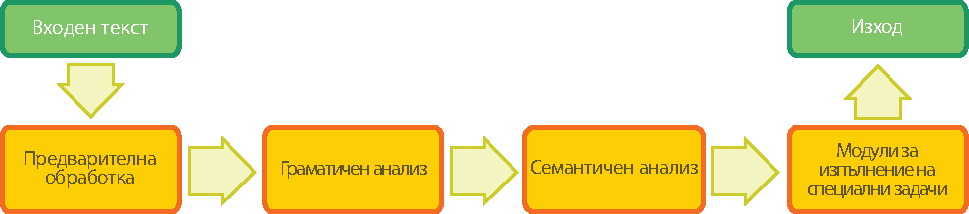
\includegraphics[width=\textwidth]{../_media/bulgarian/text_processing_app_architecture}
  \caption{Архитектурно приложение за предварителна обработка на текста}
  \label{fig:textprocessingarch_de}
  \colorrule{grey3}{\textwidth}{1.5pt}
\end{figure*}

Първите три модула отговарят за структурата и значението на входния
текст:

\begin{enumerate}
\item Предварителна обработка: изчистване на данните, анализ или отстраняване на форматиране, разпознаване на езика на входния текст и др. 
\item Граматически анализ: разпознаване на глагола, комплементите, модификаторите и други части на речта; разпознаване на изреченска структура. 
\item Семантичен анализ: отстраняване на многозначност (кое значение е правилно в даден контекст); разрешаване на анафора (кое местоимение към кое съществително се отнася в дадено изречение или текст) и заместващи изрази; представяне на семантиката на изречението във вид, подходящ за компютърна обработка. 
\end{enumerate}

След анализ на текста модулите със специфично предназначение изпълняват различни операции, например автоматично съставяне на резюме на текста и проверка в базата данни. Архитектурата е опростена и обобщена, но илюстрира в разбираем вид сложността на приложенията за езикова обработка. 

След представяне на областите на приложение на езиковите технологии накратко ще бъдат разгледани изследователската и образователната дейност в тази сфера, както и завършените и действащи изследователски програми. Предлага се  и експертна оценка на съществуващите основни езикови ресурси и програми за обработка на езика по критерии като достъпност, завършеност и качество. Приложението на езиковите технологии за български е обобщено в таблица.

\subsection{Основни сфери на приложение}

В тази част от документа се представят най-важните езикови ресурси и програми за тяхната обработка, базирани на езикови технологии, както и свързаните дейности в България. Програмите и ресурсите, които са \textbf{подчертани} в текста, фигурират в таблицата, приложена в края на тази глава.  

\subsubsection{Програми за проверка на езика}

Всеки, който познава програма за текстообработка като Microsoft Word, знае, че се използва приложение за проверка на правописа (spell checker), което подчертава правописните грешки и дава предложения за поправка. Първата програма за коригиране на правописа просто сравнява думите, които се срещат в текста, със списък от правилно изписани думи. 

Съвременните програми са много по-съвършени. Освен че използват
езиково зависими алгоритми за \textbf{анализ на текста}, те разпознават
морфологични грешки (например образуване на множествено число), а
някои разпознават и грешки в синтаксиса (например липсващ глагол или
неправилно съгласуване - {\it Тя *написахме
  писмото}). Най-разпространените приложения за проверка на правописа
обаче няма да открият грешките в следния текст \cite{zar1}: 

\begin{quote}
  I have a spelling checker,\\
  It came with my PC.\\
  It plane lee marks four my revue\\
  Miss steaks aye can knot sea.
\end{quote}

За разпознаване на този тип грешки е необходим анализ на контекста, например да се провери дали дадена дума започва с главна буква, или не, както в: 

\begin{quote}
  Тя живее в \textbf{Стара} Загора.\\
  Тя е \textbf{стара} жена.
\end{quote}

Подобни случаи изискват формулиране на езиково специфична \textbf{граматика} (граматически правила) или използване на статистически езикови модели. В последния случай моделите изчисляват вероятността дадена дума да се появи в определен контекст (между думи, които я предхождат и следхождат). 
Статистически езиков модел може да се конструира автоматично, като се използва информация за голямо количество достоверни езикови данни (т. нар. \textbf{текстов корпус}). Досега повечето разработки са създавани за английски. Резултатите обаче не са лесно приложими за български, който е с по-свободен словоред и по-богати флективни модели. 

Проверката на правописа не се ограничава само до текстообработващите програми; тя се прилага и в помощни системи за писане на ръководства и техническа документация, съставени по специални стандарти, описващи продукти на информационните технологии, здравеопазването, инженерния сектор и други. 
Поради опасения от недоволни клиенти за нанесени щети в резултат на неточни или неправилно разбрани инструкции, компаниите отделят все повече внимание на качеството на техническата документация, особено когато се стремят към международния пазар (чрез превод или локализиране на документите).
Напредъкът в обработката на естествения език доведе до разработване на помощен софтуер, който подпомага пишещите техническа документация с речник и синтактични структури, съобразени с определени правила и (фирмени) ограничения за употребата на термини. 

\begin{figure*}[htb]
  \colorrule{grey3}{\textwidth}{1.5pt}
  %\vspace{-9mm}
  \center
  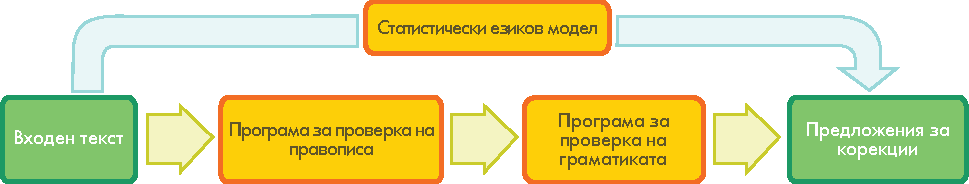
\includegraphics[width=\textwidth]{../_media/bulgarian/language_checking}
  \caption{Езикова проверка (вляво: основана на правила; вдясно: статистическа)}
  \label{fig:langcheckingaarch_de}
  \colorrule{grey3}{\textwidth}{1.5pt}
\end{figure*}

Освен програмите за проверка на правопис и помощните програми, приложенията за езикова проверка и корекция се използват и при компютърно подпомогнатото езиково обучение. Приложенията за проверка също така автоматично коригират заявки в уеб търсачките, например предложенията \textit{Did you mean...} на Google.

\subsubsection{Търсене в интернет}

Търсенето в мрежата, в интранет пространства или в дигитални библиотеки е вероятно най-широко използваното, но и най-недостатъчно развитото приложение на езиковите технологии днес. 
В момента търсачката Google, която се
 появява през 1998 г., се използва за около 80\% от всички търсения на информация в мрежата \cite{spi1}. 
%От 2004 г. думата {\it googeln} ({\it гуглирам}) дори е включена в речника Duden. 
Нито интерфейсът за търсене, нито този за
 намерените резултати са претърпели значителни
 промени. В настоящия си
 вид Google предлага корекция на правописа и
базови възможности за семантично търсене, което може да подобри
 точността чрез анализ на значението на
 термините в контекста на заявката  \cite{pc1}. Успехът на Google
 показва, че при наличието на голямо количество данни и ефективни
 техники за индексиране статистическите
 подходи постигат задоволителни резултати.

\begin{figure*}[htb]
  \colorrule{grey3}{\textwidth}{1.5pt}
  %\vspace{-9mm}
  \center
  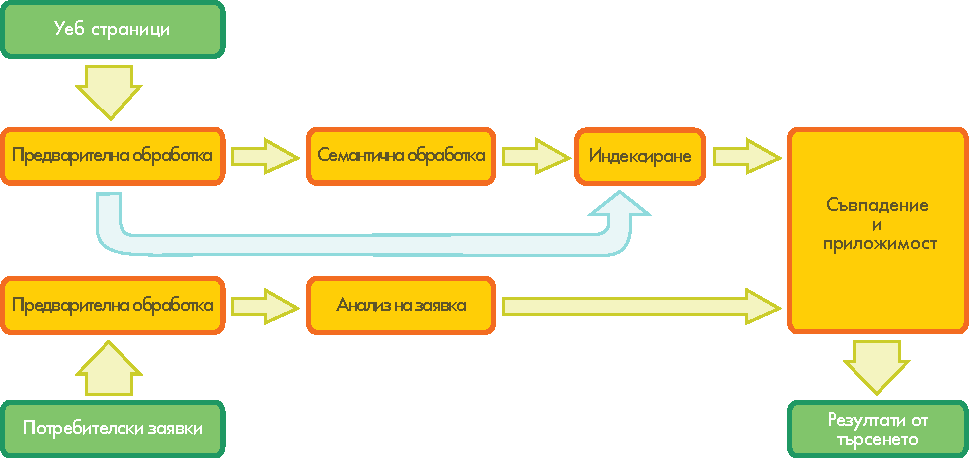
\includegraphics[width=\textwidth]{../_media/bulgarian/web_search_architecture}
  \vspace{-5mm}
  \caption{Архитектура за уеб търсене}
  \label{fig:websearcharch_de}
  \colorrule{grey3}{\textwidth}{1.5pt}
\end{figure*}

За по-детайлно търсене на информация обаче е нужно да
 се интегрира и значително лингвистично знание за \textbf{интерпретация на текста}. 
При изследвания, които използват \textbf{лексикални ресурси} като електронни тезауруси и онтологии (например WordNet за английски или еквивалента му за български BulNet), се наблюдава значителен напредък при откриване на уеб
 страници с помощта на синонимите на търсените думи или изрази, например {\it атомна енергия} и {\it ядрена енергия}, или дори с по-далечно свързани думи и изрази.

Следващото поколение търсачки трябва да се базира на
 по-развити езикови технологии, за да се справи със случаите, когато търсенето се състои от въпрос или друг вид изречение вместо от списък с ключови думи. 
 Например за заявката: \textit{Искам списъка на всички компании, които
 са били придобити от други компании през последните пет
 години}, системата трябва да анализира  изречението на синтактично и семантично равнище, като генерира индекс, който позволява бързото намиране на релевантни документи. Подходящият отговор ще изисква синтактичен анализ на граматическата структура на изречението, за да се определи, че потребителят търси компании, които са били придобити, а не компании, които са придобили
 други компании. За да се удовлетвори изразът \textit{последните пет години}, системата трябва да ограничи подходящия период. Заявката трябва да бъде съпоставена с голямо количество неструктурирани данни, за да се
 открие късчето или късчетата информация, които потребителят търси. Този процес се нарича „извличане на информация“ и включва търсене и оценяване на релевантността на  документите. За генерирането на списък от компании системата трябва да разпознае определена поредица от думи
 в документа като име на компания, процес, известен като „идентификация на
 именувани обекти“.

Още по-големи са предизвикателствата при опитите за разпознаване на търсения термин на даден език в документи на друг език. Междуезиковото извличане на информация включва автоматичен превод на заявката
 на всички участващи езици и превод на получената информация обратно на езика, на който е направена заявката.

Данните в нетекстови формати стават все повече и се увеличава необходимостта от услуги, които предоставят извличане на мултимедийна информация под
 формата на изображения, аудио и видео данни. При аудио и видео файловете се използва модул за разпознаване
 на реч, конвертиращ речта в текст (или във
 фонетична репрезентация), който може да бъде
 съпоставен със заявката на потребителя.
 
Някои български портали разполагат с crawler софтуер (т. нар.
 „паяк“), подобен на използвания от глобалните
 търсачки, който индексира сайтовете, класифицирани в
 категории. Например Dir.bg е един от първите и най-
големи уеб портали в България, който стартира
 автономна услуга – Diri.bg. „Дири“ е по-стара българска дума за „търси“. 

Технологиите с отворен код като
 Lucene и SOL често се използват от компании,
 разработващи софтуер за търсене, като базисна
 инфраструктура за търсачките. Други компании,
 работещи в областта, разчитат на технологии като FAST или Exalead.
Фокус на развитието е разработването на допълнителни приложения и ново поколение търсачки за специализирани портали, прилагайки технологии за семантичен анализ. Поради необходимостта от голяма процесорна мощ подобни търсещи машини са икономически оправдани само при обработване на сравнително малки текстове. Времето за обработка може да надмине в пъти това на традиционна статистическа търсачка, например Google. Такъв тип търсещи машини изискват разширено моделиране на тематично зависими данни, което ги прави нерентабилни за използв
 ане в интернет.

\subsubsection{Технологии за обработка на реч}

Технологиите за обработка на реч служат за създаването на интерфейс, който позволява на потребителя директна комуникация с машините, а не чрез графичен монитор, клавиатура и мишка. Днес подобен гласов
 потребителски интерфейс (Voice User Interface — VUI) се използва в приложения, осигуряващи частично или напълно
 автоматизирани гласови услуги, които компаниите предлагат на своите клиенти, служители или партньори
 по телефона. VUI е най-разпространен в банкирането, логистиката,
 обществения транспорт и телекомуникациите.
 Технологиите за гласова комуникация се използват и в интерфейса на вградени в колите системи за навигация, както и като алтернатива на потребителския
 интерфейс на смартфоните.

\begin{figure*}[htb]
  \colorrule{grey3}{\textwidth}{1.5pt}
  %\vspace{-9mm}
  \center  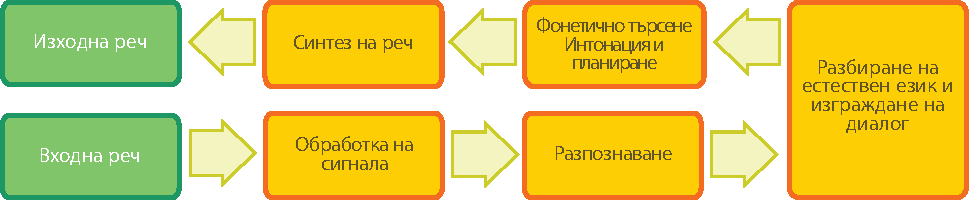
\includegraphics[width=\textwidth]{../_media/bulgarian/simple_speech-based_dialogue_architecture}
  \center
  \caption{Проста диалогова архитектура, базирана на реч}
  \label{fig:dialoguearch_de}
  \colorrule{grey3}{\textwidth}{1.5pt}
\end{figure*}

Технологиите за гласова комуникация включват четири различни модула:

\begin{enumerate}
\item Автоматичното \textbf{разпознаване на реч}  (automatic speech recognition — ASR)  идентифицира изречените думите в поредицата от звукове, произнесени от потребителя.
\item Разбирането на речта на потребителя включва анализ на синтактичната структура и семантична интерпретация  на изказването.
\item Диалоговият мениджмънт определя какви действия ще се предприемат въз основа на входните данни и функционалността на системата.
\item Технологията за \textbf{синтезиране на реч}, превръщане на текст в
 реч (text-to-speech — TTS), трансформира отговора на системата в
 звукове, изходни данни към потребителя.
\end{enumerate}

Едно от основните предизвикателства е разработването на ASR система, която разпознава произнесените думи колкото е възможно по-точно. Това изисква или
 ограничение на речта на потребителите до определено множество от ключови думи, или ръчно създаване на езикови модели, които покриват
в значителна степен възможния изговор на носителите на езика.
С техниките за машинно самообучение езиковите модели могат да бъдат автоматично генерирани от \textbf{корпуси с реч} — големи колекции от аудио файлове или транскрибирана реч.
Ограничението в броя на изказванията обикновено затруднява  използването на VUI  и влошава възприемането. От друга страна, създаването, настройването и поддържането на богати  езикови модели увеличава разходите.
 
Гласови интерфейси, които се базират на езикови модели и позволяват на потребителя да се изразява сравнително свободно, подпомаган от изрази като \textit{Как мога да Ви помогна?}, постепенно се автоматизират и се възприемат по-добре от потребителите.
При генерирането на автоматичен отговор при гласовата комуникация компаниите използват предварително записани фрази, изречени от професионални говорители. Подобен подход е подходящ при статични изказвания, при които произношението не зависи от контекста или потребителя. При по-динамично съдържание може да се получи неестествена интонация, тъй като  малки части от аудио файлове просто се наслагват една след друга. Съвременните TTS системи са доста по-добри (макар че и при тях  има поле за развитие) по отношение на естественото звучене 
 на динамичните изказвания.

През последното десетилетие технологиите при отделните компоненти за гласовата комуникация са стандартизирани в значителна степен. Наблюдава се пазарна консолидация в сферата на разпознаване и генериране на реч. В този сектор националните пазари на икономически силните и гъсто населени страни от Г-20 се доминират от по-малко от пет компании, сред които водещи в Европа са американската Nuance и италианската Loquendo. Поредната стъпка към по-сериозна пазарна консолидация  е придобиването на Loquendo от Nuance през 2011 г.

На българския TTS пазар се предлагат много ограничен брой програми за синтезиране на реч. Например SpeechLab 2.0 се разпространява свободно за хора със зрителни проблеми. „Сиела“, издателство за юридическа литература, е разработила система за разпознаване на българска реч. В областта на  гласовата комуникация все още няма развит пазар за ключовите технологии, базирани на синтактичен и семантичен анализ.
Употребата на VUI в България има тенденция към увеличение през последните пет години. За това играе роля повишеното търсене на системи за автоматично
 обслужване на потребителите, оптимизацията на
 разходите при автоматизираните телефонни услуги и
 нарасналото използване на речта при комуникацията между човек и
машина.

В бъдеще вероятно ще настъпят значителни промени в
 резултат на разпространението на смартфоните като
 нова платформа за контакти (освен телефоните, интернет и имейл).
Тази тенденция ще се отрази и при технологиите за
 гласова комуникация. Търсенето на
 телефонно базирани VUI ще намалее в дългосрочен
 план, а удобното за потребителите използване на гласова комуникация ще придобива все по-голямо значение при смартфоните. Наблюдава се подобрение на
 точността при разпознаването на реч, независимо от особеностите на
 говорещия, в услугите за гласови указания, които вече се предлагат от централите за обслужване на смартфон.

\subsubsection{Машинен превод}

Идеята за използване на компютрите за превод
 на естествен език се появява още през 1946 г.,
 задачата получава значително финансиране през 50-те години и отново през 80-те години на 20-ти век. \textbf{Машинният превод} (МТ) обаче все още не успява да оправдае надеждите за качествен автоматизиран превод, съпътстващи го от раждането му.
В първата си фаза технологиите за MT просто заменят думи от един естествен език с думи от друг. Това може да
 е приемливо в определени жанрове със стандартизиран език и повторение на формулировки, например прогнозите за времето.
 За добър превод на произволни текстове обаче
 по-големи  сегменти (фрази, изречения и дори цели параграфи) трябва да се съотнесат максимално точно с най-близките им паралели на другия
 език. Основната трудност се крие във факта, че
 човешкият език се характеризира с многозначност на 
всички равнища,
 например
 многозначност на лексикално ниво ({\it ягуар} – животно
 или модел кола) или на
 синтактично ниво, както в:

\begin{itemize}
\item Полицаят наблюдава престъпника с телескопа.
\item Полицаят наблюдава престъпника с пистолета.
\end{itemize}

Един от подходите се основава на лингвистични правила.
 При близки езици прекият превод дума по дума може да е приемлив в някои случаи. Често обаче системите,
 базирани на правила (или основани на лингвистични знания),
 анализират входния текст и създават преходна, символна
 репрезентация, от която се генерира текстът в
 производния език. Успехът на този метод зависи от
 достъпа до богати речници с морфологична, синтактична
 и семантична информация, както и от наличието на
 богат набор от граматически правила, създадени от лингвисти.
 Това е дълъг процес, свързан със значителни разходи.

\begin{figure*}[htb]
  \colorrule{grey3}{\textwidth}{1.5pt}
  %\vspace{-21mm}
  \center
  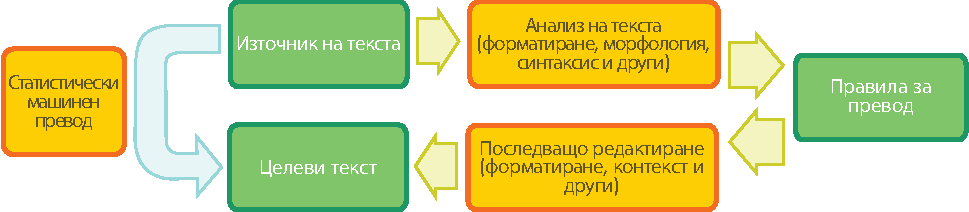
\includegraphics[width=\textwidth]{../_media/bulgarian/machine_translation}
  \vspace{-2mm}
  \caption{Машинен превод (отгоре: статистически; отдолу: базиран на правила)}
  \label{fig:mtarch_de}
  \colorrule{grey3}{\textwidth}{1.5pt}
\end{figure*}

От края на 80-те години на миналия век компютрите стават все по-мощни, както и по-евтини, затова интересът към статистическите модели за машинен превод се засилва. Статистическите модели се извличат
 след анализ на двуезични текстови корпуси като
 паралелния корпус Europarl със стенограми на
 Европейския парламент на 11 европейски езика. При наличието на достатъчно данни статистическият машинен превод е сравнително добър при представянето на значението на изходния текст, като обработва паралелни текстове и намира съответстващи си последователности от думи. За разлика от базираните на лингвистично знание системи статистическият (основаващ се на данни) машинен превод често генерира неграматичен текст. Положителното е, че се изисква по-малко човешки труд и се откриват на някои специфични лингвистични явления (например ид�
 �оми), които трудно се предават с лингвистични правила. 

Силните и слабите места на двата метода (статистически и лингвистичен) се компенсират взаимно, така че изследователите се насочват към
 хибридни подходи, които комбинират решения от двата модела по различни начини. Възможно е да се използват едновременно системи, основани на данни, и
 такива, основани на правила, и да се изработи модул за избор, който преценява кой е най-добрият преводен резултат за всяко изречение. 

При изречения с повече от 12 думи обаче резултатът често не е задоволителен. По-добро решение е да се комбинират най-добре преведените части в рамките на всяко изречение, избрани сред множеството от предложени алтернативи. 
Задачата е доста сложна, тъй като съответстващите си части в рамките на дадено множество невинаги са очевидни.

Машинният превод за българския език е още по-голямо предизвикателство. Проблемите са свързани с феномени като липсата на падежно окончание при имената, сравнително свободния словоред и незадължително изразения подлог. Богатата морфология при глаголите допълнително затруднява генерирането на думи с подходящите граматически характеристики.

Един от успешните примери за български е WebTrance на SkayCode – система за машинен превод, която автоматично превежда текстове, помощни файлове, менюта и интернет страници от английски, немски, френски, испански, италиански и турски на и от български. Ако се използва и програма, която се съобразява със специфичната терминология, машинният превод може значително да увеличи продуктивността при превода.

Все  още има голям потенциал при подобряването на качеството на системите за машинен превод. Трудностите са свързани с адаптация на езиковите ресурси към определена тематична или потребителска област и интеграция на технологията в
 съществуващи системи, които са терминологично базирани и използват преводна памет. 

Повечето познати системи са изградени около и/или са насочени към английски език и поддържат превод от и на малко езици спрямо български. Липсва унификация, така че се налага потребителите на машинен превод да усвоят
 различни методи при използването на допълнителни речници за различните системи.

При оценка на качеството се сравнява работата на системите за
 машинен превод, ефективността на подходите и статусът на превода за отделни
 езикови двойки. В таблицата, разработена по европейския проект
 Euromatrix+, са представени резултатите от машинния
 превод между езикови двойки за 22 от 23-те официални езика на ЕС
 (без ирландски), изчислени по точковата система BLEU, която оценява с повече точки по-добрия превод \cite{bleu1}. (Професионален преводач би получил около 80 точки.)

Най-добри резултати (в зелено и синьо) са за езици, които са били обект на значителни изследователски усилия в координирани програми и са представени в големи по обем паралелни корпуси (английски, френски, холандски, испански и немски). С най-слаби резултати (в червено) са езиците, които не са били обект на проекти и проучвания, или такива, които структурно се различават в значителна степен от останалите езици (унгарски, малтийски, фински).


\begin{figure*}[tb]
  \centering
  \setlength{\tabcolsep}{0.17em}
  \small
  \begin{tabular}{>{\columncolor{corange1}}cccccccccccccccccccccccc}
    & \multicolumn{22}{>{\columncolor{corange1}}c}{Език цел -- \textcolor{grey1}{Target language}}\\\addlinespace[{-.009cm}]
    \rowcolor{corange1}  & EN & BG & DE & CS & DA & EL & ES & ET & FI & FR & HU & IT & LT & LV & MT & NL & PL & PT & RO & SK & SL & SV\\
    EN & -- & \textcolor{blue}{40.5} & \textcolor{blue}{46.8} & \textcolor{green2}{52.6} & \textcolor{green2}{50.0} & \textcolor{blue}{41.0} & \textcolor{green2}{55.2} & \textcolor{purple}{34.8} & \textcolor{purple}{38.6} & \textcolor{green2}{50.1} & \textcolor{purple}{37.2} & \textcolor{green2}{50.4} & \textcolor{purple}{39.6} & \textcolor{blue}{43.4} & \textcolor{purple}{39.8} & \textcolor{green2}{52.3} & \textcolor{blue}{49.2} & \textcolor{green2}{55.0} & \textcolor{blue}{49.0} & \textcolor{blue}{44.7} & \textcolor{green2}{50.7} & \textcolor{green2}{52.0}\\
    BG & \textcolor{green}{61.3} & -- & \textcolor{purple}{38.7} & \textcolor{purple}{39.4} & \textcolor{purple}{39.6} & \textcolor{purple}{34.5} & \textcolor{blue}{46.9} & \textcolor{red3}{25.5} & \textcolor{red3}{26.7} & \textcolor{blue}{42.4} & \textcolor{red3}{22.0} & \textcolor{blue}{43.5} & \textcolor{red3}{29.3} & \textcolor{red3}{29.1} & \textcolor{red3}{25.9} & \textcolor{blue}{44.9} & \textcolor{purple}{35.1} & \textcolor{blue}{45.9} & \textcolor{purple}{36.8} & \textcolor{purple}{34.1} & \textcolor{purple}{34.1} & \textcolor{purple}{39.9}\\
    DE & \textcolor{green2}{53.6} & \textcolor{red3}{26.3} & -- & \textcolor{purple}{35.4} & \textcolor{blue}{43.1} & \textcolor{purple}{32.8} & \textcolor{blue}{47.1} & \textcolor{red3}{26.7} & \textcolor{red3}{29.5} & \textcolor{purple}{39.4} & \textcolor{red3}{27.6} & \textcolor{blue}{42.7} & \textcolor{red3}{27.6} & \textcolor{purple}{30.3} & \textcolor{red2}{19.8} & \textcolor{green2}{50.2} & \textcolor{purple}{30.2} & \textcolor{blue}{44.1} & \textcolor{purple}{30.7} & \textcolor{red3}{29.4} & \textcolor{purple}{31.4} & \textcolor{blue}{41.2}\\
    CS & \textcolor{green2}{58.4} & \textcolor{purple}{32.0} & \textcolor{blue}{42.6} & -- & \textcolor{blue}{43.6} & \textcolor{purple}{34.6} & \textcolor{blue}{48.9} & \textcolor{purple}{30.7} & \textcolor{purple}{30.5} & \textcolor{blue}{41.6} & \textcolor{red3}{27.4} & \textcolor{blue}{44.3} & \textcolor{purple}{34.5} & \textcolor{purple}{35.8} & \textcolor{red3}{26.3} & \textcolor{blue}{46.5} & \textcolor{purple}{39.2} & \textcolor{blue}{45.7} & \textcolor{purple}{36.5} & \textcolor{blue}{43.6} & \textcolor{blue}{41.3} & \textcolor{blue}{42.9}\\
    DA & \textcolor{green2}{57.6} & \textcolor{red3}{28.7} & \textcolor{blue}{44.1} & \textcolor{purple}{35.7} & -- & \textcolor{purple}{34.3} & \textcolor{blue}{47.5} & \textcolor{red3}{27.8} & \textcolor{purple}{31.6} & \textcolor{blue}{41.3} & \textcolor{red3}{24.2} & \textcolor{blue}{43.8} & \textcolor{red3}{29.7} & \textcolor{purple}{32.9} & \textcolor{red3}{21.1} & \textcolor{blue}{48.5} & \textcolor{purple}{34.3} & \textcolor{blue}{45.4} & \textcolor{purple}{33.9} & \textcolor{purple}{33.0} & \textcolor{purple}{36.2} & \textcolor{blue}{47.2}\\
    EL & \textcolor{green2}{59.5} & \textcolor{purple}{32.4} & \textcolor{blue}{43.1} & \textcolor{purple}{37.7} & \textcolor{blue}{44.5} & -- & \textcolor{green2}{54.0} & \textcolor{red3}{26.5} & \textcolor{red3}{29.0} & \textcolor{blue}{48.3} & \textcolor{red3}{23.7} & \textcolor{blue}{49.6} & \textcolor{red3}{29.0} & \textcolor{purple}{32.6} & \textcolor{red3}{23.8} & \textcolor{blue}{48.9} & \textcolor{purple}{34.2} & \textcolor{green2}{52.5} & \textcolor{purple}{37.2} & \textcolor{purple}{33.1} & \textcolor{purple}{36.3} & \textcolor{blue}{43.3}\\
    ES & \textcolor{green}{60.0} & \textcolor{purple}{31.1} & \textcolor{blue}{42.7} & \textcolor{purple}{37.5} & \textcolor{blue}{44.4} & \textcolor{purple}{39.4} & -- & \textcolor{red3}{25.4} & \textcolor{red3}{28.5} & \textcolor{green2}{51.3} & \textcolor{red3}{24.0} & \textcolor{green2}{51.7} & \textcolor{red3}{26.8} & \textcolor{purple}{30.5} & \textcolor{red3}{24.6} & \textcolor{blue}{48.8} & \textcolor{purple}{33.9} & \textcolor{green2}{57.3} & \textcolor{purple}{38.1} & \textcolor{purple}{31.7} & \textcolor{purple}{33.9} & \textcolor{blue}{43.7}\\
    ET & \textcolor{green2}{52.0} & \textcolor{red3}{24.6} & \textcolor{purple}{37.3} & \textcolor{purple}{35.2} & \textcolor{purple}{37.8} & \textcolor{red3}{28.2} & \textcolor{blue}{40.4} & -- & \textcolor{purple}{37.7} & \textcolor{purple}{33.4} & \textcolor{purple}{30.9} & \textcolor{purple}{37.0} & \textcolor{purple}{35.0} & \textcolor{purple}{36.9} & \textcolor{red3}{20.5} & \textcolor{blue}{41.3} & \textcolor{purple}{32.0} & \textcolor{purple}{37.8} & \textcolor{red3}{28.0} & \textcolor{purple}{30.6} & \textcolor{purple}{32.9} & \textcolor{purple}{37.3}\\
    FI & \textcolor{blue}{49.3} & \textcolor{red3}{23.2} & \textcolor{purple}{36.0} & \textcolor{purple}{32.0} & \textcolor{purple}{37.9} & \textcolor{red3}{27.2} & \textcolor{purple}{39.7} & \textcolor{purple}{34.9} & -- & \textcolor{red3}{29.5} & \textcolor{red3}{27.2} & \textcolor{purple}{36.6} & \textcolor{purple}{30.5} & \textcolor{purple}{32.5} & \textcolor{red2}{19.4} & \textcolor{blue}{40.6} & \textcolor{red3}{28.8} & \textcolor{purple}{37.5} & \textcolor{red3}{26.5} & \textcolor{red3}{27.3} & \textcolor{red3}{28.2} & \textcolor{purple}{37.6}\\
    FR & \textcolor{green}{64.0} & \textcolor{purple}{34.5} & \textcolor{blue}{45.1} & \textcolor{purple}{39.5} & \textcolor{blue}{47.4} & \textcolor{blue}{42.8} & \textcolor{green}{60.9} & \textcolor{red3}{26.7} & \textcolor{purple}{30.0} & -- & \textcolor{red3}{25.5} & \textcolor{green2}{56.1} & \textcolor{red3}{28.3} & \textcolor{purple}{31.9} & \textcolor{red3}{25.3} & \textcolor{green2}{51.6} & \textcolor{purple}{35.7} & \textcolor{green}{61.0} & \textcolor{blue}{43.8} & \textcolor{purple}{33.1} & \textcolor{purple}{35.6} & \textcolor{blue}{45.8}\\
    HU & \textcolor{blue}{48.0} & \textcolor{red3}{24.7} & \textcolor{purple}{34.3} & \textcolor{purple}{30.0} & \textcolor{purple}{33.0} & \textcolor{red3}{25.5} & \textcolor{purple}{34.1} & \textcolor{red3}{29.6} & \textcolor{red3}{29.4} & \textcolor{purple}{30.7} & -- & \textcolor{purple}{33.5} & \textcolor{red3}{29.6} & \textcolor{purple}{31.9} & \textcolor{red2}{18.1} & \textcolor{purple}{36.1} & \textcolor{red3}{29.8} & \textcolor{purple}{34.2} & \textcolor{red3}{25.7} & \textcolor{red3}{25.6} & \textcolor{red3}{28.2} & \textcolor{purple}{30.5}\\
    IT & \textcolor{green}{61.0} & \textcolor{purple}{32.1} & \textcolor{blue}{44.3} & \textcolor{purple}{38.9} & \textcolor{blue}{45.8} & \textcolor{blue}{40.6} & \textcolor{red3}{26.9} & \textcolor{red3}{25.0} & \textcolor{red3}{29.7} & \textcolor{green2}{52.7} & \textcolor{red3}{24.2} & -- & \textcolor{red3}{29.4} & \textcolor{purple}{32.6} & \textcolor{red3}{24.6} & \textcolor{green2}{50.5} & \textcolor{purple}{35.2} & \textcolor{green2}{56.5} & \textcolor{purple}{39.3} & \textcolor{purple}{32.5} & \textcolor{purple}{34.7} & \textcolor{blue}{44.3}\\
    LT & \textcolor{green2}{51.8} & \textcolor{red3}{27.6} & \textcolor{purple}{33.9} & \textcolor{purple}{37.0} & \textcolor{purple}{36.8} & \textcolor{red3}{26.5} & \textcolor{red3}{21.1} & \textcolor{purple}{34.2} & \textcolor{purple}{32.0} & \textcolor{purple}{34.4} & \textcolor{red3}{28.5} & \textcolor{purple}{36.8} & -- & \textcolor{blue}{40.1} & \textcolor{red3}{22.2} & \textcolor{purple}{38.1} & \textcolor{purple}{31.6} & \textcolor{purple}{31.6} & \textcolor{red3}{29.3} & \textcolor{purple}{31.8} & \textcolor{purple}{35.3} & \textcolor{purple}{35.3}\\
    LV & \textcolor{green2}{54.0} & \textcolor{red3}{29.1} & \textcolor{purple}{35.0} & \textcolor{purple}{37.8} & \textcolor{purple}{38.5} & \textcolor{red3}{29.7} & \textcolor{red2}{8.0} & \textcolor{purple}{34.2} & \textcolor{purple}{32.4} & \textcolor{purple}{35.6} & \textcolor{red3}{29.3} & \textcolor{purple}{38.9} & \textcolor{purple}{38.4} & -- & \textcolor{red3}{23.3} & \textcolor{blue}{41.5} & \textcolor{purple}{34.4} & \textcolor{purple}{39.6} & \textcolor{purple}{31.0} & \textcolor{purple}{33.3} & \textcolor{purple}{37.1} & \textcolor{purple}{38.0}\\
    MT & \textcolor{green}{72.1} & \textcolor{purple}{32.2} & \textcolor{purple}{37.2} & \textcolor{purple}{37.9} & \textcolor{purple}{38.9} & \textcolor{purple}{33.7} & \textcolor{blue}{48.7} & \textcolor{red3}{26.9} & \textcolor{red3}{25.8} & \textcolor{blue}{42.4} & \textcolor{red3}{22.4} & \textcolor{blue}{43.7} & \textcolor{purple}{30.2} & \textcolor{purple}{33.2} & -- & \textcolor{blue}{44.0} & \textcolor{purple}{37.1} & \textcolor{blue}{45.9} & \textcolor{purple}{38.9} & \textcolor{purple}{35.8} & \textcolor{blue}{40.0} & \textcolor{blue}{41.6}\\
    NL & \textcolor{green2}{56.9} & \textcolor{red3}{29.3} & \textcolor{blue}{46.9} & \textcolor{purple}{37.0} & \textcolor{blue}{45.4} & \textcolor{purple}{35.3} & \textcolor{blue}{49.7} & \textcolor{red3}{27.5} & \textcolor{red3}{29.8} & \textcolor{blue}{43.4} & \textcolor{red3}{25.3} & \textcolor{blue}{44.5} & \textcolor{red3}{28.6} & \textcolor{purple}{31.7} & \textcolor{red3}{22.0} & -- & \textcolor{purple}{32.0} & \textcolor{blue}{47.7} & \textcolor{purple}{33.0} & \textcolor{purple}{30.1} & \textcolor{purple}{34.6} & \textcolor{blue}{43.6}\\
    PL & \textcolor{green}{60.8} & \textcolor{purple}{31.5} & \textcolor{blue}{40.2} & \textcolor{blue}{44.2} & \textcolor{blue}{42.1} & \textcolor{purple}{34.2} & \textcolor{blue}{46.2} & \textcolor{red3}{29.2} & \textcolor{red3}{29.0} & \textcolor{blue}{40.0} & \textcolor{red3}{24.5} & \textcolor{blue}{43.2} & \textcolor{purple}{33.2} & \textcolor{purple}{35.6} & \textcolor{red3}{27.9} & \textcolor{blue}{44.8} & -- & \textcolor{blue}{44.1} & \textcolor{purple}{38.2} & \textcolor{purple}{38.2} & \textcolor{purple}{39.8} & \textcolor{blue}{42.1}\\
    PT & \textcolor{green}{60.7} & \textcolor{purple}{31.4} & \textcolor{blue}{42.9} & \textcolor{purple}{38.4} & \textcolor{blue}{42.8} & \textcolor{blue}{40.2} & \textcolor{green}{60.7} & \textcolor{red3}{26.4} & \textcolor{red3}{29.2} & \textcolor{green2}{53.2} & \textcolor{red3}{23.8} & \textcolor{green2}{52.8} & \textcolor{red3}{28.0} & \textcolor{purple}{31.5} & \textcolor{red3}{24.8} & \textcolor{blue}{49.3} & \textcolor{purple}{34.5} & -- & \textcolor{purple}{39.4} & \textcolor{purple}{32.1} & \textcolor{purple}{34.4} & \textcolor{blue}{43.9}\\
    RO & \textcolor{green}{60.8} & \textcolor{purple}{33.1} & \textcolor{purple}{38.5} & \textcolor{purple}{37.8} & \textcolor{blue}{40.3} & \textcolor{purple}{35.6} & \textcolor{green2}{50.4} & \textcolor{red3}{24.6} & \textcolor{red3}{26.2} & \textcolor{blue}{46.5} & \textcolor{red3}{25.0} & \textcolor{blue}{44.8} & \textcolor{red3}{28.4} & \textcolor{red3}{29.9} & \textcolor{red3}{28.7} & \textcolor{blue}{43.0} & \textcolor{purple}{35.8} & \textcolor{blue}{48.5} & -- & \textcolor{purple}{31.5} & \textcolor{purple}{35.1} & \textcolor{purple}{39.4}\\
    SK & \textcolor{green}{60.8} & \textcolor{purple}{32.6} & \textcolor{purple}{39.4} & \textcolor{blue}{48.1} & \textcolor{blue}{41.0} & \textcolor{purple}{33.3} & \textcolor{blue}{46.2} & \textcolor{red3}{29.8} & \textcolor{red3}{28.4} & \textcolor{purple}{39.4} & \textcolor{red3}{27.4} & \textcolor{blue}{41.8} & \textcolor{purple}{33.8} & \textcolor{purple}{36.7} & \textcolor{red3}{28.5} & \textcolor{blue}{44.4} & \textcolor{purple}{39.0} & \textcolor{blue}{43.3} & \textcolor{purple}{35.3} & -- & \textcolor{blue}{42.6} & \textcolor{blue}{41.8}\\
    SL & \textcolor{green}{61.0} & \textcolor{purple}{33.1} & \textcolor{purple}{37.9} & \textcolor{blue}{43.5} & \textcolor{blue}{42.6} & \textcolor{purple}{34.0} & \textcolor{blue}{47.0} & \textcolor{purple}{31.1} & \textcolor{red3}{28.8} & \textcolor{purple}{38.2} & \textcolor{red3}{25.7} & \textcolor{blue}{42.3} & \textcolor{purple}{34.6} & \textcolor{purple}{37.3} & \textcolor{purple}{30.0} & \textcolor{blue}{45.9} & \textcolor{purple}{38.2} & \textcolor{blue}{44.1} & \textcolor{purple}{35.8} & \textcolor{purple}{38.9} & -- & \textcolor{blue}{42.7}\\
    SV & \textcolor{green2}{58.5} & \textcolor{red3}{26.9} & \textcolor{blue}{41.0} & \textcolor{purple}{35.6} & \textcolor{blue}{46.6} & \textcolor{purple}{33.3} & \textcolor{blue}{46.6} & \textcolor{red3}{27.4} & \textcolor{purple}{30.9} & \textcolor{purple}{38.9} & \textcolor{red3}{22.7} & \textcolor{blue}{42.0} & \textcolor{red3}{28.2} & \textcolor{purple}{31.0} & \textcolor{red3}{23.7} & \textcolor{blue}{45.6} & \textcolor{purple}{32.2} & \textcolor{blue}{44.2} & \textcolor{purple}{32.7} & \textcolor{purple}{31.3} & \textcolor{purple}{33.5} & --\\
    \end{tabular}
  \caption{Резултати от машинния превод между 22 европейски езика  в проекта Euromatrix+ -- \textcolor{grey1}{Machine translation between 22 EU-languages \cite{euro1}}}
  \label{fig:euromatrix_de}
\end{figure*}

\subsection{Други сфери на приложение}

Изграждането на приложения, базирани на езикови технологии, включва редица задачи, които не винаги са видими при взаимодействието с потребителя,
 но предлагат важни функционалности в рамките на цялата система. Те са се развили до отделни поддисциплини на компютърната лингвистика.

Автоматичното отговоряне на въпроси например е област, на която се отделя все повече внимание и за която се изграждат анотирани корпуси и се организират изследователски състезания. Идеята е да се премине от търсене по ключови думи (при което програмите за търсене намират цяла колекция от потенциално
 подходящи документи) към сценарии, където потребителят задава конкретен въпрос и получава един отговор. Например: 
\begin{itemize}
\item[] Въпрос: {\it На каква възраст е бил Нийл Армстронг, когато е стъпил на Луната?}
\item[] Отговор: {\it 38.}
\end{itemize}

Автоматичното отговаряне на въпроси е свързано не само с търсенето в интернет, това е цяла изследователска област, която се занимава с множество проблеми, например: какви са типовете въпроси и как трябва да се обработват; как трябва да се анализират и сравнят множеството от документи, потенциално
 съдържащи отговора (дали отговорите не си противоречат); как
дадена информация (отговорът) може да бъде извлечена  надеждно от документа, без да се пренебрегва контекстът.
Това на свой ред е свързано със задачата за извличане на информация (information extraction — IE), която бе доста популярна в периода на „статистическата революция“ в компютърната лингвистика в началото на 90-те години. Извличането на информация има за цел да разпознае специфична информация от определени класове документи, например разпознаване на ключовите играчи при
 придобиване на компании според материали в медиите. Друг сценарий е свързан с новините за терористични инциденти, в които задачата е текстът да се съпостави  с модел, в който се определят извършителят, целта, времето, мястото и резултатът от инцидента. Попълването на модела, специфично за дадена тематична област, е най-важният етап при извличането на информация – още
 един пример за добре насочена изследователска област към практически цели, която впоследствие трябва да бъде внедрена в подходящи приложения.

Две гранични области, които понякога се определят като автономни приложения, а понякога са част от друга услуга, са резюмирането и генерирането на текст. 

При резюмирането се създава кратко обобщение на по-дълъг текст. Приложение за резюмиране е вградено и в Microsoft Word. Тази задача се основава предимно на статистически данни - идентифицират се „важните“ думи в даден текст (тоест, думите, които са най-често срещани, но все
 пак по-рядко, отколкото в текстове с обща употреба) и
 след това се определят онези изречения, които съдържат
 голямо количество „важни“ думи. Тези изречения се извличат от документа и образуват резюмето. В този разпространен сценарий резюмирането е равносилно на извличане на изречения: текстът се редуцира до част от изреченията си.
 Алтернативният подход включва синтезиране на нови
 изречения, които не са извлечени от изходния текст. Този подход изисква дълбок семантичен анализ на текста и е по-неясен. Генерирането на текст в повечето случаи не е автономно приложение, а е интегрирано в по-голяма софтуерна среда, например в медицински информационни системи, където се събират, съхраняват и обработват данни за пациентите - генерирането на информационна справка е само едно от многото възможни приложения.
 
Всички тези технологии са доста по-слабо развити за български, отколкото за английски, където отговорянето на въпроси, извличането на информация
 и резюмирането на текст са били обект на множество конкурентни проекти и най-вече на инициативи, организирани в САЩ от 90-те години насам от правителствено спонсорираните организации DAPRA и INST. Така развитието в областта се подобрява значително, но фокусът винаги е бил върху английски. По тази причина няма анотирани корпуси и други специализирани ресурси за български. Трябва да се отбележи обаче, че системите за резюмиране, основани на статистически методи, често са до известна степен езиково независими, а някои изследователски прототи�
 �и се предлагат и на пазара.

При генериране на текст компонентите за многократно приложение обикновено са
 ограничени до модули за повърхнинно генериране (т. нар. генериращи граматики). И тук по-голяма част от наличния софтуер е предназначен за английски език.

\subsection{Образователни програми за езикови технологии}

Езиковите технологии са интердисциплинарна област, която разчита на висококвалифицирания труд на лингвисти, програмисти, математици, философи, психолингвисти и невролози. Необходимостта от експертно знание и ресурси е и една от пречките пред утвърждаването на езиковите технологии сред задължителните образователни програми в България. 
Българските университети предлагат ограничени възможности за специализирано
 обучение в областта на компютърната лингвистика.
 Курсовете и програмите са насочени или
 към студенти в областта на хуманитарните науки, или
 към математици, но не покриват нуждите и на двете
 групи специалисти. Преди две години Пловдивският университет откри бакалавърска програма
 по лингвистика и информационни технологии. През
 учебната 2009/10 г. за тази програма се записаха 30
 студенти, а през следващата броят на желаещите се
 удвои. На студентите се предлага широк набор от курсове
 по
 основи
 на
 лингвистиката, математика
 и
 програмиране, както и възможности за запознаване и
 работа с приложенията за езикови технологии.
 Бакалавърската
 програма
 по
 информатика
 в
 Пловдивския университет по традиция предлага
 лекционен курс по компютърна лингвистика.

От 2004 г. Факултетът по математика и информатика към Софийския университет поддържа магистърска програма
 по
 изкуствен
 интелект.
 Софийският университет предлага и магистърска програма по компютърна лингвистика, в която са включени курсове в
 областта на математика, логиката, програмирането и
 теоретичната лингвистика. Дипломантите на тези програми получават добро
 обучение за започване на научна и академична кариера,
 както и по-обща теоретична и компютърна грамотност,
 която им позволява да работят по изграждането на
 неконвенционални практически приложения. За успеха
 на програмите може да се съди по професионалното
 развитие на завършилите ги, които работят във водещи
 технологични и компютърни компании, национални и
 специализирани медии и научни и академични
 институции.
Обучението на достатъчен брой специалисти в областта на езиковите технологии е предпоставка за развитието на научните изследвания и следователно за успешни комерсиални приложения. 

\subsection{Национални проекти и инициативи}

Първите проекти за създаване на езикови
 технологии с международно и национално финансиране
 се появяват в началото на 90-те години на миналия
 век. За кратък период от време редица научни проекти
 получават финансиране от европейските институции.
 Сред тях са: LaTeSLav (Language Processing Technologies for Slavic Languages, 1991-1994), който има за цел
 създаване на прототип на програма за граматична
 корекция; BILEDITA (Bilingual Electronic Dictionaries and Intelligent Text Alignment, 1996-1998) – за създаване на
 двуезични електронни речници; GLOSSER (Support of Second Language Acquisition and Learning from Aligned Corpora, 1996-1998)
 – в подкрепа на обучението по чужди езици и други
 образователни цели. Multext-East (Multilingual Text Tools and Corpora for Central and Eastern European Languages, 1995-1997) е
 продължение на предходните проекти Multext и EAGLES (European Commission's Expert Advisory Group on Language Engineering Standards), който предлага ресурси със стандартно маркиране
 и анотация за български
и други европейски езици. По-късно ресурсите са разширени и допълнени по проектите ELAN (European Languagе Activity Network, 1998-1999), TELRI, фази I и II (TransEuropean Language Resources Infrastructure 1995-1998 /
1999-2001); и Concede (Consortium for Central European
 Dictionary Encoding, 1998-2000).

Националният фонд „Научни изследвания“ към Министерството на образованието, младежта и науката
 подкрепя научните изследвания чрез редица програми
 за финансиране на национално равнище. По този начин се подпомагат редица изследователски проекти, сътрудничеството с международни изследователски
 центрове и компании и се изгражда основата
 за технологично развитие и комерсиални приложения за
компютърна обработка на българския език.

Преди няколко години пет български академични институции основаха консорциум за създаване и развитие на интегрирана академична инфраструктура за
 езикови ресурси. Българските институции участват и в
 CLARIN  (Common Language Resources and Technology Infrastructure). Други текущи проекти са част от EUROPEANA с
 цел развитие на основни технологии и стандарти, с които
езиковото съдържание да стане по-достъпно в бъдеще.
 Гореспоменатите проекти, както и редица по-малки
 проекти с по-ограничено финансиране, изграждат
 компетентност в областта на езиковите технологии,
 както и основната технологична инфраструктура за
 езикови ресурси за български. Публичното финансиране
 за проектите за езикови технологии за български е доста
 по-малко от онова за съотносими проекти в Европа, както
 и спрямо инвестициите на САЩ \cite{sprachtech} в области като машинния превод и достъпа до информация на различни езици.

\subsection{Налични програми и ресурси}

Таблицата по-долу представя настоящото развитие в сферата на езиковите
технологии за български. Рейтингът на съществуващите програми и
ресурси е базиран на приблизителната оценка на няколко експерти по
скала от 0 (много ниско) до 6 (много високо) според седем критерия.

\begin{figure*}[htb]
  \centering
\begin{tabular}{>{\columncolor{orange1}}p{.33\linewidth}@{\hspace*{6mm}}c@{\hspace*{6mm}}c@{\hspace*{6mm}}c@{\hspace*{6mm}}c@{\hspace*{6mm}}c@{\hspace*{6mm}}c@{\hspace*{6mm}}c}
  \rowcolor{orange1}
   \cellcolor{white}&
\begin{sideways}\makecell[l]{Количество}\end{sideways} &
\begin{sideways}\makecell[l]{\makecell[l]{Достъпност}}\end{sideways}&
\begin{sideways}\makecell[l]{Качество}\end{sideways}&
\begin{sideways}\makecell[l]{Покритие}\end{sideways}&
\begin{sideways}\makecell[l]{Развитост}\end{sideways}&
\begin{sideways}\makecell[l]{Устойчивост~~~~}\end{sideways}&
\begin{sideways}\makecell[l]{Гъвкавост}\end{sideways} \\ \addlinespace
  \multicolumn{8}{>{\columncolor{orange2}}l}{Езикови технологии: програми, технологии, приложения} \\\addlinespace
Разпознаване на реч &	1.6 &	0.8 &	2.4 &	2.4 &	1.6 &	1.6 &	0.8  \\ \addlinespace
Синтезиране на реч &	1.6 &	0.8 &	2.4 &	2.4 &	1.6 &	1.6 &	0.8  \\ \addlinespace
Анализ на текст &	2.4 &	2 &	3.6 &	3.6 &	2.8 &	2.4 &	2.8  \\ \addlinespace
Интерпретация на текст &	0.8 &	0.8 &	1.3 &	1.1 &	0.8 &	1.1 &	1.3 \\ \addlinespace
Генериране на текст &	0.8 &	0.8 &	1.6 &	1.6 &	1.6 &	0.8 &	0.8 \\ \addlinespace
Машинен превод &	2.4 &	1.6 &	1.6 &	1.6 &	1.6 &	1.6 &	2.4 \\ \addlinespace
  \multicolumn{8}{>{\columncolor{orange2}}l}{Езикови ресурси: ресурси, данни, бази данни от знания} \\\addlinespace
Текстови корпуси &	2.8 &	2.4 &	3.2 &	2.4 &	3.2 &	2.4 &	2.8 \\ \addlinespace
Корпуси от реч &	0.8 &	0.8 &	2.4 &	1.6 &	2.4 &	2.4 &	2.5 \\ \addlinespace
Паралелни корпуси &	2.4 &	0.8 &	3.2 &	1.6 &	1.6 &	1.6 &	2.4 \\ \addlinespace
Лексикални ресурси &	2.4 &	2.8 &	3.6 &	2.8 &	3.2 &	3.2 &	3.2 \\ \addlinespace
Граматики &	1.6 &	1.6 &	2.4 &	2.4 &	2.4 &	2.4 &	1.6 \\
  \end{tabular}
  \caption{Състояние на езиковите технологии за български език}
  \label{fig:lrlttable_de}
\end{figure*}

За български се налагат следните изводи за съществуващите програми и
ресурси:

\begin{itemize}
\item Колкото е по-голямо количеството на обработваното лингвистично и
  семантично знание, толкова повече празноти се наблюдават в
  развитието на съответните технологии (извличане на информация в
  сравнение със семантика на текста). Затова са нужни повече програми
  и инициативи в подкрепа на тази сфера.

\item Има успехи при създаването на висококачествен софтуер, но много
  от ресурсите не са стандартизирани и не могат да се използват от
  различни приложения. Необходима е целенасочена програма за
  стандартизиране на данните и приложение на взаимозаменяеми формати.

\item Въпреки наличието на представителни като качество и количество
  корпуси, например Българския национален корпус, все още няма
  достатъчно големи корпуси, които да са синтактично и семантично
  анотирани от експерти. Ситуацията е още по-лоша, ако става въпрос за
  комплексна лингвистична и семантична информация.

\item Липсват достатъчно представителни паралелни корпуси за машинен
  превод. Преводът от български на английски работи по-добре, тъй като
  за тази езикова двойка има най-много налични данни.

\item Наблюдава се сериозен недостиг и при мултимедийните данни.
\end{itemize}

\subsection{Sprachübergreifender Vergleich}

Езиците са разделени на клъстери с помощта на следната 5-степенна скала:

\begin{enumerate}
\item отлично развити езикови технологии
\item добре развити езикови технологии
\item средно развити езикови технологии
\item фрагментарно развити езикови технологии
\item слабо развити или неразвити езикови технологии
\end{enumerate}

Езиковите технологии в различни области на приложение се оценяват въз
основа на следните критерии:

\begin{itemize}
\item \textbf{Обработка на реч:} Качество на съществуващите технологии
  за разпознаване на реч, качество на съществуващите технологии за
  синтезиране на реч, покритие на тематични области, брой и големина
  на наличните речеви корпуси, брой и разнообразие на съществуващите
  програми за обработка на реч.
\item \textbf{Машинен превод:} Качество на съществуващите технологии
  за машинен превод, брой на езиковите двойки, покритие на езикови
  явления и тематични области, качество и големина на съществуващите
  паралелни корпуси, брой и разнообразие на компютърните приложения за
  машинен превод.
\item \textbf{Анализ на текста:} Качество и покритие на съществуващите
  технологии за анализ на текста (морфологичен, синтактичен,
  семантичен анализ), покритие на езикови явления и тематични области,
  брой и разнообразие на наличните приложения, качество и големина на
  съществуващите (анотирани) текстови корпуси, качество и големина на
  съществуващите лексикални ресурси (напр. WordNet) и граматики.
\item \textbf{Езикови ресурси:} Качество и големина на съществуващите
  текстови корпуси, корпуси от реч и паралелни корпуси, качество и
  покритие на съществуващите лексикални ресурси и граматики.
\end{itemize} 

\subsection{Изводи}

\emph{В настоящата серия от документи се анализира приложението на
  езиковите технологии за 30 европейски езика. По този начин може да
  се сравнят наличните езикови технологии и да се идентифицира
  недостигът и необходимостта от развитие. Общността в Европа,
  занимаваща се с езикови технологии, в момента е в състояние да
  начертае широкообхватна програма за развитие на научните изследвания
  и тяхното приложение с основна цел - технологично подсигуряване на
  езиковото разнообразие на Европа.}

Ясно е, че има големи различия при равнището на езиковите технологии
за европейските езици. Докато за някои езици и сфери на приложение има
ресурси и софтуер с добро качество, за други (обикновено „малки“)
езици се наблюдават съществени пропуски.

За много езици липсват основни технологии за анализ на текста, както и
необходимите ресурси, за да се развият тези технологии. За други езици
подобни технологии са налице, но за сметка на това липсват достатъчно
инвестиции за семантична обработка на текста. Все още са необходими
сериозни усилия, за да се постигне амбициозната цел — висококачествен
машинен превод между всички европейски езици.

През изминалото десетилетие са изградени редица важни електронни
езикови ресурси за български (речници, корпуси, лексикални бази
данни), както и програми за тяхната обработка (софтуер за снемане на
многозначност, за корекция на правопис и други). Покритието на
езиковите ресурси за български и количеството на програмите за тяхната
обработка обаче са все още твърде ограничени в сравнение с тези за
английски, а и тяхното количество и качество не е достатъчно, за да
развият технологиите, необходими за подкрепа и развитие на общество,
базирано на многоезиково познание.

Технологиите, които са развити и оптимизирани за английски език, не
могат лесно да се адаптират за български. Например идентичните системи
за синтактичен и граматически анализ на изреченската структура
обикновено се представят не толкова добре за български текстове. Това
се дължи на специфичните характеристики на българския език, като
свободния словоред или изпускането на подлога.  В България индустрията
в сферата на езиковите технологии е малка и фрагментирана. В сектора
работят сравнително малък брой специализирани средни и малки
предприятия, които не могат да посрещнат нуждите на вътрешния и
международния пазар.

Очевидно са нужни повече усилия, при това насочени директно към
ресурсите за български език, както и за изследвания, иновации и
развитие.  Нуждата от големи масиви от езикови данни и сложността на
системите за езикови технологии изискват и нови инфраструктури за
споделяне и сътрудничество.

Липсва системност и приемственост във финансирането на изследванията и
практическите разработки. Краткосрочните програми се редуват с периоди
на слабо или недостатъчно финансиране, а и липсва обща координация с
програмите в другите страни от ЕС и Европейската комисия.  През
последните две десетилетия разработването на езикови технологии за
български не бе подкрепено от последователна национална схема за
финансиране. Процесът на създаване на приложения, инструменти и
ресурси за български минава през комбинация от международни проекти,
което разширява обсега на действие на разработките – от езиците в
Западна Европа до тези в Централна и Източна Европа, на фона на
процеса на разширяване на ЕС, националното финансиране за научни
изследвания и ентусиазма на участниците в областта.

В заключение може да се обобщи, че е налице остра необходимост от
широкомащабна координирана инициатива, фокусирана върху повишаването
на равнището на езиковите технологии за европейските езици като цяло.

Участието на България в META-NET ще улесни разработването,
стандартизирането и достъпа до важни езикови и технологични ресурси,
като по този начин ще подкрепи развитието на езиковите технологии за
български.

Дългосрочната цел на META-NET е високо равнище на езиковите технологии
за всички европейски езици, за да се постигне политическо и
икономическо единство на основата на културното
многообразие. Езиковите технологии ще помогнат да се премахнат
съществуващите бариери и да се изградят мостове между европейските
езици. Това изисква всички — политици, изследователи, бизнесът и
обществото като цяло — да обединят усилията си в името на бъдещото
развитие.
\end{multicols}

\clearpage

\begin{figure*}[t]
  \small
  \centering
  \begin{tabular}
  { 
  >{\columncolor{corange5}}p{.13\linewidth}@{\hspace{.040\linewidth}}
  >{\columncolor{corange4}}p{.13\linewidth}@{\hspace{.040\linewidth}}
  >{\columncolor{corange3}}p{.13\linewidth}@{\hspace{.040\linewidth}}
  >{\columncolor{corange2}}p{.13\linewidth}@{\hspace{.040\linewidth}}
  >{\columncolor{corange1}}p{.13\linewidth} 
  }
  \multicolumn{1}{>{\columncolor{white}}c@{\hspace{.040\linewidth}}}{\textbf{Отлично}} & 
  \multicolumn{1}{@{}>{\columncolor{white}}c@{\hspace{.040\linewidth}}}{\textbf{Добре}} &
  \multicolumn{1}{@{}>{\columncolor{white}}c@{\hspace{.040\linewidth}}}{\textbf{Средно}} &
  \multicolumn{1}{@{}>{\columncolor{white}}c@{\hspace{.040\linewidth}}}{\textbf{Фрагментарно}} &
  \multicolumn{1}{@{}>{\columncolor{white}}c}{\textbf{Слабо/не-}} \\ 
  \multicolumn{1}{>{\columncolor{white}}c@{\hspace{.040\linewidth}}}{\textbf{развити}} & 
  \multicolumn{1}{@{}>{\columncolor{white}}c@{\hspace{.040\linewidth}}}{\textbf{развити}} &
  \multicolumn{1}{@{}>{\columncolor{white}}c@{\hspace{.040\linewidth}}}{\textbf{развити}} &
  \multicolumn{1}{@{}>{\columncolor{white}}c@{\hspace{.040\linewidth}}}{\textbf{развити}} &
  \multicolumn{1}{@{}>{\columncolor{white}}c}{\textbf{развити}} \\ \addlinespace

& \vspace*{0.5mm}английски
& \vspace*{0.5mm}
испански \newline
италиански \newline  
немски \newline   
португалски \newline 
фински \newline 
френски \newline 
холандски  \newline
чешки \newline
& \vspace*{0.5mm}
баски \newline 
български \newline 
галски\newline 
гръцки \newline  
датски \newline 
естонски \newline 
ирландски \newline  
каталонски \newline 
норвежки \newline 
полски \newline 
словашки \newline 
словенски \newline 
сръбски \newline 
унгарски \newline 
шведски \newline
& \vspace*{0.5mm}
исландски \newline  
латвийски \newline 
литовски \newline 
малтийски \newline 
румънски \newline 
хърватски \\
  \end{tabular}
  \caption{Обработка на реч: състояние на езиковите технологии за 30 европейски езика}
  \label{fig:speech_cluster_de}
\end{figure*}

\begin{figure*}[b]
  \small
  \centering
  \begin{tabular}
  { % defines color for each column.
  >{\columncolor{corange5}}p{.13\linewidth}@{\hspace{.040\linewidth}}
  >{\columncolor{corange4}}p{.13\linewidth}@{\hspace{.040\linewidth}}
  >{\columncolor{corange3}}p{.13\linewidth}@{\hspace{.040\linewidth}}
  >{\columncolor{corange2}}p{.13\linewidth}@{\hspace{.040\linewidth}}
  >{\columncolor{corange1}}p{.13\linewidth} 
  }
  \multicolumn{1}{>{\columncolor{white}}c@{\hspace{.040\linewidth}}}{\textbf{Отлично}} & 
  \multicolumn{1}{@{}>{\columncolor{white}}c@{\hspace{.040\linewidth}}}{\textbf{Добре}} &
  \multicolumn{1}{@{}>{\columncolor{white}}c@{\hspace{.040\linewidth}}}{\textbf{Средно}} &
  \multicolumn{1}{@{}>{\columncolor{white}}c@{\hspace{.040\linewidth}}}{\textbf{Фрагментарно}} &
  \multicolumn{1}{@{}>{\columncolor{white}}c}{\textbf{Слабо/не-}} \\ 
  \multicolumn{1}{>{\columncolor{white}}c@{\hspace{.040\linewidth}}}{\textbf{развити}} & 
  \multicolumn{1}{@{}>{\columncolor{white}}c@{\hspace{.040\linewidth}}}{\textbf{развити}} &
  \multicolumn{1}{@{}>{\columncolor{white}}c@{\hspace{.040\linewidth}}}{\textbf{развити}} &
  \multicolumn{1}{@{}>{\columncolor{white}}c@{\hspace{.040\linewidth}}}{\textbf{развити}} &
  \multicolumn{1}{@{}>{\columncolor{white}}c}{\textbf{развити}} \\ \addlinespace

& \vspace*{0.5mm} 
английски 
& \vspace*{0.5mm} 
испански \newline 
френски \newline 
& \vspace*{0.5mm}
италиански \newline 
каталонски \newline 
немски \newline 
полски \newline 
румънски \newline 
унгарски \newline
холандски \newline 
& \vspace*{0.5mm}
баски \newline 
български \newline 
галски \newline 
гръцки \newline 
датски \newline 
естонски \newline 
ирландски \newline 
исландски \newline 
латвийски \newline 
литовски \newline 
малтийски \newline 
норвежки \newline 
португалски \newline 
словашки \newline 
словенски \newline 
сръбски \newline 
фински \newline 
хърватски \newline 
чешки \newline
шведски \newline
\end{tabular}
  \caption{Машинен превод: състояние на езиковите технологии за 30 европейски езика}
  \label{fig:mt_cluster_de}
\end{figure*}

\begin{figure*}[t]
  \small
  \centering
  \begin{tabular}
  { % defines color for each column.
  >{\columncolor{corange5}}p{.13\linewidth}@{\hspace{.040\linewidth}}
  >{\columncolor{corange4}}p{.13\linewidth}@{\hspace{.040\linewidth}}
  >{\columncolor{corange3}}p{.13\linewidth}@{\hspace{.040\linewidth}}
  >{\columncolor{corange2}}p{.13\linewidth}@{\hspace{.040\linewidth}}
  >{\columncolor{corange1}}p{.13\linewidth} 
  }
  \multicolumn{1}{>{\columncolor{white}}c@{\hspace{.040\linewidth}}}{\textbf{Отлично}} & 
  \multicolumn{1}{@{}>{\columncolor{white}}c@{\hspace{.040\linewidth}}}{\textbf{Добре}} &
  \multicolumn{1}{@{}>{\columncolor{white}}c@{\hspace{.040\linewidth}}}{\textbf{Средно}} &
  \multicolumn{1}{@{}>{\columncolor{white}}c@{\hspace{.040\linewidth}}}{\textbf{Фрагментарно}} &
  \multicolumn{1}{@{}>{\columncolor{white}}c}{\textbf{Слабо/не-}} \\ 
  \multicolumn{1}{>{\columncolor{white}}c@{\hspace{.040\linewidth}}}{\textbf{развити}} & 
  \multicolumn{1}{@{}>{\columncolor{white}}c@{\hspace{.040\linewidth}}}{\textbf{развити}} &
  \multicolumn{1}{@{}>{\columncolor{white}}c@{\hspace{.040\linewidth}}}{\textbf{развити}} &
  \multicolumn{1}{@{}>{\columncolor{white}}c@{\hspace{.040\linewidth}}}{\textbf{развити}} &
  \multicolumn{1}{@{}>{\columncolor{white}}c}{\textbf{развити}} \\ \addlinespace

& \vspace*{0.5mm}английски
& \vspace*{0.5mm}
  испански \newline 
  италиански \newline 
  немски \newline 
  френски \newline 
  холандски \newline 
& \vspace*{0.5mm}
  баски \newline 
  български \newline 
  галски \newline 
  гръцки \newline 
  датски \newline 
  каталонски \newline 
  норвежки \newline 
  полски \newline 
  португалски \newline 
  румънски \newline 
  словашки \newline 
  словенски \newline 
  унгарски \newline 
  фински \newline 
  чешки \newline 
  шведски \newline 
& \vspace*{0.5mm}
  естонски \newline 
  ирландски \newline 
  исландски \newline 
  латвийски \newline 
  литовски \newline 
  малтийски \newline 
  сръбски \newline 
  хърватски \newline 
  \end{tabular}
  \caption{Анализ на текста: състояние на езиковите технологии за 30 европейски езика}
  \label{fig:text_cluster_de}
\end{figure*}

\begin{figure*}[b]
  \small
  \centering
  \begin{tabular}
  { % defines color for each column.
  >{\columncolor{corange5}}p{.13\linewidth}@{\hspace{.040\linewidth}}
  >{\columncolor{corange4}}p{.13\linewidth}@{\hspace{.040\linewidth}}
  >{\columncolor{corange3}}p{.13\linewidth}@{\hspace{.040\linewidth}}
  >{\columncolor{corange2}}p{.13\linewidth}@{\hspace{.040\linewidth}}
  >{\columncolor{corange1}}p{.13\linewidth} 
  }
  \multicolumn{1}{>{\columncolor{white}}c@{\hspace{.040\linewidth}}}{\textbf{Отлично}} & 
  \multicolumn{1}{@{}>{\columncolor{white}}c@{\hspace{.040\linewidth}}}{\textbf{Добре}} &
  \multicolumn{1}{@{}>{\columncolor{white}}c@{\hspace{.040\linewidth}}}{\textbf{Средно}} &
  \multicolumn{1}{@{}>{\columncolor{white}}c@{\hspace{.040\linewidth}}}{\textbf{Фрагментарно}} &
  \multicolumn{1}{@{}>{\columncolor{white}}c}{\textbf{Слабо/не-}} \\ 
  \multicolumn{1}{>{\columncolor{white}}c@{\hspace{.040\linewidth}}}{\textbf{развити}} & 
  \multicolumn{1}{@{}>{\columncolor{white}}c@{\hspace{.040\linewidth}}}{\textbf{развити}} &
  \multicolumn{1}{@{}>{\columncolor{white}}c@{\hspace{.040\linewidth}}}{\textbf{развити}} &
  \multicolumn{1}{@{}>{\columncolor{white}}c@{\hspace{.040\linewidth}}}{\textbf{развити}} &
  \multicolumn{1}{@{}>{\columncolor{white}}c}{\textbf{развити}} \\ \addlinespace
  
& \vspace*{0.5mm}английски
& \vspace*{0.5mm}
    испански  \newline
    италиански  \newline
    немски \newline 
    полски \newline
    унгарски \newline
    френски \newline 
    холандски \newline 
    чешки \newline 
    шведски \newline 
& \vspace*{0.5mm} 
     баски\newline 
    български\newline 
    галски \newline 
    гръцки \newline 
    датски \newline 
    естонски \newline 
    каталонски \newline 
    норвежки \newline 
    португалски \newline 
    румънски \newline 
    словашки \newline 
    словенски \newline
    сръбски \newline 
    фински \newline 
    хърватски \newline 
&  \vspace*{0.5mm} 
     ирландски \newline 
    исландски \newline 
    латвийски \newline 
    литовски \newline 
    малтийски  \\
  \end{tabular}
  \caption{Езикови ресурси: състояние на езиковите технологии за 30 европейски езика}
  \label{fig:resources_cluster_de}
\end{figure*}

\cleardoublepage

% --------------------------------------------------------------------------
\ssection[За META-NET]{За META-NET}

\begin{multicols}{2}

  META-NET е мрежа за високи постижения, финансирана от Европейската
  комисия. Към момента в нея членуват 54 организации от 33 страни от
  ЕС \cite{rehm2011}. META-NET поддържа развитието
  на\selectlanguage{english} Multilingual Europe Technology Alliance
  (META), \selectlanguage{bulgarian}разрастваща се общност от
  европейски професионалисти и организации в областта на езиковите
  технологии.

META-NET работи съвместно с други големи инициативи, например \selectlanguage{english}Common Language Resources and Technology Infrastructure (CLARIN), \selectlanguage{bulgarian}която подпомага утвърждаването на дигиталната хуманитаристика в Европа. META-NET ще осигури  технологичните основи за създаване и развитие на истинско многоезиково европейско информационно общество, което ще:

\begin{itemize}
\item даде по-големи възможности за междуезикова комуникация и сътрудничество;
\item осигури еквивалентен достъп на носителите на различни езици до информация и познание;
\item предложи на европейските граждани модерни и достъпни информационни
 технологии.
\end{itemize}

META-NET подкрепя и популяризира многоезиковите технологии за всички
европейски езици. Технологиите ще направят възможни автоматичния
превод, създаването на съдържание, обработването на информация и
управлението на знания за широк кръг от приложения и тематични
области. META-NET се стреми да подобри съществуващите подходи с цел
по- добра комуникация и сътрудничество между езиците.  Европейците
имат право на достъп до информация и знание независимо от езика.

Проектът META-NET започна на 1 февруари 2010 г. с цел да подпомогне
изследванията в областта на езиковите технологии. Мрежата подкрепя
идеята Европа да бъде обединена от единен дигитален пазар и
информационно пространство. META-NET вече организира редица дейности
за осъществяване на целите си. Трите основни направления на META-NET
са META-VISION, META-SHARE и META-RESEARCH.

\textbf{META-VISION} работи за създаването на динамично и влиятелно
общество от поддръжници, споделящо обща визия и програма за
стратегическо развитие на научните изследвания. Основната задача е
изграждането на единна европейска общност чрез обединение на
представители от различни (фрагментирани до момента) групи от
създатели и потребители на езикови технологии. През първата година
проектът META-NET е представен на FlaReNet Forum (Испания), Language
Technology Days (Люксембург), JIAMCATT 2010 (Люксембург), LREC 2010
(Mалта), EAMT 2010 (Франция) и ICT 2010 (Белгия), за да се предизвика
широк интерес.  По предварителни данни META-NET е осъществила контакти
с повече от 2500 професионалисти в областта на езиковите технологии, с
които ще работи за осъществяване на целите си. На META-FORUM 2010 в
Брюксел META-NET представи пред над 250 участници началните резултати
от процеса на изграждане на визията си. В серия от интерактивни сесии
участниците във форума споделиха своето мнение и предложения.

\textbf{META-SHARE} създава отворена инфраструктура за свободно
споделяне и обмяна на ресурси. Свързаните в мрежа центрове ще съдържат
езикови данни, програми и уеб услуги, документирани с представителни
метаданни, организирани в категории, лесно достъпни, обединени от
единна система за търсене.  Предоставените ресурси могат да бъдат
безплатни — с отворен код, с ограничен достъп или срещу
заплащане. META-SHARE включва вече съществуващи езикови ресурси и
програми за тяхната обработка, както и нови продукти, които изискват
създаването и оценката на нови технологии и услуги.  Повторната
употреба, комбиниране и реорганизация на езиковите ресурси и програми
за тяхната обработка имат важно значение. Възможно е META-SHARE да се
окаже важна част от пазара за програмисти, експерти по локализация,
изследователи, преводачи и лингвисти от малки, средни и големи
предприятия. META-SHARE се фокусира върху делия цикъл по създаването
на езикови ресурси – от научните изследвания до иновативните продукти
и услуги. Утвърждаването на META-SHARE трябва да се превърне във важна
част от европейската и световната инфраструктура за езикови
технологии.

\textbf{META-RESEARCH} изгражда контакти между сходни технологични
дисциплини. По този начин се стреми да взаимства от напредъка в други
области и иновативни изследвания, които могат да допринесат за
развитието на езиковите технологии.  По-конкретно — увеличаване на
ролята на семантиката при машинния превод, оптимизиране на хибридните
системи за машинен превод, използване на контекста и създаване на
емпирични бази за машинен превод. META-RESEARCH си сътрудничи с други
области и дисциплини, например автоматично извличане на абстрактни
модели и семантичен уеб.  META-RESEARCH се фокусира върху събиране на
данни, определяне на множествата от данни, подходящи за дадена задача,
подготовка на езиковите ресурси за проверка и оценка; идентифициране и
събиране на програми и методи за обработка на езика; организиране на
работни среши и семинари за обучение за членовете на
общността. Подобни дейности вече са помогнали да се определи къде
семантиката може да повлияе за подобряване на най-усъвършенстваните
подходи за машинен превод. Създадени са и ръководства за интегриране
на семантичната информация в системите за машинен
превод. META-RESEARCH завършва нов езиков ресурс за машинен превод –
Анотиран хибриден примерен корпус, в който са включени данни за
езиковите двойки английски-немски, английски-испански и
английски-чешки.  META-RESEARCH разработва и програма за
идентифициране и събиране на многоезикови корпуси от интернет.
\end{multicols}

\vfill
\centerline{office@meta-net.eu -- http://www.meta-net.eu}

\addtocontents{toc}{\protect\clearpage\protect}
\addtocontents{toc}{\protect\thispagestyle{empty}\protect}
\addtocontents{toc}{\protect\vspace*{4mm}\protect}
\addtocontents{toc}{\smallskip{\Large\textsf{\centerline{THE BULGARIAN LANGUAGE IN THE DIGITAL AGE}}\par}}

\setcounter{section}{0}
\setcounter{figure}{0}

\cleardoublepage

\selectlanguage{english}

% Start of english part
% --------------------------------------------------------------------------
\ssection[Executive Summary]{Executive Summary}

\begin{multicols}{2}

During the last 60 years, Europe has become a distinct political and economic structure. Culturally and linguistically it is rich and diverse. However, from Portuguese to Polish and Italian to Icelandic, everyday communication between Europe’s citizens, within business and among politicians is inevitably confronted with language barriers. The EU's institutions spend about a billion euros a year on maintaining their policy of multilingualism, i.\,e., translating texts and interpreting spoken communication. Does this have to be such a burden? Language technology and linguistic research can make a significant contribution to removing the linguistic borders. Combined with intelligent devices and applications, language technology will help Europeans talk and do business together even if they do not speak a common language. 

\boxtext{Language technology builds bridges.}

The German economy benefits more than others from the European single market: In 2010, trade within the EU accounted for 60.3\% of German exports and with other European countries totalled another 10.8\%. But language barriers can bring business to a halt, especially for SMEs who do not have the financial means to reverse the situation. The only (unthinkable) alternative to a multilingual Europe would be to allow a single language to take a dominant position, to replace all other languages. One way to overcome the language barrier is to learn foreign languages. Yet without technological support, mastering the 23 official languages of the European Union and some 60 other European languages is an insurmountable obstacle for Europe’s citizens, economy, political debate, and scientific progress.

The solution is to build key enabling technologies: language technologies will offer European stakeholders tremendous advantages, not only within the common European market, but also in trade relations with non-European countries, especially emerging economies. Language technology solutions will eventually serve as a unique bridge between Europe's languages. An indespensable prerequisite for their development is first to carry out a systematic analysis of the linguistic particularities of all European languages, and the current state of language technology support for them.  
    
The automated translation and speech processing tools currently available on the market fall short of the envisaged goals. The dominant actors in the field are primarily privately-owned for-profit enterprises based in Northern America. As early as the late 1970s, the EU realised the profound relevance of language technology as a driver of European unity, and began funding its first research projects, such as EUROTRA. At the same time, national projects were set up that generated valuable results, but never led to a concerted European effort. In contrast to these highly selective funding efforts, other multilingual societies such as India (22 official languages) and South Africa (11 official languages) have set up long-term national programmes for language research and technology development. 

The predominant actors in LT today rely on imprecise statistical approaches that do not make use of deeper linguistic methods and knowledge. For example, sentences are often automatically translated by comparing each new sentence against thousands of sentences previously translated by humans. The quality of the output largely depends on the size and quality of the available  data. While the automatic translation of simple sentences in languages with sufficient amounts of available textual data can achieve useful results, shallow statistical methods are doomed to fail in the case of languages with a much smaller body of sample data or in the case of sentences with complex, non-repetitive structures. Analysing the deeper structural properties of languages is the only way forward if we want to build applications that perform well across the entire range of European languages.

\boxtext{Language technology is a key for the future.}

The European Union is thus funding projects such as EuroMatrix and EuroMatrix+ (since 2006) and iTranslate4 (since 2010) that carry out basic and applied research, and generate resources for establishing high quality language technology solutions for all European languages. 
European research in the area of language technology has already achieved a number of successes. For example, the translation services of the European Union now use the Moses open-source machine translation software, which has been mainly developed in European research projects. The Verbmobil project, funded by the German Ministry of Education and Research (BMBF) between 1993 and 2000, pushed Germany into the lead in the world of speech translation research for a time. Many of the research and development labs located in Germany at the time (e.\,g., IBM and Philips) have since been closed down or moved elsewhere. Rather than building on the outcomes of these research projects, Europe has tended to pursue isolated research activities with a less pervasive impact on the market. The economic value of even the earliest efforts can be seen in the number of spin-offs. A company such as Trados, which was founded back in 1984, was sold to the UK-based SDL in 2005.

\boxtext{Language Technology helps to unify Europe.}

Drawing on the insights gained so far, today’s hybrid language technology mixing deep processing with statistical methods should be able to bridge the gap between all European languages and beyond. But as this series of white papers shows, there is a dramatic difference in the state of readiness with respect to language solutions and the state of research between Europe’s member states. Even though German is one of the bigger EU languages, it still needs further research before truly effective language technology solutions will be ready for everyday use. There are, however, good prospects in the German-speaking part of Europe for regaining a leading international position in this important technology area. 

META-NET’s vision is high-quality language technology for all languages that supports political and economic unity through cultural diversity. This technology will help tear down existing barriers and build bridges between Europe’s languages. This requires all stakeholders -- in politics, research, business, and society -- to unite their efforts for the future.

This whitepaper series complements the other strategic actions taken by META-NET (see the appendix for an overview). Up-to-date information such as the current version of the META-NET vision paper \cite{Meta1} or the Strategic Research Agenda (SRA) can be found on the META-NET web site: http://www.meta-net.eu.
\end{multicols}

\clearpage


% --------------------------------------------------------------------------
\ssection[Languages at Risk: a Challenge for Language Technology]{Languages at Risk: a Challenge for\newline Language Technology}

\begin{multicols}{2}

We are witnesses to a digital revolution that is dramatically impacting communication and society. Recent developments in information and communication technology are sometimes compared to Gutenberg’s invention of the printing press. What can this analogy tell us about the future of the European information society and our languages in particular?

\boxtext{The digital revolution is comparable to Gutenberg’s invention of the printing press.}

After Gutenberg’s invention, real breakthroughs in communication were accomplished by efforts such as Luther’s translation of the Bible into vernacular language. In subsequent centuries, cultural techniques have been developed to better handle language processing and knowledge exchange:

\begin{itemize}
\item the orthographic and grammatical standardisation of major languages enabled the rapid dissemination of new scientific and intellectual ideas;
\item the development of official languages made it possible for citizens to communicate within certain (often political) boundaries;
\item the teaching and translation of languages enabled exchanges across languages;
\item the creation of editorial and bibliographic guidelines assured the quality of printed material;
\item the creation of different media like newspapers, radio, television, books, and other formats satisfied different communication needs. 
\end{itemize}

In the past twenty years, information technology has helped to automate and facilitate many processes:

\begin{itemize}
\item desktop publishing software has replaced typewriting and typesetting;
\item Microsoft PowerPoint has replaced overhead projector transparencies;
\item e-mail allows documents to be sent and received more quickly than using a fax machine;
\item Skype offers cheap Internet phone calls and hosts virtual meetings;
\item audio and video encoding formats make it easy to exchange multimedia content;
\item web search engines provide keyword-based access;
\item online services like Google Translate produce quick, approximate translations;
\item social media platforms such as Facebook, Twitter and Google+ facilitate communication, collaboration, and information sharing.
\end{itemize}

Although these tools and applications are helpful, they are not yet capable of supporting a fully-sustainable, multilingual European society in which information and goods can flow freely.

\subsection[Language Borders Hold back the European Information Society]{Language Borders\newline Hold back the European Information Society}

We cannot predict exactly what the future information society will look like. However, there is a strong likelihood that the revolution in communication technology is bringing together people who speak different languages in new ways. This is putting pressure both on individuals to learn new languages and especially on developers to create new technologies to ensure mutual understanding and access to shareable knowledge. In the global economic and information space, there is increasing interaction between different languages, speakers and content thanks to new types of media. The current popularity of social media (Wikipedia, Facebook, Twitter, Google+) is only the tip of the iceberg.

\boxtext{The global economy and information space confronts us with different languages, speakers and content.}

Today, we can transmit gigabytes of text around the world in a few seconds before we recognise that it is in a language that we do not understand. According to a report from the European Commission, 57\% of Internet users in Europe purchase goods and services in languages that are not their native language; English is the most common foreign language followed by French, German and Spanish. 55\% of users read content in a foreign language while 35\% use another language to write e-mails or post comments on the Web \cite{EC1}. A few years ago, English might have been the lingua franca of the Web -- the vast majority of content on the Web was in English -- but the situation has now drastically changed. The amount of online content in other European (as well as Asian and Middle Eastern) languages has exploded.

Surprisingly, this ubiquitous digital linguistic divide has not gained much public attention. Yet, it raises a very pressing question: Which European languages will thrive in the networked information and knowledge society, and which are doomed to disappear?

\subsection{Our Languages at Risk}

While the printing press helped step up the exchange of information in Europe, it also led to the extinction of many languages. Regional and minority languages were rarely printed and languages such as Cornish and Dalmatian were limited to oral forms of transmission, which in turn restricted their scope of use. Will the Internet have the same impact on our modern languages?

\boxtext{The variety of languages in Europe is one of its richest and most important cultural assets.}

Europe’s approx.~80 languages are one of our richest and most important cultural assets, and a vital part of this unique social model \cite{EC2}. While languages such as English and Spanish are likely to survive in the emerging digital marketplace, many languages could become irrelevant in a networked society. This would weaken Europe’s global standing, and run counter to the goal of ensuring equal participation for every citizen regardless of language. According to a UNESCO report on multilingualism, languages are an essential medium for the enjoyment of fundamental rights, such as political expression, education and participation in society \cite{Unesco1}.

\subsection{Language Technology is a Key Enabling Technology}

In the past, investments in language preservation focussed primarily on language education and translation. According to one estimate, the European market for translation, interpretation, software localisation and website globalisation was €8.4 billion in 2008 and is expected to grow by 10\% per annum \cite{EC3}. Yet this figure covers just a small proportion of current and future needs in communicating between languages. The most compelling solution for ensuring the breadth and depth of language usage in Europe tomorrow is to use appropriate technology, just as we use technology to solve our transport and energy needs among others.

Language technology targeting all forms of written text and spoken discourse can help people to collaborate, conduct business, share knowledge and participate in social and political debate regardless of language barriers and computer skills. It often operates invisibly inside complex software systems to help us already today to:

\begin{itemize}
\item find information with a search engine;
\item check spelling and grammar in a word processor;
\item view product recommendations in an online shop;
\item follow the spoken directions of a navigation system;
\item translate web pages via an online service.
\end{itemize}

Language technology consists of a number of core applications that enable processes within a larger application framework. The purpose of the META-NET language white papers is to focus on how ready these core enabling technologies are for each European language. 

\boxtext{Europe needs robust and affordable language technology for all European languages.}

To maintain our position in the frontline of global innovation, Europe will need language technology, tailored to all European languages, that is robust and affordable and can be tightly integrated within key software environments. Without language technology, we will not be able to achieve a really effective interactive, multimedia and multilingual user experience in the near future.

\subsection{Opportunities for Language Technology}

In the world of print, the technology breakthrough was the rapid duplication of an image of a text using a suitably powered printing press. Human beings had to do the hard work of looking up, assessing, translating, and summarising knowledge. We had to wait until Edison to record spoken language – and again his technology simply made analogue copies.

Language technology can now simplify and automate the processes of translation, content production, and knowledge management for all European languages. It can also empower intuitive speech-based interfaces for household electronics, machinery, vehicles, computers and robots. Real-world commercial and industrial applications are still in the early stages of development, yet R\&D achievements are creating a genuine window of opportunity. For example, machine translation is already reasonably accurate in specific domains, and experimental applications provide multilingual information and knowledge management, as well as content production, in many European languages. 

As with most technologies, the first language applications such as voice-based user interfaces and dialogue systems were developed for specialised domains, and often exhibit limited performance. However, there are huge market opportunities in the education and entertainment industries for integrating language technologies into games, edutainment packages, libraries, simulation environments and training programmes. Mobile information services, computer-assisted language learning software, eLearning environments, self-assessment tools and plagiarism detection software are just some of the application areas in which language technology can play an important role. The popularity of social media applications like Twitter and Facebook suggest a need for sophisticated language technologies that can monitor posts, summarise discussions, suggest opinion trends, detect emotional responses, identify copyright infringements or track misuse.

\boxtext{Language technology helps overcome the “disability” of linguistic diversity.}

Language technology represents a tremendous opportunity for the European Union. It can help to address the complex issue of multilingualism in Europe – the fact that different languages coexist naturally in European businesses, organisations and schools. However, citizens need to communicate across the language borders of the European Common Market, and language technology can help overcome this final barrier, while supporting the free and open use of individual languages. Looking even further ahead, innovative European multilingual language technology will provide a benchmark for our global partners when they begin to support their own multilingual communities. Language technology can be seen as a form of “assistive” technology that helps overcome the “disability” of linguistic diversity and makes language communities more accessible to each other. Finally, one active field of research is the use of language technology for rescue operations in disaster areas, where performance can be a matter of life and death: Future intelligent robots with cross-lingual language capabilities have the potential to save lives.

\subsection{Challenges Facing Language Technology}

Although language technology has made considerable progress in the last few years, the current pace of technological progress and product innovation is too slow. Widely-used technologies such as the spelling and grammar correctors in word processors are typically monolingual, and are only available for a handful of languages. Online machine translation services, although useful for quickly generating a reasonable approximation of a document’s contents, are fraught with difficulties when highly accurate and complete translations are required. Due to the complexity of human language, modelling our tongues in software and testing them in the real world is a long, costly business that requires sustained funding commitments. Europe must therefore maintain its pioneering role in facing the technological challenges of a multiple-language community by inventing new methods to accelerate development right across the map. These could include both computational advances and techniques such as crowdsourcing.

\boxtext{Technological progress needs to be accelerated.}

\subsection{Language Acquisition in Humans and Machines}

To illustrate how computers handle language and why it is difficult to program them to process different tongues, let’s look briefly at the way humans acquire first and second languages, and then see how language technology systems work.

Humans acquire language skills in two different ways. Babies acquire a language by listening to the real interactions between their parents, siblings and other family members. From the age of about two, children produce their first words and short phrases. This is only possible because humans have a genetic disposition to imitate and then rationalise what they hear. 

Learning a second language at an older age requires more cognitive effort, largely because the child is not immersed in a language community of native speakers. At school, foreign languages are usually acquired by learning grammatical structure, vocabulary and spelling using drills that describe linguistic knowledge in terms of abstract rules, tables and examples.

\boxtext{Humans acquire language skills in two different ways: learning examples and learning the underlying language rules.}

Moving now to language technology, the two main types of systems acquire language capabilities in a similar manner. Statistical (or data-driven) approaches obtain linguistic knowledge from vast collections of concrete example texts. While it is sufficient to use text in a single language for training, e.\,g., a spell checker, parallel texts in two (or more) languages have to be available for training a machine translation system. The machine learning algorithm then learns patterns of how words, short phrases and complete sentences are translated. 

This statistical approach usually requires millions of sentences to boost performance quality. This is one reason why search engine providers are eager to collect as much written material as possible. Spelling correction in word processors, and services such as Google Search and Google Translate, all rely on statistical approaches. The great advantage of statistics is that the machine learns quickly in a continuous series of training cycles, even though quality can vary randomly.

The second approach to language technology, and to machine translation in particular, is to build rule-based systems. Experts in the fields of linguistics, computational linguistics and computer science first have to encode grammatical analyses (translation rules) and compile vocabulary lists (lexicons). This is very time consuming and labour intensive. Some of the leading rule-based machine translation systems have been under constant development for more than 20 years. The great advantage of rule-based systems is that the experts have more detailed control over the language processing. This makes it possible to systematically correct mistakes in the software and give detailed feedback to the user, especially when rule-based systems are used for language learning. However, due to the high cost of this work, rule-based language technology has so far only been developed for a few major languages. 

%\boxtext{The two main types of language technology systems acquire language in a similar manner.}

As the strengths and weaknesses of statistical and rule-based systems tend to be complementary, current research focusses on hybrid approaches that combine the two methodologies. However, these approaches have so far been less successful in industrial applications than in the research lab. 

As we have seen in this chapter, many applications widely used in today’s information society rely heavily on language technology, particularly in Europe’s economic and information space. Although this technology has made considerable progress in the last few years, there is still huge potential to improve the quality of language technology systems. In the next section, we describe the role of Bulgarian in European information society and assess the current state of language technology for the Bulgarian language.
\end{multicols}

\clearpage

% --------------------------------------------------------------------------
\ssection[The Bulgarian Language in the European Information Society]{The Bulgarian Language in the\newline European Information Society}

\begin{multicols}{2}

\subsection{General Facts}

Bulgarian is the official language of the Republic of Bulgaria. 

Bulgarian is spoken by approximately 9 million native speakers, mainly in Bulgaria. but also in Greece, Macedonia, Romania, Serbia, Turkey (Europe), Ukraine, Australia, Canada, USA, Germany and Spain. It is also spoken in Croatia, Czech Republic, Hungary, Israel, Moldova, Romania, Russian Federation (Europe), Slovakia \cite{Ethno}. Bulgarian communities in the neighbouring countries and communities of immigrants around the world are supported by the Government agency for Bulgarians Abroad \cite{ABA} at ministerial level.

Preliminary data provided by the National Statistical Institute \cite{NSI} from the population census of Bulgaria indicates that as of the 1st of February, 2011, the population was 7 351 633. The number of Bulgarians living in countries of the European Union will become clear in 2012 when the data from EU populations censuses is available.

The official alphabet is Cyrillic. Bulgarian is the first Slavic language with its own writing system which dates from the 9th century. In 886 AD the Glagolitic alphabet was introduced in Bulgaria. Glagolitic was created by Sts. Cyril and Methodius but was gradually replaced with the Cyrillic alphabet, created at the literary schools of Ohrid and Preslav in the beginning of the 10th century. On the 1st of January 2007 when Bulgaria became a full member of the European Union, Cyrillic became the third official alphabet of the European Union, following the Latin and Greek alphabets.
 
Bulgarian dialects are those regional, colourful varieties of the Bulgarian language spoken both inside and outside the borders of the country. The main isogloss separating the Bulgarian dialects into Eastern and Western is the "Yat Border" which marks the different mutations of the Old Bulgarian "yat" form (
\includegraphics[scale=0.4]{../_media/bulgarian/yat}),  pronounced in certain conditions as either /’a/ or /e/ to the east ({\it /b’al/}, but plural {\it /beli/}, [white]) and strictly as /e/ to the west of it ({\it /bel/}, plural {\it /beli/}). 

\subsection{Particularities of the Bulgarian Language}

Bulgarian belongs to the family of South Slavic languages and forms part of the Balkan linguistic union (Balkan Sprachbund). Consequently Bulgarian displays similarities to both language groups. As a Slavic language Bulgarian possesses a rich inflectional and derivational morphology, verb aspect pairs, etc. However, due to the mutual influence of Balkan languages Bulgarian has lost noun cases (except vocative) and completely has lost the infinitive form.

In addition to a common lexicon some of the most important grammatical features of Bulgarian, which distinguish it as a Slavic language, are (some of these features are also shared with other Balkan languages):
\begin{itemize}
\item Rich system of inflections. The rich inflectional system poses specific difficulties to LT systems: lemmatisation, for example, might face the notorious problem of recognition of certain inflectional types that can belong to different parts of speech. Such a case of homography, for instance is the word \textit{{beli}} which can be: 
\begin{itemize}
\item plural of the noun \textit{{belya}} [trouble];
\item plural of the adjective \textit{{byal}} [white];
\item 3rd person singular presence of the verb \textit{{belya}} [peel];
\item 2nd or 3rd person singular aorist of the verb \textit{{belya}} [peel];
\item 2nd person singular imperative of the verb \textit{{belya}} [peel]. 
\end{itemize}

\item Rich derivational system: diminutive and augmentative nouns: \textit{{stol — stolche}} [chair — small seat]; feminine suffixes for nouns relating to persons (professions): \textit{{uchitel — uchitelka}} [teacher — female teacher]; etc.

\item Aspectual verb pairs: \textit{{rodya — razhdam}} [to give birth – to be giving birth].

\item A pro-drop language, i.e. subjects are typically not overtly expressed whenever they are inferable from context: \textit{{Az cheta kniga — Cheta kniga}} [I am reading a book]. 
\end{itemize}

During the historical development of Bulgarian and as a result of its contacts with neighbouring non-Slavic languages in the Balkans, significant changes have occurred when compared with the other Slavic languages. Typical features of the Balkan Sprachbund are:
\begin{itemize}
\item Simplification of the nominal case structure — only relics of the accusative and dative cases remain in the system of pronouns and the vocative form in certain masculine and feminine animate nouns or persons.

\item Existence of post-fixed definite article in Bulgarian (\textit{{zhena — zhenata}} [a woman — the woman]), Albanian, Aroumanian and Romanian. This phenomenon arose most probably under the influence of Old Bulgarian since it does not exist in Modern Greek, where the definite article is prefixed.

\item Loss of the infinitive and its replacement with finite verb forms, etc. 
\end{itemize}

Bulgarian orthography is far more transparent than, for example, English orthography. The pronunciation of a word can be easily divined from its written form. Nonetheless, a number of the writing system's rules combined with pronunciation rules (assimilation between voiced and voiceless consonants, reduction of vowels, etc.) lead to potential homophony: \textit{{kos} /kos/} [blackbird] and \textit{{koz /kos/}} [trump]. In this way, a number of spellings could represent the same pronunciation. This is a source of potential errors that spell and grammar checkers are able to detect and correct.

Capitalisation in Bulgarian is sparse compared with other languages. In general, only personal and place names, some abbreviations (e.g. \textit{Stara Zagora}), the first word (only) in the title of a book, movie, song, etc., and the first word in a sentence are capitalised, as are names of companies, government bodies, etc. Names of nationalities or languages are not capitalised, nor are days of the week and months of the year.
 
Bulgarian exhibits a number of specific characteristics that contribute to the richness of the language but can also be a challenge for the computational processing of natural language. For example, it has a relatively free word order – while the order of adjectives as pre-positive modifiers of nouns or of adverbs as pre-positive modifiers of adjectives and other adverbs is fixed, the order of the subject and object of the verb is relatively loose. Thus in a sentence of three constituents (subject, verb, object), all six permutations are possible, in a sentence containing four constituents (subject, verb, direct object, indirect object) — twenty four permutations, and so on. For example, in the following sentence:

 \textit{{Divata kotka goni zloto kuche tsyala sutrin}} [The wild cat chases the bad dog the whole morning] it is not clear without a broader context which constituent is the subject — \textit{{divata kotka}} [wild-the cat] or \textit{{zloto kuche}} [bad-the dog]. Unlike other languages which show a relatively loose word order (the other Slavonic languages, for example) Bulgarian does not possess nominal case inflection to indicate the syntactic relations between the words.

Yet another characteristic feature of Bulgarian which poses difficulty for syntactic parsing is the free omission of the subject which, when combined with the possibility of shifting the positions of the subject and object, makes the task even harder. For example the following sentence: \textit{{Izvika Anna}} [*called Anna] could mean that Anna called somebody, i.e.  \textit{Anna} is the subject, or that Anna had been called by someone else, i.e. that  \textit{Anna} is the object (there is no morphological marker to distinguish the subject from the object, except in the case of the graphical representation of the definite article in masculine nouns in the subject position: \textit{{popita uchitelyat}} [*asked teacher] means that the teacher asked something, while \textit{{popita uchitelya}} [*asked teacher] means that the teacher was asked something. 

The rather flexible word order which when combined with the lack of morphological distinction for nominal cases and subject omission is a real challenge for natural language processing of Bulgarian.

\subsection{Recent Developments}

Since 1990 foreign (mostly American) movies and television series have begun to dominate Bulgarian broadcasting. Foreign films and series are either dubbed (mainly by the national television and other bigger television companies, nationally broadcast) or subtitled (mainly at smaller private television companies). However, whatever the way in which they are translated, the strong presence of foreign way of life in the media has influenced Bulgarian culture and language. Due to the continuing triumph of English and American music since the 1960s (much more since 1990), Bulgarians were exposed to a lot of English during their adolescence. English quickly acquired the status of a ‘cool/hip’ language in certain areas, which it has kept up to the present day. 

During the last 20 years there has been a noticeable trend towards the "internationalisation" of the Bulgarian lexicon as a result of the influence of English. Bulgarian has accepted new words, meanings and collocations originating predominantly from English (so-called Anglicisms), although many others have been taken from other European and non-European languages.

In the Dictionary of New Words in Bulgarian (2010)  \cite{NWDict} which records new words, phraseology and terminological expressions from the past 20 years, about 4300 new lexical units have been registered. Of these about a quarter (about 1020) are borrowings from English. There are a number of terminological areas in which the lexicon has developed almost entirely under the influence of English: computer technology and the internet (\textit{{fayl}} [file], \textit{{sayt}} [site]), finances, economics and business (\textit{{dilar}} [dealer], \textit{{broker}} [broker]), contemporary music (\textit{{didzhey}} [dj], \textit{{tehno}} [techno], \textit{{klip}} [clip]), sport (\textit{{dzhoging}} [jogging], \textit{{bodibilding}} [bodybuilding]). The influx of English borrowings has also been seen in commonly used words — e.g. \textit{{toster}} [toaster], \textit{{stiker}} [sticker], \textit{{bodigard}} [bodyguard], and teenage slang.

The dictionary also records over 700 new word meanings, the majority of which have arisen under the influence of English. These are semantic calques, many of which are in the area of computer terminology: \textit{{mishka}} [mouse], \textit{{papka}} [folder], \textit{{glasova poshta}} [voice mail], etc. The influence of English in these cases is not always obvious since it typically affects the word senses, rather then formal composition of words. 

Many of the new borrowings from English cause difficulties for speakers of Bulgarian. Some are difficult to pronounce – \textit{{blokbastar}} [blockbuster], \textit{{marchandayzing}} [merchandising], while others are difficult to adapt morphologically — some words give rise to uncertainty when used in the plural for example, \textit{{bodigardi}} or \textit{{bodigardove}} [bodyguards], \textit{{chipseti}} or \textit{{chipsetove}} [chipsets]. Older generation Bulgarians who do not speak English find these borrowings hard to understand. 

A new phenomenon unknown in Bulgarian before the 1990’s is the graphic representation of many foreign words in the Latin alphabet, in particular English borrowings. A particular case in point are abbreviations (such as CV, CD-ROM, PR), as well as widely used words such as \textit{internet}, or even prefixed component parts such \textit{e-} for electronic. The use of Latin is particularly prevalent in certain specialised areas such as: computer technology, in the names of companies, commercial establishments etc., but also in commonly used language, such as advertising. Some people are worried that the use of the Latin alphabet for writing Bulgarian (called \textit{{shlyokavitsa} /shl’okavitsa/} and used mainly in unofficial modes — sms, e-mails, etc.) \cite{shlyokavica} will somehow affect the quality of spoken and written Bulgarian and eliminate the use of the distinctive Cyrillic alphabet.

The few examples given demonstrate the importance of raising awareness of developments which might lead to the risk of excluding large groups from participation in the information society, namely those who are not familiar with English.

\subsection{Official Language Protection in Bulgarian}

Bulgarian is the official language in the Republic of Bulgaria, as stated in the Bulgarian constitution. Constituted by decree of the Council of Ministers, the Institute for Bulgarian Language of the Bulgarian Academic of Science is the official institution which observes changes in the Bulgarian language, determines literary norms and reflects these changes in both orthography and speech. Its primary tasks include research in Bulgarian linguistics, general, theoretical, applied and computational linguistics, as well as the preparation of a comprehensive dictionary of the Bulgarian language, and the maintenance of its archival materials. Other research projects investigate Bulgarian dialects in and outside Bulgaria, including issues of language policy within the framework of European integration. Further tasks include the assembly of linguistic corpora and databases, and laying the linguistic groundwork for computational software and applications. Over the past 60 years as a 
 product of these functions the Institute has published the academic journal "Balgarski ezik" [Bulgarian Language] and has provided information and advice through its Language service. Regular broadcasts on Bulgarian National Radio are also provided and until recently and collaboration with Bulgarian National Television has produced "Ezik moy" [My Language] broadcast. 

In parallel with these activities many of the national and local daily newspapers carry articles concerning matters of language: for example the regular column in the "Trud" national daily newspaper, written by professors of the University of Sofia. Since 2002 the University of Sofia has published "Rodna rech" [Native tongue], a journal whose main aim is to respond to a range of current language issues and assist in raising linguistic culture amongst Bulgarian society. 

The first academic spelling dictionary was published in 1983 and reflected the accepted standards of spelling and speech. In 2002 a new spelling dictionary was published which was augmented by new words and certain changes which mirrored the development of the language. As well as dictionaries which serve to define standard language, other spelling and pronunciation dictionaries are also published to reflect standard usage. Numerous periodicals connected with problems of spelling and pronunciation are also published on a regular basis. 

Most of these activities are of purely academic interest and are not sufficiently popular among the younger population in particular. Media language seeks to attract and entertain and in many cases deviates from the proscriptions of standard usage. No official quotas regulate the percentage of Bulgarian language music song (even on the National Radio and Television). This should be compared to the regulations for example in France, Hungary, Slovenia. Nevertheless, the current Law on Radio and Television states that Bulgarian National Radio shall set aside for the creation and performance of Bulgarian music and radio drama not less than 5\% of the subsidy of the state budget; while Bulgarian National Television shall set aside not less than 10\% of the same subsidy for Bulgarian television film production. 

The most recent orthographic reform was carried out in 1945. Its aim was to bring the spelling of Bulgarian up to date and consisted of the removal of certain letters related historical orthographic forms. On a number of occasions members of the Bulgarian National Assembly have submitted draft versions of a new Law on Bulgarian Language primarily in the aims of preserving the purity of the language. These have led to long and rather emotional debates. In 2007 the Law on Transliteration was passed in the aims of standardising the diverse practices of rendering words (personal names) in Latin letters.

The situation of the Bulgarian language is disadvantageous when compared to languages such as French, which is strongly promoted by the global community of French-speaking peoples within the so-called Francophone Union. The wide usage of Language technology can make an important contribution in this area by offering media, internet and mobile communications sophisticated language services — spell and grammar checkers, style correction, dictionary checks for synonyms, and the correct pronunciation of words.

\subsection{Language in Education}

From the 19th century onwards Bulgarian language and literature has had a very important role in the education. According to the legislation in Bulgaria, all education and teaching provided as part of the current state curriculum, from pre-school through to university level, must be in Bulgarian. Special arrangements exist for children whose mother tongue is not Bulgarian. The study of Bulgarian is compulsory for the elementary and secondary school.

In PISA‘2009 \cite{oecd} (the capacity to use scientific knowledge, to identify questions and to draw evidence) Bulgaria is in 46th place out of 65 countries. In PISA‘2006 Bulgaria is in 43th place out of 55 countries. In PISA‘2000 — in 33th place out of 41 countries. 
In PIRLS‘2006 \cite{nces} (reading literacy as the ability to understand and use those written language forms required by society) Bulgaria was in 14th place with 547 points. Again the results were lower than in PIRLS’2001 — 4th place with 550 points.

The Bulgarian PISA and PIRLS results can be used as an indicator (or International Benchmark) to determine to what extent international educational standards are satisfied within the National School Curriculum. In 2009 the Bulgarian students demonstrated basic literacy and almost half of them found it difficult to interpret and analyse a text. 

The insufficiencies of Bulgarian language teaching in high schools (for example) can be summarised in a number of points: insufficient allocated time – 36 hours (lessons) annually; non-communicative organisation of the teaching process; inadequate content.

According to the most recent State Educational Requirements Bulgarian language teaching is conducted within the framework of a cultural and education study sector — Bulgarian Language and Literature. This sector is traditional within Bulgarian schools and the universities train specialist — middle and high-school teachers in this subject. One of the ways of increasing the effectiveness of Bulgarian language teaching is for it to be focused upon as a specific and important scientific area. Although traditionally seen as a humanitarian discipline, linguistics is concerned with the formulation of rules according to which language units are inter-combined, and is thus close to the sciences. 

At university level, there is a general shortage of courses in Bulgarian (at some Universities) that would enable future experts for successful professional communication and appropriate functional literacy.

Language skills are the key qualification needed in education as well as for personal and professional communication. Increasing the volume of Bulgarian language teaching in schools is one possible step towards providing students with the language skills required for active participation in society. Language technology can make an important contribution here by offering so-called computer-assisted language learning (CALL) systems. Such systems allow students to experience language through play; for example by linking special vocabulary in an electronic text to comprehensible definitions or to audio or video files supplying additional information, e.g., the pronunciation of a word. 

\subsection{International Aspects}

The usage and influence of the Bulgarian language beyond the borders of Bulgaria and its speakers is limited. For many years the Ministry of Education, Youth and Science has held competitions to send Bulgarian university lecturers to work as lectors in Bulgarian language, literature and culture in a number of foreign universities where Bulgarian is studied. The Ministry of Culture established the National Culture Fund which holds regular competitions for the translation of Bulgarian literature into foreign languages. Translations of the works of classical Bulgarian writers, such as Hristo Botev and Ivan Vazov, into almost all European languages have, of course, been in existence for many years. 

Bulgaria has a great number of world famous singers (Nikolay Gyaurov, Gena Dimitrova, Boris Hristov, Valya Balkanska), authors and artists (Hristo Yavashev, Donyo Donev, Yuliya Krasteva, Tsvetan Todorov) among many others. The poet, Pencho Slaveikov (1866-1912), a central figure in Bulgarian literature, is the only Bulgarian to have been nominated for the Nobel Prize. Outside certain narrow specialised circles overseas where the Bulgarian languages is taught and studied, Bulgarian is an unknown and exotic language.

As everywhere in the scientific world, Bulgarian scientists face a great deal of pressure to publish in visible (usually international) journals, most of which are now in the English language. The situation is similar in the business world. In many large and internationally active companies, English has become the lingua franca, both in written and oral communication. At the same time 44\% of mature Bulgarians do not speak a foreign languages according to research published by the European statistical service, Eurostat \cite{epp}, in 2009. 

Bulgarian has acquired the status as an official administrative language of the European Union on the same basis as English, German and French, since the European Union is based on solidarity and equality amongst its members. Since the 1st January 2007, Bulgarian has been used in the following situations in the context of relations between Bulgaria and the EU:

\begin{itemize}
\item The official bulletin containing the rights of citizens and the texts of EU law is published in Bulgarian.
\item The Bulgarian authorities are entitled to speak in Bulgarian in Council of the European Union.
\item Bulgarian citizens are entitled to use Bulgarian in their correspondence with the European institutions.
\end{itemize}

The fact of Bulgaria’s membership of the European Union together with the idea of unity and diversity, globalisation while preserving national identity, provides a real opportunity for the egalitarian use of Bulgarian together with the major European languages.

Language technology can address this challenge from a different perspective by offering services such as machine translation or cross-lingual information retrieval to foreign language text and thus help diminish personal and economic disadvantages naturally faced by non-native speakers of English.


\subsection{Bulgarian on the Internet}

Bulgarian internet usership in 2009 increased by 31\% in comparison with 2007 and already 46\% of the total population uses the internet. According to a study by gemiusAudience \cite{gemius}, published in the report "Do you CEE?" \cite{inetcee} Bulgaria is amongst the countries with the highest percentage of internet penetration.

According to data published by internetworldstats.co \cite{inetworldstat} there are about 3.5 million internet users in Bulgaria, and after the statistics published by Gemius the growth of sites observed by analysts is almost 10.7\% on an annual basis. In 2010 there was a further 5\% increase in usership.

In addition to the ubiquitous international web sites, the most popular web sites on the Bulgarian part of the Internet are Bulgarian news portals (dir.bg, gbg.bg news.bg, etc.). Bulgarian Wikipedia as an important source for natural language processing contains app. 117\,000 articles, a considerably smaller size than the biggest Wikipedias – English, German and French – but in the number of articles it is in the 34th position \cite{metadata} among 270 Wikipedias in other languages. 

It is often claimed that English dominates computers and the internet, and that those wishing to use either must first learn English. That may have been true in the early days of the technology but lack of English is no longer the barrier it once was. What began as an anglophone phenomenon has rapidly become a multilingual affair. Software has been made capable of displaying many different kinds of script. Many corporate websites now employ multilingual strategies making choice of language a ‘user preference’. Machine translation of web content is only a mouse-click away.

For language technology, the growing importance of the internet is important in two ways. On the one hand, the large amount of digitally available language data represents a rich source for analysing the usage of natural language, in particular by collecting statistical information. On the other hand, the internet offers a wide range of application areas involving language technology. 

One important aspect of equal opportunities the Law on Equal Opportunities for the Disabled, which came into force in 2002, and addresses the issue of barrier-free information technology. It enjoins public agencies to make sure that the disabled can use their websites and Internet services without any restrictions. User-friendly language technology tools are a key solution to this requirement by offering for example speech synthesis to enunciate the content of web pages for the blind.

Internet users and providers of web content can also use language technology in less obvious ways, for example, by automatically translating web page contents from one language into another. Despite the high cost of manually translating this content, comparatively little language technology has been developed and applied to the issue of website translation in light of the supposed need. This may be due to the complexity of the Bulgarian language and to the range of different technologies involved in typical applications.

The next chapter gives an introduction to language technology and its core application areas, together with an evaluation of current language technology support for Bulgarian. 
\end{multicols}

\clearpage

% --------------------------------------------------------------------------
\ssection[Language Technology Support for Bulgarian]{Language Technology Support\newline for Bulgarian}

\begin{multicols}{2}

Language technology is used to develop software systems designed to handle human language and are therefore often called “human language technology”. Human language comes in spoken and written forms. While speech is the oldest and in terms of human evolution the most natural form of language communication, complex information and most human knowledge is stored and transmitted through the written word. Speech and text technologies process or produce these different forms of language, using dictionaries, rules of grammar, and semantics. This means that language technology (LT) links language to various forms of knowledge, independently of the media (speech or text) in which it is expressed. Figure~\ref{fig:ltincontext_en} illustrates the LT landscape.

\begin{figure*}[htb]
  \colorrule{grey3}{\textwidth}{1.5pt}
  \center
  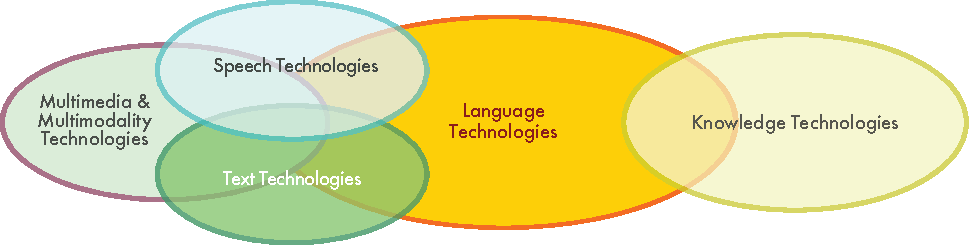
\includegraphics[width=\textwidth]{../_media/english/language_technologies}
  \caption{Language technology in context}
  \label{fig:ltincontext_en}
  \colorrule{grey3}{\textwidth}{1.5pt}
\end{figure*}

When we communicate, we combine language with other modes of communication and information media – for example speaking can involve gestures and facial expressions. Digital texts link to pictures and sounds. Movies may contain language in spoken and written form. In other words, speech and text technologies overlap and interact with other multimodal communication and multimedia technologies.\\ 
In this section, we will discuss the main application areas of language technology, i.\,e., language checking, web search, speech interaction, and machine translation. These applications and basic technologies include 

\begin{itemize}
\item spelling correction
\item authoring support
\item computer-assisted language learning
\item information retrieval 
\item information extraction
\item text summarisation
\item question answering
\item speech recognition 
\item speech synthesis 
\end{itemize}

\begin{figure*}[b]
  \colorrule{grey3}{\textwidth}{1.5pt}
  \center
  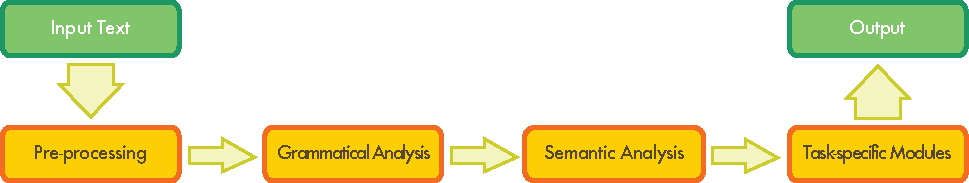
\includegraphics[width=\textwidth]{../_media/english/text_processing_app_architecture}
  \caption{A typical text processing architecture}
  \label{fig:textprocessingarch_en}
  \colorrule{grey3}{\textwidth}{1.5pt}
\end{figure*}

Language technology is an established area of research with an extensive set of introductory literature. The interested reader is referred to the following references:  \cite{carstensen-etal1, jurafsky-martin01, manning-schuetze1, lt-world1, lt-survey1}.

Before discussing the above application areas, we will briefly describe the architecture of a typical LT system.

\subsection{Application Architectures}

Software applications for language processing typically consist of several components that mirror different aspects of language. While such applications are typically very complex, figure~\ref{fig:textprocessingarch_en} shows a highly simplified architecture of a typical text processing system. The first three modules handle the structure and meaning of the text input:

\begin{enumerate}
\item Pre-processing: cleans the data, analyses or removes formatting, detects the input languages, and so on.
\item Grammatical analysis: finds the verb, its objects, modifiers and other parts of speech; detects the sentence structure.
\item Semantic analysis: performs disambiguation (i.\,e., computes the appropriate meaning of words in a given context); resolves anaphora (i.\,e., which pronouns refer to which nouns in the sentence); represents the meaning of the sentence in a machine-readable way.
\end{enumerate}

After analysing the text, task-specific modules can perform other operations, such as automatic summarisation and database look-ups.

In the remainder of this section, we firstly introduce the core application areas for language technology, and follow this with a brief overview of the state of LT research and education today, and a description of past and present research programmes. Finally, we present an expert estimate of core LT tools and resources for Bulgarian in terms of various dimensions such as availability, maturity and quality. The general situation of LT for the Bulgarian language is summarised in a matrix (figure~\ref{fig:lrlttable_en}). Tools and resources that are boldfaced in the text can also be found in figure~\ref{fig:lrlttable_en} (p.~\pageref{fig:lrlttable_en}) at the end of this chapter. LT support for Bulgarian is also compared to other languages that are part of this series.

\subsection{Core Application Areas}

In this section, we focus on the most important LT tools and resources, and provide an overview of LT activities in Bulgaria. 

\subsubsection{Language Checking}

\begin{figure*}[t]
  \colorrule{grey3}{\textwidth}{1.5pt}
  \center
  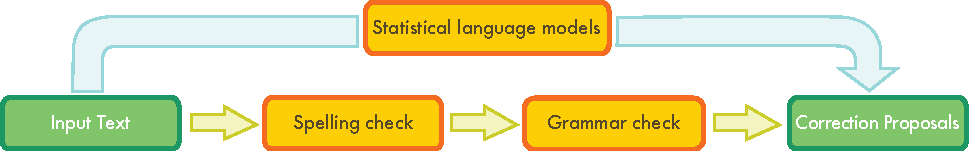
\includegraphics[width=\textwidth]{../_media/english/language_checking}
  \caption{Language checking (top: statistical; bottom: rule-based)}
  \label{fig:langcheckingaarch_en}
  \colorrule{grey3}{\textwidth}{1.5pt}
\end{figure*}

Anyone who has used a word processor such as Microsoft Word knows that it has a spell checker that highlights spelling mistakes and proposes corrections. The first spelling correction programs compared a list of extracted words against a dictionary of correctly spelled words. Today these programs are far more sophisticated. Using language-dependent algorithms for \textbf{grammatical analysis}, they detect errors related to morphology (e.\,g., plural formation) as well as syntax–related errors, such as a missing verb or a conflict of verb-subject agreement  (e.\,g., \textit{Tya *napisahme pismoto} [she *write a letter]). However, most spell checkers will not find any errors in the following text \cite{zar1}:

\begin{quote}
  I have a spelling checker,\\
  It came with my PC.\\
  It plane lee marks four my revue\\
  Miss steaks aye can knot sea.
\end{quote}

Handling these kinds of errors usually requires an analysis of the context, e.g., to decide if a word needs to be written in upper case, as in:

\begin{itemize}
\item Tya zhivee v \textbf{Stara} Zagora.
\item {[}She lives in Stara Zagora.{]} 
\item Tya e \textbf{stara} zhena.
\item {[}She is an old woman.{]}
\end{itemize}

This type of analysis either needs to draw on language-specific \textbf{grammars} laboriously coded into the software by experts, or on a statistical language model. In this case, a model calculates the probability of a particular word as it occurs in a specific position (e.g., between the words that precede and follow it). A statistical language model can be automatically created by using a large amount of (correct) language data (called a \textbf{text corpus}). These two approaches have been mostly developed around English language data. Neither approach can transfer easily to Bulgarian because the language has a flexible word orderand a richer inflection system. 

Language checking is not limited to word processors; it is also used in “authoring support systems”, i.\,e., software environments in which manuals and other types of technical documentation for complex IT, healthcare, engineering and other products, are written. To offset customer complaints about incorrect use and damage claims resulting from poorly understood instructions, companies are increasingly focusing on the quality of technical documentation while targeting the international market (via translation or localisation) at the same time. Advances in natural language processing have led to the development of authoring support software, which helps the writer of technical documentation to use vocabulary and sentence structures that are consistent with industry rules and (corporate) terminology restrictions.

\boxtext{Language checking is not limited to word processors but also applies to authoring systems.}

Besides spell checkers and authoring support, language checking is also important in the field of computer-assisted language learning. 
Language checking applications also automatically correct search engine queries, as found in Google's \textit{Did you mean \dots} suggestions.

\subsubsection{Web Search}

\begin{figure*}[htb]
  \colorrule{grey3}{\textwidth}{1.5pt}
  \center
  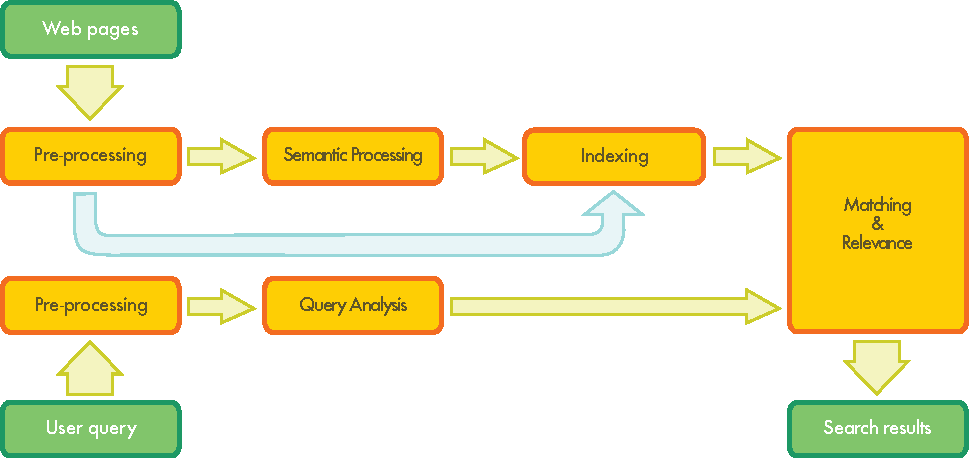
\includegraphics[width=\textwidth]{../_media/english/web_search_architecture}
  \caption{Web search}
  \label{fig:websearcharch_en}
  \colorrule{grey3}{\textwidth}{1.5pt}
 \end{figure*}

Searching the Web, intranets or digital libraries is probably the most widely used yet largely underdeveloped language technology application today. The Google search engine, which started in 1998, now handles about 80\% of all search queries \cite{spi1}. 
%Since 2004, the verb googeln even has an entry in the Duden dictionary. 
The Google search interface and results page display has not significantly changed since the first version. However, in the current version, Google offers spelling correction for misspelled words and incorporates basic semantic search capabilities that can improve search accuracy by analysing the meaning of terms in a search query context \cite{pc1}. The Google success story shows that a large volume of data and efficient indexing techniques can deliver satisfactory results using a statistical approach to language processing. 

For more sophisticated information requests, it is essential to integrate deeper linguistic knowledge to facilitate text interpretation. Experiments using \textbf{lexical resources} such as machine-readable thesauri or ontological language resources (e.\,g., WordNet for English or BulNet for Bulgarian) have demonstrated improvements in finding pages using synonyms of the original search terms, such as {\it atomna energiya} [atomic energy] and {\it yadrena energiya} [nuclear energy], or even more loosely related terms. 

\boxtext{The next generation of search engines\\ will have to include much more sophisticated language technology.}

The next generation of search engines will have to include much more sophisticated language technology, especially to deal with search queries consisting of a question or other sentence type rather than a list of keywords. For the query, \textit{Give me a list of all companies that were taken over by other companies in the last five years}, a syntactic as well as \textbf{semantic analysis} is required. The system also needs to provide an index to quickly retrieve relevant documents. A satisfactory answer will require syntactic parsing to analyse the grammatical structure of the sentence and determine that the user wants companies that have been acquired, rather than companies that have acquired other companies. For the expression \textit{last five years}, the system needs to determine the relevant range of years, taking into account the present year. The query then needs to be matched against a huge amount of unstructured data to find the pieces of information that are relevant to the user’s request. This process is called information retrieval, and involves searching and ranking relevant documents. To generate a list of companies, the system also needs to recognise a particular string of words in a document represents a company name, using a process called named entity recognition.

A more demanding challenge is matching a query in one language with documents in another language. Cross-lingual information retrieval involves automatically translating the query into all possible source languages and then translating the results back into the user's target language.

Now that data is increasingly found in non-textual formats, there is a need for services that deliver multimedia information retrieval by searching images, audio files and video data. In the case of audio and video files, a speech recognition module must convert the speech content into text (or into a phonetic representation) that can then be matched against a user query.

Certain Bulgarian portals have crawler software similar to those used by global search engines designed to index sites included within its categories. For example, Dir.bg, one of the first and largest web portals in Bulgaria launched a standalone service – Diri.bg. Diri (in Bulgarian {дири}) is an old word for ‘search’. 

Open source technologies like Lucene and Solr are often used by search-focused companies to provide a basic search infrastructure. Other search-based companies rely on international search technologies such as FAST (a Norwegian company acquired by Microsoft in 2008) or the French company Exalead (acquired by Dassault Systèmes in 2010). These companies focus their development on providing add-ons and advanced search engines for portals by using topic-relevant semantics. Due to the constant high demand for processing power, such search engines are only cost-effective when handling relatively small text corpora. The processing time is several thousand times higher than that needed by a standard statistical search engine like Google. These search engines are in high demand for topic-specific domain modelling, but they cannot be used on the Web with its billions and billions of documents.

\subsubsection{Speech Interaction}

Speech interaction is one of many application areas that depend on speech technology, i.\,e., technologies for processing spoken language. Speech interaction technology is used to create interfaces that enable users to interact in spoken language instead of using a graphical display, keyboard and mouse.  Today, these voice user interfaces (VUI) are used for partially or fully automated telephone services provided by companies to customers, employees or partners. Business domains that rely heavily on VUIs include banking, supply chain, public transportation, and telecommunications. Other uses of speech interaction technology include interfaces to car navigation systems and the use of spoken language as an alternative to the graphical or touchscreen interfaces in smartphones. Speech interaction technology comprises four technologies: 

\begin{figure*}[htb]
  \colorrule{grey3}{\textwidth}{1.5pt}
  \center
  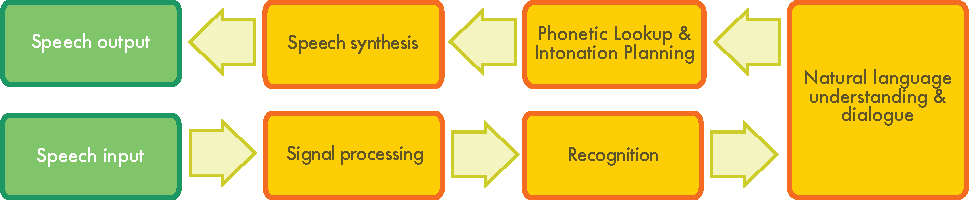
\includegraphics[width=\textwidth]{../_media/english/simple_speech-based_dialogue_architecture}
  \caption{Speech-based dialogue system}
  \label{fig:dialoguearch_en}
  \colorrule{grey3}{\textwidth}{1.5pt}
\end{figure*}

\begin{enumerate}
\item Automatic \textbf{speech recognition} (ASR) determines which words are actually spoken in a given sequence of sounds uttered by a user.  
\item Natural language understanding analyses the syntactic structure of a user’s utterance and interprets it according to the system in question.
\item Dialogue management determines which action to take given the user input and system functionality.   
\item \textbf{Speech synthesis} (text-to-speech or TTS) transforms the system’s reply into sounds for the user.
\end{enumerate}

One of the major challenges of ASR systems is to accurately recognise the words a user utters. This means restricting the range of possible user utterances to a limited set of keywords, or manually creating language models that cover a large range of natural language utterances. Using machine learning techniques, language models can also be generated automatically from \textbf{speech corpora}, i.\,e., large collections of speech audio files and text transcriptions. Restricting utterances usually forces people to use the voice user interface in a rigid way and can damage user acceptance; but the creation, tuning and maintenance of rich language models will significantly increase costs. VUIs that employ language models and initially allow a user to express their intent more flexibly -- prompted by a \textit{How may I help you?} greeting -- are better accepted by users.

\boxtext{Speech interaction is the basis for interfaces that allow a user to interact with spoken language.}

Companies tend to use pre-recorded utterances by professional speakers for generating the output of the voice user interface. For static utterances where the wording does not depend on particular contexts of use or personal user data, this can deliver a rich user experience. But more dynamic content in an utterance may suffer from unnatural intonation because bits of audio files have simply been strung together. Through optimisation, today’s TTS systems are getting better at producing natural-sounding dynamic utterances.

Interfaces in speech interaction have been considerably standardised during the last decade in terms of their various technological components. There has also been strong market consolidation in speech recognition and speech synthesis. The national markets in the G20 countries (economically resilient countries with high populations) have been dominated by just five global players, with Nuance (USA) and Loquendo (Italy) being the most prominent players in Europe. In 2011, Nuance announced the acquisition of Loquendo, which represents a further step in market consolidation.

On the Bulgarian TTS market, there are a few Bulgarian text-to-speech systems. One of these is SpeechLab 2.0 provided free-of-charge to computer users with visual disabilities. Only a few companies such as "Ciela" – a Bulgarian publisher of legal literature — have developed their own system for Bulgarian speech recognition. Finally, within the area of Speech Interaction, the is as yet no real market for syntactic and semantic analysis-based core technologies. 

The demand for voice user interfaces in Bulgaria has grown fast in the last five years, driven by increasing demand for customer self-service, cost optimisation for automated telephone services, and the increasing acceptance of spoken language as a media for human-machine interaction. 

Looking ahead, there will be significant changes, due to the spread of smartphones as a new platform for managing customer relationships, in addition to fixed telephones, the Internet and e-mail. This will also affect how speech interaction technology is used. In the long term, there will be fewer telephone-based VUIs, and spoken language apps will play a far more central role as a user-friendly input for smartphones. This will be largely driven by stepwise improvements in the accuracy of speaker-independent speech recognition via the speech dictation services already offered as centralised services to smartphone users.

\subsubsection{Machine Translation}

The idea of using digital computers to translate natural languages can be traced back to 1946 and was followed by substantial funding for research during the 1950s and again in the 1980s. Yet \textbf{machine translation} (MT) still cannot deliver on its initial promise of providing across-the-board automated translation.

\boxtext{At its basic level, Machine Translation simply substitutes words in one natural language with words in another language.}

The most basic approach to machine translation is the automatic replacement of the words in a text written in one natural language with the equivalent words of another language. This can be useful in subject domains that have a very restricted, formulaic language such as weather reports.  However, in order to produce a good translation of less restricted texts, larger text units (phrases, sentences, or even whole passages) need to be matched to their closest counterparts in the target language. The major difficulty is that human language is ambiguous. Ambiguity creates challenges on multiple levels, such as word sense disambiguation on the lexical level (a \textit{jaguar} is a brand of car or an animal) or the assignment of case on the syntactic level, for example:

\begin{itemize}
\item Politsayat nablyudava prestapnika s tele-skopa.
\item[] [The policeman observed the man with the telescope.]
\end{itemize}

\begin{itemize}
\item Politsayat nablyudava prestapnika s pistoleta.
\item[] [The policeman observed the man with the revolver.]
\end{itemize}

One way to build an MT system is to use linguistic rules. For translations between closely related languages, a translation using direct substitution may be feasible in cases such as the above example. However, rule-based (or linguistic knowledge-driven) systems often analyse the input text and create an intermediary symbolic representation from which the target language text can be generated. The success of these methods is highly dependent on the availability of extensive lexicons with morphological, syntactic, and semantic information, and large sets of grammar rules carefully designed by skilled linguists. This is a very long and therefore costly process.

\begin{figure*}[htb]
  \colorrule{grey3}{\textwidth}{1.5pt}
  \center
  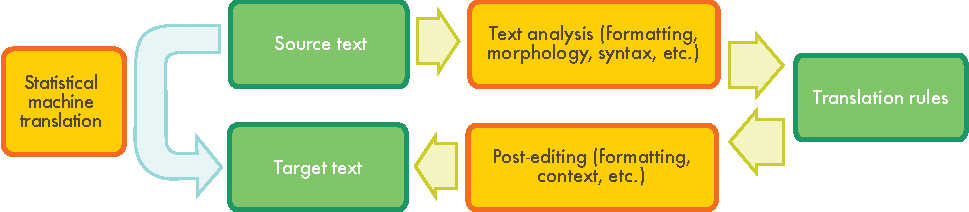
\includegraphics[width=\textwidth]{../_media/english/machine_translation}
  \caption{Machine translation (left: statistical; right: rule-based)}
  \label{fig:mtarch_en}
  \colorrule{grey3}{\textwidth}{1.5pt}
\end{figure*}
 
In the late 1980s when computational power increased and became cheaper, interest in statistical models for machine translation began to grow. Statistical models are derived from analysing bilingual text corpora, \textbf{parallel corpora}, such as the Europarl parallel corpus, which contains the proceedings of the European Parliament in 11 European languages. Given enough data, statistical MT works well enough to derive an approximate meaning of a foreign language text by processing parallel versions and finding plausible patterns of words. Unlike knowledge-driven systems, however, statistical (or data-driven) MT systems often generate ungrammatical output. Data-driven MT is advantageous because less human effort is required, and it can also cover special particularities of the language (e.\,g., idiomatic expressions) that are often ignored in knowledge-driven systems. 

\boxtext{Machine Translation is particularly\\ challenging for the Bulgarian language.}

The strengths and weaknesses of knowledge-driven and data-driven machine translation tend to be complementary, so that nowadays researchers focus on hybrid approaches that combine both methodologies. One such approach uses both knowledge-driven and data-driven systems, together with a selection module that decides on the best output for each sentence. However, results for sentences longer than, say, 12 words, will often be far from perfect. A more effective solution is to combine the best parts of each sentence from multiple outputs; this can be fairly complex, as corresponding parts of multiple alternatives are not always obvious and need to be aligned. 

For Bulgarian, MT is particularly challenging. The lack of noun case inflection; free word order and subject pro-drop pose problems for analysis. Extensive inflection in verb morphology is a challenge for generating words with proper markings. 

One of the good examples is WebTrance by SkyCode – a machine translation system which automatically translates texts, help files, menus, windows and internet pages from English, German, French, Spanish, Italian and Turkish into and from Bulgarian.  The use of machine translation can significantly increase productivity provided the system is intelligently adapted to user-specific terminology and integrated into a workflow. 

There is still a huge potential for improving the quality of MT systems. The challenges involve adapting language resources to a given subject domain or user area, and integrating the technology into workflows that already have term bases and translation memories. Another problem is that most of the current systems are English-centred and only support a few languages from and into Bulgarian. This leads to friction in the translation workflow and forces MT users to learn different lexicon coding tools for different systems.

Evaluation campaigns help to compare the quality of MT systems, their approaches and the status of the systems for different language pairs. Figure~\ref{fig:euromatrix_de} (p.~\pageref{fig:euromatrix_de}), which was prepared during the Euromatrix+ project, shows the pair-wise performances obtained for 22 of the 23 EU languages (Irish was not compared). The results are ranked according to a BLEU score, which indicates higher scores for better translations \cite{bleu1}. A human translator would normally achieve around 80 points. The best results (in green and blue) were achieved by languages that benefit from a considerable research effort in coordinated programmes and the existence of many parallel corpora (e.\,g., English, French, Dutch, Spanish and German). The languages with poorer results are shown in red. These either lack such development efforts or are structurally very different from other languages (e.\,g., Hungarian, Maltese, Finnish).

\subsection{Other Application Areas}

Building language technology applications involves a range of subtasks that do not always surface at the level of interaction with the user, but they provide significant service functionalities “behind the scenes” of the system in question. They all form important research issues that have now evolved into individual sub-disciplines of computational linguistics. Question answering, for example, is an active area of research for which annotated corpora have been built and scientific competitions have been initiated. The concept of question answering goes beyond keyword-based searches (in which the search engine responds by delivering a collection of potentially relevant documents) and enables users to ask a concrete question to which the system provides a single answer. For example:

\begin{itemize}
\item[] \textit{Question: How old was Neil Armstrong when he stepped on the moon?}
\item[] \textit{Answer: 38.}
\end{itemize}

While question answering is obviously related to the core area of web search, it is nowadays an umbrella term for such research issues as which different types of questions exist, and how they should be handled; how a set of documents that potentially contain the answer can be analysed and compared (do they provide conflicting answers?); and how specific information (the answer) can be reliably extracted from a document without ignoring the context. Question answering is in turn related to information extraction (IE), an area that was extremely popular and influential when computational linguistics took a statistical turn in the early 1990s. IE aims to identify specific pieces of information in specific classes of documents, such as the key players in company takeovers as reported in newspaper stories. Another common scenario that has been studied is reports on terrorist incidents. The task here consists of mapping appropriate parts of the text to a template that specifies the perpetrator, target, time, location and results of the incident. Domain-specific template-filling is the central characteristic of IE, which makes it another example of a “behind the scenes” technology that forms a well-demarcated research area, which in practice needs to be embedded into a suitable application environment.

\boxtext{Language technology applications often provide significant service functionalities behind the scenes of larger software systems.}

Text summarisation and \textbf{text generation} are two borderline areas that can act either as standalone applications or play a supporting role. Summarisation attempts to give the essentials of a long text in a short form, and is one of the features available in Microsoft Word. It mostly uses a statistical approach to identify the “important” words in a text (i.\,e., words that occur very frequently in the text in question but less frequently in general language use) and determine which sentences contain the most of these “important” words. These sentences are then extracted and put together to create the summary. In this very common commercial scenario, summarisation is simply a form of sentence extraction, and the text is reduced to a subset of its sentences. An alternative approach, for which some research has been carried out, is to generate brand new sentences that do not exist in the source text.

\boxtext{For Bulgarian, research in most text technologies is much less developed than for English.}

This requires a deeper understanding of the text, which means that so far this approach is far less robust. On the whole, a text generator is rarely used as a stand-alone application but is embedded into a larger software environment, such as a clinical information system that collects, stores and processes patient data. Creating reports is just one of many applications for text summarisation. 
For the Bulgarian language, research in these text technologies is much less developed than for the English language. Question answering, information extraction, and summarisation have been the focus of numerous open competitions in the USA since the 1990s, primarily organised by the government-sponsored organisations DARPA and NIST. These competitions have significantly improved the state of the art, but their focus has mostly been on the English language. As a result, there are hardly any annotated corpora or other special resources for these tasks in Bulgarian. When summarisation systems use purely statistical methods, they are largely language-independent and a number of research prototypes are available. For text generation, reusable components have traditionally been limited to surface realisation modules (generation grammars) and most of the available software is for the English language. 

\subsection{Educational Programmes}

Language technology is a very interdisciplinary field that involves the combined expertise of linguists, computer scientists, mathematicians, philosophers, psycholinguists, and neuroscientists among others. As a result, it has not acquired a clear, independent existence in the Bulgarian faculty system. In Bulgarian universities courses in computational linguistics are only partially available. They are usually designed either for humanities students or mathematicians but not both. Two years ago the University of Plovdiv began to offer a Bachelors programme in Linguistics with Information Technologies. 30 students enrolled in 2009-2010 and twice that number in 2010-2011. Students are offered a wide range of courses connected with the fundamentals of linguistics, mathematics and programming as well as language technology applications. The Bachelors degree in Informatics at the University of Plovdiv traditionally offers a lecture course in Computational Linguistics. 

Since 2004 the Faculty of Mathematics and Informatics of the University of Sofia has been offering a Masters programme in Artificial Intelligence. The University of Sofia also offers a Masters programme in Computational Linguistics. The programme includes subjects from the sphere of mathematics, logic, programming and theoretical linguistics. Graduates possess a good grounding to begin academic research in the area of computational linguistics as well as broader computational and linguistic literacy allowing them ability to develop unconventional practical applications. The success of the programme is evident from the professional development of the students from the previous intakes. They are employed in leading IT companies, popular national and specialised media and particularly in academic research.
The education of language technology in sufficient numbers is a prerequisite for the diverse research and thus the development of successful commercial activity.

\subsection[National Projects and Initiatives]{National Projects\newline and Initiatives}

The first international and national funding supporting language technologies for Bulgarian began at the very beginning of 1990s. Over a short period of time financing for a number of research projects from European institutions was got: LaTeSLav (Language Processing Technologies for Slavic Languages, 1991-1994) – aimed at developing a prototype of a grammar checker, BILEDITA (Bilingual Electronic Dictionaries and Intelligent Text Alignment, 1996-1998) – for the development of bi-lingual electronic dictionaries, GLOSSER (Support of Second Language Acquisition and Learning from Aligned Corpora, 1996-1998) – aimed at supporting foreign language training and others. The Multext-East (Multilingual Text Tools and Corpora for Central and Eastern European Languages, 1995-1997) extension of the previous Multext and EAGLES (European Commission's Expert Advisory Group on Language Engineering Standards) EU projects provided the Bulgarian language resources in a standardised format
  with standard mark-up and annotation, and these resources were later expanded and upgraded in the ELAN (European Language Activity Network, 1998-1999), TELRI I in II (Trans European Language Resources Infrastructure, 1995-1998 / 1999-2001) and Concede (Consortium for Central European Dictionary Encoding, 1998-2000) projects.

The Ministry of Education, Youth and Research through the National Scientific Fund (NSF), has supported research through national research programs. These programs have impelled numerous research projects and collaboration with international research centres and companies. The basis of technology development and commercial applications for automated processing of the Bulgarian language has been partly created as a result of these projects.

A number of years ago five Bulgarian academic institutions founded a consortium to create and develop an integrated national academic infrastructure for language resources. Bulgarian institutions are also involved in the CLARIN project (Common Language Resources and Technology Infrastructure). Other ongoing projects include those comprised by EUROPEANA aimed at developing the basic technologies and standards necessary to make knowledge on the Internet more widely available in the future. In addition to many other smaller-scale funded projects, the above-mentioned projects have led to the development of competences in the field of Language Technology as well as a basic technological infrastructure of language tools and resources for Bulgarian. However, public funding for LT projects in Bulgaria is dramatically lower than that for comparable projects in Europe, as well as in comparison to investments into areas such as language translation and multilingual information access by
  the USA \cite{sprachtech}.  
  
\subsection{Availability of Tools and Resources}

Figure~\ref{fig:lrlttable_en} provides a rating for language technology support for the Bulgarian language. This rating of existing tools and resources was generated by leading experts in the field who provided estimates based on a scale from 0 (very low) to 6 (very high) using seven criteria.

\begin{figure*}[htb]
\centering
%\begin{tabular}{>{\columncolor{orange1}}p{.33\linewidth}ccccccc} % ORIGINAL
\begin{tabular}{>{\columncolor{orange1}}p{.33\linewidth}@{\hspace*{6mm}}c@{\hspace*{6mm}}c@{\hspace*{6mm}}c@{\hspace*{6mm}}c@{\hspace*{6mm}}c@{\hspace*{6mm}}c@{\hspace*{6mm}}c}
\rowcolor{orange1}
 \cellcolor{white}&\begin{sideways}\makecell[l]{Quantity}\end{sideways}
&\begin{sideways}\makecell[l]{\makecell[l]{Availability} }\end{sideways} &\begin{sideways}\makecell[l]{Quality}\end{sideways}
&\begin{sideways}\makecell[l]{Coverage}\end{sideways} &\begin{sideways}\makecell[l]{Maturity}\end{sideways} &\begin{sideways}\makecell[l]{Sustainability}\end{sideways} &\begin{sideways}\makecell[l]{Adaptability}\end{sideways} \\ \addlinespace
\multicolumn{8}{>{\columncolor{orange2}}l}{Language Technology: Tools, Technologies and Applications} \\ \addlinespace
Speech Recognition	&	1.6 &	0.8 &	2.4 &	2.4 &	1.6 &	1.6 &	0.8 \\ \addlinespace
Speech Synthesis &	1.6 &	0.8 &	2.4 &	2.4 &	1.6 &	1.6 &	0.8\\ \addlinespace
Grammatical analysis &	2.4 &	2 &	3.6 &	3.6 &	2.8 &	2.4 &	2.8\\ \addlinespace
Semantic analysis &	0.8 &	0.8 &	1.3 &	1.1 &	0.8 &	1.1 &	1.3\\ \addlinespace
Text generation &	0.8 &	0.8 &	1.6 &	1.6 &	1.6 &	0.8 &	0.8\\ \addlinespace
Machine translation &	2.4 &	1.6 &	1.6 &	1.6 &	1.6 &	1.6 &	2.4\\ \addlinespace
\multicolumn{8}{>{\columncolor{orange2}}l}{Language Resources: Resources, Data and Knowledge Bases} \\ \addlinespace
Text corpora &	2.8 &	2.4 &	3.2 &	2.4 &	3.2 &	2.4 &	2.8\\ \addlinespace
Speech corpora &	0.8 &	0.8 &	2.4 &	1.6 &	2.4 &	2.4 &	2.5\\ \addlinespace
Parallel corpora &	2.4 &	0.8 &	3.2 &	1.6 &	1.6 &	1.6 &	2.4\\ \addlinespace
Lexical resources &	2.4 &	2.8 &	3.6 &	2.8 &	3.2 &	3.2 &	3.2\\ \addlinespace
Grammars &	1.6 &	1.6 &	2.4 &	2.4 &	2.4 &	2.4 &	1.6\\
\end{tabular}
\caption{State of language technology support for Bulgarian}
\label{fig:lrlttable_en}
\end{figure*}

The key results for Bulgarian language technology can be summed up as follows:

\begin{itemize}
\item The more linguistic and semantic knowledge a tool draws on, the more gaps there are in the technology (information retrieval versus text semantics). There is a need for far more effort to support deep linguistic processing.

\item Research has been successful in designing particularly high quality software, but many of the resources are not standardised and cannot be sustained effectively. A concerted program is required to standardise data and interchange formats.

\item While some reference corpora of high quality and quantity exist, i.e. Bulgarian national corpus, large syntactically and semantically corpora annotated by experts are not available.  Again, the situation gets worse as the need for more deep linguistic and semantic information grows.

\item There is a lack of parallel corpora for machine translation. Translation from Bulgarian to English works best because this language pair has the most data available. 

\item There is a huge gap in multimedia data.
\end{itemize}

\subsection{Cross-language comparison}

The current state of LT support varies considerably from one language community to another. In order to compare the situation between languages, this section will present an evaluation based on two sample application areas (machine translation and speech processing) and one underlying technology (text analysis), as well as basic resources needed for building LT applications. The languages were categorised using the following five-point scale: 

\begin{enumerate}
\item Excellent support
\item Good support
\item Moderate support
\item Fragmentary support
\item Weak or no support
\end{enumerate}

Language Technology support was measured according to the following criteria:

\textbf{Speech Processing:} Quality of existing speech recognition technologies, quality of existing speech synthesis technologies, coverage of domains, number and size of existing speech corpora, amount and variety of available speech-based applications.

\textbf{Machine Translation:} Quality of existing MT technologies, number of language pairs covered, coverage of linguistic phenomena and domains, quality and size of existing parallel corpora, amount and variety of available MT applications.

\textbf{Text Analysis:} Quality and coverage of existing text analysis technologies (morphology, syntax, semantics), coverage of linguistic phenomena and domains, amount and variety of available applications, quality and size of existing (annotated) text corpora, quality and coverage of existing lexical resources (e.\,g., WordNet) and grammars.

\textbf{Resources:} Quality and size of existing text corpora, speech corpora and parallel corpora, quality and coverage of existing lexical resources and grammars.

\subsection{Conclusions}

\emph{In this series of white papers, we have made an important effort by assessing the language technology support for 30 European languages, and by providing a high-level comparison across these languages. By identifying the gaps, needs and deficits, the European language technology community and its related stakeholders are now in a position to design a large scale research and development programme aimed at building a truly multilingual, technology-enabled communication across Europe.}

The results of this white paper series show that there is a dramatic difference in language technology support for the various European languages. While there are good quality software and resources available for some languages and application areas, others, usually smaller languages, have substantial gaps. Many languages lack basic technologies for text analysis and the essential resources. Others have basic tools and resources but the implementation of for example semantic methods is still far away. Therefore a large-scale effort is needed to attain the ambitious goal of providing high-quality language technology support for all European languages, for example through high quality machine translation. 

Over the past decade a number of important electronic language resources for Bulgarian (dictionaries, corpora, lexical data bases) as well as programmes for their processing (word sense disambiguation tool, spell checking, etc..) have been developed. However, the scope of the resources and the range of tools are still very limited when compared to the resources and tools for the English language, and they are simply not sufficient in quality and quantity to develop the kind of technologies required to support a truly multilingual knowledge society.

Nor can we simply transfer technologies already developed and optimised for the English language to handle Bulgarian. English-based systems for parsing (syntactic and grammatical analysis of sentence structure) typically perform far less well on German texts, due to the specific characteristics of the Bulgarian language such as free word order or sibject ommision.
The Bulgarian language technology industry dedicated to transforming research into products is currently fragmented and disorganised. A number of specialised small and middle SMEs that are not robust enough to address the internal and the global market with a sustained strategy are working in the field.

Our findings show that the only alternative is to make a substantial effort to create LT resources for Bulgarian, and use them to drive forward researc, innovation and development. The need for large amounts of data and the extreme complexity of language technology systems makes it vital to develop a new infrastructure and a more coherent research organization to spur greater sharing and cooperation.

Finally there is a lack of continuity in research and development funding. Short-term coordinated programmes tend to alternate with periods of sparse or zero funding. In addition, there is an overall lack of coordination with programmes in other EU countries and at the European Commission level.

In general, it can be stated that in the last two decades language technology for Bulgarian was never supported by a consistently devised national funding scheme. The process of development of HLT applications, tools and resources for Bulgarian has been, therefore, a mixture of international projects extending their scope from Western European languages to Middle and Eastern Europe, also with a view of the EU enlargement process, national research funding, and the enthusiasm of researchers involved in LT.

We can therefore conclude that there is a desperate need for a large, coordinated initiative focused on overcoming the differences in language technology readiness for European languages as a whole. 

Bulgaria’s participation in
META-NET will make it possible to develop, standardise and make
available several important LT resources and thus contribute to the
growth of Bulgarian language technology.

The long term goal of META-NET is to enable the creation of high-quality language technology for all languages. This requires all stakeholders - in politics, research, business, and society - to unite their efforts. The resulting technology will help tear down existing barriers and build bridges between Europe’s languages, paving the way for political and economic unity through cultural diversity. 
\end{multicols}

\clearpage

\begin{figure*}[t]
  \small
  \centering
  \begin{tabular}
  { % defines color for each column.
  >{\columncolor{corange5}}p{.13\linewidth}@{\hspace{.040\linewidth}}
  >{\columncolor{corange4}}p{.13\linewidth}@{\hspace{.040\linewidth}}
  >{\columncolor{corange3}}p{.13\linewidth}@{\hspace{.040\linewidth}}
  >{\columncolor{corange2}}p{.13\linewidth}@{\hspace{.040\linewidth}}
  >{\columncolor{corange1}}p{.13\linewidth} 
  }
  \multicolumn{1}{>{\columncolor{white}}c@{\hspace{.040\linewidth}}}{\textbf{Excellent}} & 
  \multicolumn{1}{@{}>{\columncolor{white}}c@{\hspace{.040\linewidth}}}{\textbf{Good}} &
  \multicolumn{1}{@{}>{\columncolor{white}}c@{\hspace{.040\linewidth}}}{\textbf{Moderate}} &
  \multicolumn{1}{@{}>{\columncolor{white}}c@{\hspace{.040\linewidth}}}{\textbf{Fragmentary}} &
  \multicolumn{1}{@{}>{\columncolor{white}}c}{\textbf{Weak/no}} \\ 
  \multicolumn{1}{>{\columncolor{white}}c@{\hspace{.040\linewidth}}}{\textbf{support}} & 
  \multicolumn{1}{@{}>{\columncolor{white}}c@{\hspace{.040\linewidth}}}{\textbf{support}} &
  \multicolumn{1}{@{}>{\columncolor{white}}c@{\hspace{.040\linewidth}}}{\textbf{support}} &
  \multicolumn{1}{@{}>{\columncolor{white}}c@{\hspace{.040\linewidth}}}{\textbf{support}} &
  \multicolumn{1}{@{}>{\columncolor{white}}c}{\textbf{support}} \\ \addlinespace
  
& \vspace*{0.5mm}English
& \vspace*{0.5mm}
Czech \newline 
Dutch \newline 
Finnish \newline 
French \newline 
German \newline   
Italian \newline  
Portuguese \newline 
Spanish \newline
& \vspace*{0.5mm}Basque \newline 
Bulgarian \newline 
Catalan \newline 
Danish \newline 
Estonian \newline 
Galician\newline 
Greek \newline  
Hungarian  \newline
Irish \newline  
Norwegian \newline 
Polish \newline 
Serbian \newline 
Slovak \newline 
Slovene \newline 
Swedish \newline
& \vspace*{0.5mm}
Croatian \newline 
Icelandic \newline  
Latvian \newline 
Lithuanian \newline 
Maltese \newline 
Romanian\\
\end{tabular}
\caption{Speech processing: state of language technology support for 30 European languages}
\label{fig:speech_cluster_en}
\end{figure*}

\begin{figure*}[b]
  \small
  \centering
  \begin{tabular}
  { % defines color for each column.
  >{\columncolor{corange5}}p{.13\linewidth}@{\hspace{.040\linewidth}}
  >{\columncolor{corange4}}p{.13\linewidth}@{\hspace{.040\linewidth}}
  >{\columncolor{corange3}}p{.13\linewidth}@{\hspace{.040\linewidth}}
  >{\columncolor{corange2}}p{.13\linewidth}@{\hspace{.040\linewidth}}
  >{\columncolor{corange1}}p{.13\linewidth} 
  }
  \multicolumn{1}{>{\columncolor{white}}c@{\hspace{.040\linewidth}}}{\textbf{Excellent}} & 
  \multicolumn{1}{@{}>{\columncolor{white}}c@{\hspace{.040\linewidth}}}{\textbf{Good}} &
  \multicolumn{1}{@{}>{\columncolor{white}}c@{\hspace{.040\linewidth}}}{\textbf{Moderate}} &
  \multicolumn{1}{@{}>{\columncolor{white}}c@{\hspace{.040\linewidth}}}{\textbf{Fragmentary}} &
  \multicolumn{1}{@{}>{\columncolor{white}}c}{\textbf{Weak/no}} \\ 
  \multicolumn{1}{>{\columncolor{white}}c@{\hspace{.040\linewidth}}}{\textbf{support}} & 
  \multicolumn{1}{@{}>{\columncolor{white}}c@{\hspace{.040\linewidth}}}{\textbf{support}} &
  \multicolumn{1}{@{}>{\columncolor{white}}c@{\hspace{.040\linewidth}}}{\textbf{support}} &
  \multicolumn{1}{@{}>{\columncolor{white}}c@{\hspace{.040\linewidth}}}{\textbf{support}} &
  \multicolumn{1}{@{}>{\columncolor{white}}c}{\textbf{support}} \\ \addlinespace
  
& \vspace*{0.5mm} English 
& \vspace*{0.5mm} 
French \newline 
Spanish
& \vspace*{0.5mm}
Catalan \newline 
Dutch \newline 
German \newline 
Hungarian \newline
Italian \newline 
Polish \newline 
Romanian \newline 
& \vspace*{0.5mm}Basque \newline 
Bulgarian \newline 
Croatian \newline 
Czech \newline
Danish \newline 
Estonian \newline 
Finnish \newline 
Galician \newline 
Greek \newline 
Icelandic \newline 
Irish \newline 
Latvian \newline 
Lithuanian \newline 
Maltese \newline 
Norwegian \newline 
Portuguese \newline 
Serbian \newline 
Slovak \newline 
Slovene \newline 
Swedish \newline 
\end{tabular}
\caption{Machine translation: state of language technology support for 30 European languages}
\label{fig:mt_cluster_en}
\end{figure*}

\begin{figure*}[t]
  \small
  \centering
  \begin{tabular}
  { % defines color for each column.
  >{\columncolor{corange5}}p{.13\linewidth}@{\hspace{.040\linewidth}}
  >{\columncolor{corange4}}p{.13\linewidth}@{\hspace{.040\linewidth}}
  >{\columncolor{corange3}}p{.13\linewidth}@{\hspace{.040\linewidth}}
  >{\columncolor{corange2}}p{.13\linewidth}@{\hspace{.040\linewidth}}
  >{\columncolor{corange1}}p{.13\linewidth} 
  }
  \multicolumn{1}{>{\columncolor{white}}c@{\hspace{.040\linewidth}}}{\textbf{Excellent}} & 
  \multicolumn{1}{@{}>{\columncolor{white}}c@{\hspace{.040\linewidth}}}{\textbf{Good}} &
  \multicolumn{1}{@{}>{\columncolor{white}}c@{\hspace{.040\linewidth}}}{\textbf{Moderate}} &
  \multicolumn{1}{@{}>{\columncolor{white}}c@{\hspace{.040\linewidth}}}{\textbf{Fragmentary}} &
  \multicolumn{1}{@{}>{\columncolor{white}}c}{\textbf{Weak/no}} \\ 
  \multicolumn{1}{>{\columncolor{white}}c@{\hspace{.040\linewidth}}}{\textbf{support}} & 
  \multicolumn{1}{@{}>{\columncolor{white}}c@{\hspace{.040\linewidth}}}{\textbf{support}} &
  \multicolumn{1}{@{}>{\columncolor{white}}c@{\hspace{.040\linewidth}}}{\textbf{support}} &
  \multicolumn{1}{@{}>{\columncolor{white}}c@{\hspace{.040\linewidth}}}{\textbf{support}} &
  \multicolumn{1}{@{}>{\columncolor{white}}c}{\textbf{support}} \\ \addlinespace

& \vspace*{0.5mm}English
& \vspace*{0.5mm}
  Dutch \newline 
  French \newline 
  German \newline 
  Italian \newline 
  Spanish
& \vspace*{0.5mm}Basque \newline 
  Bulgarian \newline 
  Catalan \newline 
  Czech \newline 
  Danish \newline 
  Finnish \newline 
  Galician \newline 
  Greek \newline 
  Hungarian \newline 
  Norwegian \newline 
  Polish \newline 
  Portuguese \newline 
  Romanian \newline 
  Slovak \newline 
  Slovene \newline 
  Swedish \newline 
& \vspace*{0.5mm}
  Croatian \newline 
  Estonian \newline 
  Icelandic \newline 
  Irish \newline 
  Latvian \newline 
  Lithuanian \newline 
  Maltese \newline 
  Serbian \\
  \end{tabular}
\caption{Text analysis: state of language technology support for 30 European languages}
\label{fig:text_cluster_en}
\end{figure*}

\begin{figure*}[b]
  \small
  \centering
  \begin{tabular}
  { % defines color for each column.
  >{\columncolor{corange5}}p{.13\linewidth}@{\hspace{.040\linewidth}}
  >{\columncolor{corange4}}p{.13\linewidth}@{\hspace{.040\linewidth}}
  >{\columncolor{corange3}}p{.13\linewidth}@{\hspace{.040\linewidth}}
  >{\columncolor{corange2}}p{.13\linewidth}@{\hspace{.040\linewidth}}
  >{\columncolor{corange1}}p{.13\linewidth} 
  }
  \multicolumn{1}{>{\columncolor{white}}c@{\hspace{.040\linewidth}}}{\textbf{Excellent}} & 
  \multicolumn{1}{@{}>{\columncolor{white}}c@{\hspace{.040\linewidth}}}{\textbf{Good}} &
  \multicolumn{1}{@{}>{\columncolor{white}}c@{\hspace{.040\linewidth}}}{\textbf{Moderate}} &
  \multicolumn{1}{@{}>{\columncolor{white}}c@{\hspace{.040\linewidth}}}{\textbf{Fragmentary}} &
  \multicolumn{1}{@{}>{\columncolor{white}}c}{\textbf{Weak/no}} \\ 
  \multicolumn{1}{>{\columncolor{white}}c@{\hspace{.040\linewidth}}}{\textbf{support}} & 
  \multicolumn{1}{@{}>{\columncolor{white}}c@{\hspace{.040\linewidth}}}{\textbf{support}} &
  \multicolumn{1}{@{}>{\columncolor{white}}c@{\hspace{.040\linewidth}}}{\textbf{support}} &
  \multicolumn{1}{@{}>{\columncolor{white}}c@{\hspace{.040\linewidth}}}{\textbf{support}} &
  \multicolumn{1}{@{}>{\columncolor{white}}c}{\textbf{support}} \\ \addlinespace
    
& \vspace*{0.5mm}English
& \vspace*{0.5mm} 
    Czech \newline 
    Dutch \newline 
    French \newline 
    German \newline 
    Hungarian \newline
    Italian \newline
    Polish \newline
    Spanish \newline
    Swedish \newline 
& \vspace*{0.5mm} Basque\newline 
    Bulgarian\newline 
    Catalan \newline 
    Croatian \newline 
    Danish \newline 
    Estonian \newline 
    Finnish \newline 
    Galician \newline 
    Greek \newline 
    Norwegian \newline 
    Portuguese \newline 
    Romanian \newline 
    Serbian \newline 
    Slovak \newline 
    Slovene \newline
&  \vspace*{0.5mm}
    Icelandic \newline 
    Irish \newline 
    Latvian \newline 
    Lithuanian \newline 
    Maltese  \\
  \end{tabular}
  \caption{Speech and text resources: State of support for 30 European languages}  
  \label{fig:resources_cluster_en}
\end{figure*}

\clearpage

% --------------------------------------------------------------------------
\ssection[About META-NET]{About META-NET}

\begin{multicols}{2}
META-NET is a Network of Excellence funded by the European Commission. The network currently consists of 54 members from 33 European countries \cite{rehm2011}. META-NET fosters the Multilingual Europe Technology Alliance (META), a growing community of language technology professionals and organisations in Europe. META-NET cooperates with other initiatives like the Common Language Resources and Technology Infrastructure (CLARIN), which is helping establish digital humanities research in Europe. META-NET fosters the technological foundations for a truly multilingual European information society that:

\begin{itemize}
\item makes communication and cooperation possible across languages;
\item provides equal access to information and knowledge in any language;
\item offers advanced and affordable networked information technology to European citizens.
\end{itemize}

META-NET stimulates and promotes multilingual technologies for all European languages. The technologies enable automatic translation, content production, information processing and knowledge management for a wide variety of applications and subject domains. The network wants to improve current approaches, so better communication and cooperation across languages can take place. Europeans have an equal right to information and knowledge regardless of language.

META-NET launched on 1 February 2010 with the goal of advancing research in language technology (LT). The network supports a Europe that unites as a single digital market and information space. META-NET has conducted several activities that further its goals. META-VISION, META-SHARE and META-RESEARCH are the network’s three lines of action.

\textbf{META-VISION} fosters a dynamic and influential stakeholder community that unites around a shared vision and a common strategic research agenda (SRA). The main focus of this activity is to build a coherent and cohesive LT community in Europe by bringing together representatives from highly fragmented and diverse groups of stakeholders. In the first year of META-NET, presentations at the FLaReNet Forum (Spain), Language Technology Days (Luxembourg), JIAMCATT 2010 (Luxembourg), LREC 2010 (Malta), EAMT 2010 (France) and ICT 2010 (Belgium) centred on public outreach. According to initial estimates, META-NET has already contacted more than 2,500 LT professionals to develop its goals and visions with them. At the META-FORUM 2010 event in Brussels, META-NET communicated the initial results of its vision building process to more than 250 participants. In a series of interactive sessions, the participants provided feedback on the visions presented by the network. 

\textbf{META-SHARE} creates an open, distributed facility for exchanging and sharing resources. The peer-to-peer network of repositories will contain language data, tools and web services that are documented with high-quality metadata and organised in standardised categories. The resources can be readily accessed and uniformly searched. The available resources include free, open source materials as well as restricted, commercially available, fee-based items. META-SHARE targets existing language data, tools and systems as well as new and emerging products that are required for building and evaluating new technologies, products and services. The reuse, combination, repurposing and re-engineering of language data and tools plays a crucial role. META-SHARE will eventually become a critical part of the LT marketplace for developers, localisation experts, researchers, translators and language professionals from small, mid-sized and large enterprises. META-SHARE addresses the full development cycle of LT—from research to innovative products and services. A key aspect of this activity is establishing META-SHARE as an important and valuable part of a European and global infrastructure for the LT community. 

\textbf{META-RESEARCH} builds bridges to related technology fields. This activity seeks to leverage advances in other fields and to capitalise on innovative research that can benefit language technology. In particular, this activity wants to bring more semantics into machine translation (MT), optimise the division of labour in hybrid MT, exploit context when computing automatic translations and prepare an empirical base for MT. META-RESEARCH is working with other fields and disciplines, such as machine learning and the Semantic Web community. META-RESEARCH focuses on collecting data, preparing data sets and organising language resources for evaluation purposes; compiling inventories of tools and methods; and organising workshops and training events for members of the community. This activity has already clearly identified aspects of MT where semantics can impact current best practices. In addition, the activity has created recommendations on how to approach the problem of integrating semantic information in MT. META-RESEARCH is also finalising a new language resource for MT, the Annotated Hybrid Sample MT Corpus, which provides data for English-German, English-Spanish and English-Czech language pairs. META-RESEARCH has also developed software that collects multilingual corpora that are hidden on the Web.
\end{multicols}

\vfill
\centerline{office@meta-net.eu -- http://www.meta-net.eu}

\cleardoublepage

\appendix
\addtocontents{toc}{\protect\bigskip}

\bsection[Цитирани източници -- References]{Цитирани източници --- References}
\bibliographystyle{unsrt} % What is the difference between "unsrt" und "is-unsrt"?
%\bibliographystyle{is-unsrt}
\bibliography{bulgarian_references}
  
\cleardoublepage

\bsection[Организации членки на META-NET -- META-NET
Members]{Организации членки на META-NET --- META-NET\ \ \ \ \ \ \ \ \ Members}
\label{metanetmembers}

\small

\begin{longtable}{@{}llp{110mm}@{}}
  Австрия & \textcolor{grey1}{Austria} & Zentrum für
  Translationswissenschaft, Universität Wien: Gerhard Budin\\
  \addlinespace 
  Белгия & \textcolor{grey1}{Belgium} & Computational Linguistics and
  Psycholinguistics Research Centre, University of Antwerp: Walter
  Daelemans\\ \addlinespace
  & & Centre for Processing Speech and Images, University of Leuven:\newline
Dirk van Compernolle \\ \addlinespace
  България & \textcolor{grey1}{Bulgaria} & Institute for Bulgarian
  Language, Bulgarian Academy of Sciences: Svetla Koeva \\
  \addlinespace
  Великобритания & \textcolor{grey1}{UK} & School of Computer Science, University of Manchester: Sophia Ananiadou \\ \addlinespace 
  & & Institute for Language, Cognition and Computation, Center for Speech Technology Research, University of Edinburgh: Steve Renals \\ \addlinespace 
  & & Research Institute of Informatics and Language Processing, University of Wolverhampton: Ruslan Mitkov \\ \addlinespace 
  Германия & \textcolor{grey1}{Germany} & Language Technology Lab, DFKI: Hans Uszkoreit, Georg Rehm\\ \addlinespace
  & & Human Language Technology and Pattern Recognition, RWTH Aachen University: Hermann Ney \\ \addlinespace
  & & Department of Computational Linguistics, Saarland University:
  Manfred Pinkal\\ \addlinespace 
  Гърция & \textcolor{grey1}{Greece} & R.C. “Athena”, Institute for Language and Speech Processing: Stelios Piperidis\\ \addlinespace
Дания &  \textcolor{grey1}{Denmark} & Centre for Language Technology,
University of Copenhagen: \newline Bolette Sandford Pedersen, Bente
Maegaard\\ \addlinespace
  Естония & \textcolor{grey1}{Estonia} & Institute of Computer
  Science, University of Tartu: Tiit Roosmaa, Kadri Vider\\
  \addlinespace
  Ирландия & \textcolor{grey1}{Ireland} & School of Computing, Dublin City University: Josef van Genabith\\ \addlinespace
  Исландия & \textcolor{grey1}{Iceland} & School of Humanities, University of Iceland: Eiríkur Rögnvaldsson\\ \addlinespace
  Испания & \textcolor{grey1}{Spain} & Barcelona Media: Toni Badia, Maite Melero \\ \addlinespace 
  & & Institut Universitari de Lingüística Aplicada, Universitat Pompeu Fabra: Núria Bel \\ \addlinespace 
  & & Aholab Signal Processing Laboratory, University of the Basque Country:\newline Inma Hernaez Rioja \\ \addlinespace 
  & & Center for Language and Speech Technologies and Applications, Universitat Politècnica de Catalunya:  Asunción Moreno \\ \addlinespace 
  & & Department of Signal Processing and Communications, University of Vigo:\newline Carmen García Mateo \\ \addlinespace 
  Италия & \textcolor{grey1}{Italy} & Consiglio Nazionale delle Ricerche, Istituto di Linguistica Computazionale “Antonio Zampolli”: Nicoletta Calzolari\\ \addlinespace
  & & Human Language Technology Research Unit, Fondazione Bruno Kessler:\newline Bernardo Magnini\\ \addlinespace 
  Кипър & \textcolor{grey1}{Cyprus} & Language Centre, School of
  Humanities: Jack Burston\\ \addlinespace
  Латвия & \textcolor{grey1}{Latvia} & Tilde: Andrejs Vasiļjevs\\ \addlinespace 
  & & Institute of Mathematics and Computer Science, University of
  Latvia: \newline Inguna Skadiņa\\ \addlinespace
  Литва & \textcolor{grey1}{Lithuania} & Institute of the Lithuanian Language: Jolanta Zabarskaitė\\ \addlinespace
  Люксембург & \textcolor{grey1}{Luxembourg} & Arax Ltd.: Vartkes Goetcherian\\ \addlinespace
  Малта & \textcolor{grey1}{Malta} & Department Intelligent Computer Systems, University of Malta: Mike Rosner\\ \addlinespace
  Норвегия & \textcolor{grey1}{Norway} & Department of Linguistic, University of Bergen: Koenraad De Smedt\\ \addlinespace 
  & & Department of Informatics, Language Technology Group, University of Oslo:\newline Stephan Oepen \\ \addlinespace
  Полша & \textcolor{grey1}{Poland} & Institute of Computer Science, Polish Academy of Sciences: Adam Przepiórkowski, Maciej Ogrodniczuk \\ \addlinespace
  & & University of Łódź: Barbara Lewandowska-Tomaszczyk, Piotr Pęzik\\ \addlinespace
  & & Department of Computer Linguistics and Artificial Intelligence, Adam Mickiewicz University: Zygmunt Vetulani \\ \addlinespace
  Португалия & \textcolor{grey1}{Portugal} & University of Lisbon: António Branco, Amália Mendes \\ \addlinespace
  & & Spoken Language Systems Laboratory, Institute for Systems Engineering and Computers: Isabel Trancoso \\ \addlinespace
  Румъния & \textcolor{grey1}{Romania} & Research Institute for Artificial Intelligence, Romanian Academy of Sciences:\newline Dan Tufiș \\ \addlinespace
  & & Faculty of Computer Science, University Alexandru Ioan Cuza of
  Iași: Dan Cristea \\ \addlinespace
  Словакия & \textcolor{grey1}{Slovakia} & Ľudovít Štúr Institute of Linguistics, Slovak Academy of Sciences: Radovan Garabík \\ \addlinespace 
  Словения & \textcolor{grey1}{Slovenia} & Jožef Stefan Institute: Marko Grobelnik \\ \addlinespace 
  Сърбия & \textcolor{grey1}{Serbia} & University of Belgrade, Faculty of Mathematics: Duško Vitas, Cvetana Krstev,\newline Ivan Obradović \\ \addlinespace
  & & Pupin Institute: Sanja Vranes \\ \addlinespace  
  Унгария & \textcolor{grey1}{Hungary} & Research Institute for Linguistics, Hungarian Academy of Sciences: Tamás Váradi\\  \addlinespace
  & & Department of Telecommunications and Media Informatics, Budapest University of Technology and Economics: Géza Németh, Gábor Olaszy\\ \addlinespace
  Финландия & \textcolor{grey1}{Finland} & Computational Cognitive
  Systems Research Group, Aalto University: \newline Timo Honkela\\ \addlinespace
  & & Department of Modern Languages, University of Helsinki: Kimmo
  Koskenniemi,\newline Krister Lindén \\ \addlinespace
  Франция & \textcolor{grey1}{France} & Centre National de la Recherche Scientifique, Laboratoire d'Informatique pour la Mécanique et les Sciences de l'Ingénieur and Institute for Multilingual and Multimedia Information: Joseph Mariani \\ \addlinespace
  & & Evaluations and Language Resources Distribution Agency: Khalid Choukri\\ \addlinespace 
  Холандия & \textcolor{grey1}{Netherlands} & Utrecht Institute of Linguistics, Utrecht University: Jan Odijk\\ \addlinespace 
  & & Computational Linguistics, University of Groningen: Gertjan van
  Noord\\ \addlinespace
  Хърватия & \textcolor{grey1}{Croatia} & Institute of Linguistics,
  Faculty of Humanities and Social Science, University of Zagreb:
  Marko Tadić \\ \addlinespace
  Чехия & \textcolor{grey1}{Czech Republic} & Institute of Formal and Applied Linguistics, Charles University in Prague: Jan Hajič \\ \addlinespace
  Швейцария & \textcolor{grey1}{Switzerland} & Idiap Research
  Institute: Hervé Bourlard \\ \addlinespace 
  Швеция & \textcolor{grey1}{Sweden} & Department of Swedish, University of Gothenburg: Lars Borin \\ \addlinespace 
\end{longtable}
\normalsize

\renewcommand*{\figureformat}{}
\renewcommand*{\captionformat}{}

\begin{figure*}[htbp]
  \colorrule{grey3}{\textwidth}{1.5pt}
  \center
  %\fbox{-- META-NET group picture omitted to keep the size of the PDF file small. --}
  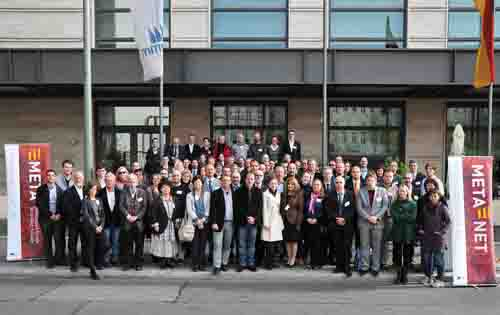
\includegraphics[width=\textwidth]{../_media/meta-net_team.jpg}
  \caption{Повече от 100 експерти в областта на езиковите технологии, представители на различни страни и езици в META-NET, обсъдиха и приеха онсовните резултати и послания на Серията Бели книги на срещата на  META-NET в Берлин, 21/22 октомври 2011. --- \textcolor{grey1}{About 100 language technology experts -- representatives of the countries and languages represented in META-NET -- discussed and finalised the key results and messages of the White Paper Series at a META-NET meeting in Berlin, Germany, on October 21/22, 2011.}}
  \medskip
  \colorrule{grey3}{\textwidth}{1.5pt}
\end{figure*}

\cleardoublepage

\bsection[Серия „Бели книги“ на META-NET -- The META-NET White Paper
Series]{Серия „Бели\ \ \ \ книги“ на META-NET --- The META-NET\ \ \ \ \ \ White Paper Series}
\label{whitepaperseries}

\vspace*{-5mm}
\centering
  \setlength{\tabcolsep}{2em}
  \begin{tabularx}{\textwidth}{lllll} \toprule\addlinespace
  &английски & English & English\\
  &баски & Basque & euskara\\
  &български & Bulgarian & български\\
  &галски & Galician & galego\\
  &гръцки & Greek & ελληνικά\\
  &датски & Danish & dansk\\
  &естонски & Estonian & eesti\\
  &ирландски & Irish & Gaeilge\\
  &исландски & Icelandic & íslenska\\
  &испански & Spanish & español\\
  &италиански & Italian & italiano\\
  &каталонски & Catalan & català\\
  &латвийски & Latvian & latviešu valoda\\
  &литовски & Lithuanian & lietuvių kalba\\
  &малтийски & Maltese & Malti\\
  &немски & German & Deutsch\\
  &норвежки Bokmål & Norwegian Bokmål & bokmål\\
  &норвежки Nynorsk & Norwegian Nynorsk & nynorsk\\
  &полски & Polish & polski\\
  &португалски & Portuguese & português\\
  &румънски & Romanian & română\\
  &словашки & Slovak & slovenčina\\
  &словенски & Slovene & slovenščina\\
  &сръбски & Serbian & српски\\
  &унгарски & Hungarian & magyar\\ 
  &фински & Finnish & suomi\\
  &френски & French & français\\
  &холандски & Dutch & Nederlands\\
  &хърватски & Croatian & hrvatski\\
  &чешки & Czech & čeština\\
  &шведски & Swedish & svenska\\ \addlinespace \bottomrule
\end{tabularx}

\end{document}
